% Delete the MSc option if you are doing a PhD, or replace it with MPhil
% for a Master of Philosophy thesis
%
% The 12pt option is required by the 2001/02 thesis regulations
% Last update 15th August 2007: new Abstract format and Copyright Statement

% Replace MSc with PhD for PhD theses
% Remove the twoside option for single-sided printing
\documentclass[12pt,oneside,PhD]{muthesis}

% Use this command to output a single chapter
%\includeonly{chapter_events}
%\includeonly{chapter_floodinundation}
%\includeonly{chapter_metdatamodels}
%\includeonly{conclusions}
\includeonly{chapter_LEMs}



\usepackage{rotating}
\usepackage[labelfont=bf]{caption}
\usepackage{lineno}
%\linenumbers
\usepackage{listings}
%\usepackage{epigraph}
\usepackage[dvipsnames]{xcolor}
\usepackage{textcomp}
\usepackage{hyperref}
\hypersetup{colorlinks=true,allcolors={blue!50!black}}
\usepackage{hypcap}
\usepackage{gensymb}  % degree symbol
\usepackage{subcaption}

%\usepackage[]{hyperref}
%\hypersetup{
%    pdftitle={PhD Thesis},
%    pdfauthor={Declan Valters},
%    pdf subject={Environmental Modelling},
%    pdfkeywords={Flooding, Erosion},
%    bookmarksnumbered=true,     
%    bookmarksopen=true,         
%    bookmarksopenlevel=1,       
%    colorlinks=true,            
%    pdfstartview=Fit,           
%    pdfpagemode=UseOutlines,    % this is the option you were lookin for
%    pdfpagelayout=TwoPageRight
%}

% IF USING BIBLATEX PACKAGE, BIBLIOGRAPHY FILE MUST
% GO HERE IN PREAMBLE
\bibliography{literature}

\makeatletter
\renewcommand{\@chapapp}{}% Not necessary...
\newenvironment{chapquote}[2][2em]
  {\setlength{\@tempdima}{#1}%
   \def\chapquote@author{#2}%
   \parshape 1 \@tempdima \dimexpr\textwidth-2\@tempdima\relax%
   \itshape}
  {\par\normalfont\hfill--\ \chapquote@author\hspace*{\@tempdima}\par\bigskip}
\makeatother


%these are now in the muthesis.cls file
%\usepackage[utf8]{inputenc}
%\usepackage{graphicx}
%\usepackage{amsmath}
%\usepackage{amsmath}
%\usepackage{amsfonts}
%\usepackage{amssymb}

\begin{document}

% This section contains the title, abstract, and all the things like table of
% contents, list of figures and tables etc.
\title{Linking numerical landscape evolution models with high-resolution meteorological data}

\author{Declan Valters}
% Faculty of Life Sciences people should comment the next line out
\school{Earth and Environmental Sciences}
\faculty{Science and Engineering}
\def\wordcount{74031}

% Uncomment the line below to suppress the `List of Tables' page (optional)
%\tablespagefalse

% Uncomment the line below to suppress the `List of Figures' page (optional)
%\figurespagefalse

% Uncomment the line below to use a customised Declaration statement
%\def\declaration{All the work in this thesis has been sourced from Google.}

\beforeabstract
The contribution of this thesis is twofold: 1) The development of a hydrodynamic landscape evolution model for use on high-performance computing systems and 2) Assessing the sensitivity of hydro-geomorphic processes to high-resolution rainfall input data using the model.

The thesis addresses a limitation in numerical landscape evolution models regarding how spatial variation in rainfall is represented or parameterised within such models. Typically, landscape evolution models forsake a realistic representation of rainfall patterns in favour of a simpler treatments of rainfall as being spatially homogeneous across the model domain. The simplification in rainfall inputs is still made despite the fact that many geomorphological processes are sensitive to thresholds of sediment entrainment and transport, driven by the distribution and movement of water within the landscape. 

The thesis starts by exploring current limitations in rainfall representation in landscape evolution models, and assesses various precipitation data sources that could be potentially used as more realistic rainfall inputs to landscape evolution models. A numerical model of landscape evolution is developed for deployment on high-performance parallel computing systems, based on the established CAESAR-Lisflood model \citep{Coulthard2013}. The new model code is benchmarked, showing performance benefits compared with the serial code. The improved model code is shown to produce results commensurate with the CAESAR-Lisflood model it is based on.

The model is applied to assessing the sensitivity of flood-inundation predictions, sediment flux, and erosion distribution within river catchments to spatial variation in rainfall during extreme storm events. Two real storm events that caused localised flash flooding in the UK are used a test cases: the Boscastle storm of 2004 and the North York Moors storm of 2005. 

Flood extent predictions and river discharges are found to be sensitive to the use of spatially variable input rainfall data, with high-resolution rainfall data leading to larger peak flood discharges. The role of sediment erosion during large floods is also assessed, but it is found to play a minor role relative to spatially variable rainfall data. In contrast, the geomorphological response of catchments (sediment flux and fluvial erosion) to single storm events is shown to be less sensitive to the spatial heterogeneity of rainfall input and controlled more strongly by the choice of erosional process parameterisation within the model.

%Finally, a software framework is presented for driving a landscape evolution model with input from a numerical weather prediction model. Using high-resolution NWP simulations of 250m grid spacing, mesoscale rainfall features are resolved at the river catchment scale. The UK storm case studies described in the previous chapter are re-assessed using data from NWP simulations of each case to investigate the response of catchments to the mesoscale details of severe rainfall events.
%To explore the effects of rainfall spatial variability at longer timescales of topographic evolution, the CHILD landscape evolution model (Tucker et al., 2001) is developed to incorporate a model of spatially-limited storm morphology. The rainfall model is designed to represent the typical intense rainfall associated with convective storm cells.


%
%
%From a meteorological perspective, precipitation patterns are observably non-uniform at a variety of scales, due to effects such as the orographic enhancement of rainfall, as well as the spatially limited nature of convective storm cells that bring intense rainfall. In temperate regions, many geomorphic processes are ultimately driven by the movement of water in the landscape, such as fluvial incision and sediment transport.
%
%Write your abstract here: Remember, it must fit on this A4 page and should
%describe contents of the thesis/dissertation. Here might also be a good place
%to indicate what you have achieved in the thesis/dissertation and, in the
%case of a PhD, what new results you have discovered. Note that for a PhD
%single-spacing is used throughout the Abstract, including displayed equations
%\[
%e = mc^{2}
%\]
%as for the above example.

\afterabstract
%
%% The next part is optional; however it is a good place to thank your
%% supervisor and the people responsible for providing computer support ;-)
%\prefacesection{Layperson's abstract}
%An optional section suggested by the UoM thesis preparation guide.
%
\prefacesection{Acknowledgements}
%%Writing this thesis has been an exercise in sustained suffering. The casual reader may, perhaps, exempt themselves from excessive guilt, but for those of you who have played the larger role in prolonging my agonies with your encouragement and support, well…you know who you are, and I hope you get what you deserve.
%
%I wish I could write that this PhD had been an enjoyable experience, but truth be told, on the whole it has been the most depressing, demoralising, and soul-destroying experience of my life. I would have quit several years ago, but carried on obstinately out of a vague notion of duty to those who have supported and encouraged me along the way. In all honesty, I regret doing this PhD and the years I have lost from undertaking it.
%\\ \\
\noindent
This work was funded by the Natural Environment Research Council doctoral training grant number NE/L501591/1.
\\~\\
\noindent
Data was provided by the British Atmospheric Data Centre, the Environment Agency (England), Ordnance Survey Open Data, and the UK National River Flow Archives. 
\\~\\
\noindent
This work used the ARCHER UK National Supercomputing Service (\url{http://www.archer.ac.uk}) and the Centre for Environmental Data Analysis JASMIN computing facility (\url{http://www.jasmin.ac.uk/}).
% The next line is NOT optional and MUST appear
\afterpreface



% Finally, you can start writing about all the new theorems you have proved
% and all the new results that you have discovered

%=-=-=-=-=-=-=-=-=-=-=-=
% MOTIVATION, BACKGROUND
%=-=-=-=-=-=-=-=-=-=-=-=

% Chapter 1 is a concise overview of the scientfic and technological background to the work.
\chapter{Introduction}
\label{chapter_intro}
%
%\begin{chapquote}{Leonardo da Vinci \textit{}}
%``Water is the driving force of all nature...''
%\end{chapquote}

\section{Overview}

Intense rainfall has the power to cause flash flooding and drive rapid landscape change in a single storm. Rainfall input to river catchments is one of several controls on runoff generation, flood inundation, and sediment dynamics during storms. Understanding how river catchments are sensitive to rainfall patterns during severe storms is important for imporving our ability to predict flood events and the impact they have on the landscape.  Flash floods and the geomorphic effects they have on the landscape pose a risk to communities living in the vicinity of rivers and their floodplains. The majority of the world's population live in temperate or sub-tropical climate regions on the Earth, where water is one of the main forces acting on the landscape and presents a risk to large populations living in proximity to rivers and their floodplains. Flash flooding from intense rainfall can lead to catastrophic consequences for the communities it affects, including loss of life, economic impacts, and damage to the environment. The economic damages in years with substantial flooding events can be costly to residents, businesses, and government. The average economic cost of flooding is estimated at around £1.1 billion annually in England, which could rise to as much as £27 billion by 2080 \citep{bennett2014flood}. The year-to-year impacts from flooding are highly variable, for example, the total costs of the 2007 flooding in the UK was estimated at £3 billion. Outwith the UK, global economic costs due to flooding in the same year were approximately £40 billion \citep{pitt2008pitt}. The variability in the severity of flooding from year-to-year can make mitigation planning difficult, as there is a large degree of natural variability as well as a general increase in likelihood of intense rainfall events in the UK \citep{Kendon2014}. 

%Importance for longer term geomorphic theory.
Storm events also drive landscape evolution over longer timescales through the cumulative effects of flash flood events over decades and centuries, as well as global changes in the Earth's atmosphere and tectonic activity \citep{Molnar1990,Molnar2001,whipple2006orogen}. Understanding the sensitivity of catchment-scale erosional processes to rainfall variability is therefore important to increasing our knowledge of landscape evolution theory. The duration and intensity of storms is known to have an effect on the long term morphological evolution of landscapes \citep{Solyom2004,solyom2007importance}, as is the effect of orographic precipitation on mountain range morphology \citep{han2015measuring}.

% Summarise why is important in general.
Improving predictions of how catchments respond to intense rainfall, and its impacts on the landscape, is of critical importance to society, as well as for advancing hydrological and geomorphological theory.

\subsection{Spatial variability in intense rainfall}
% Rainfall
Rainfall is perhaps the most straightforward and direct cause of flooding. Where more rain falls in a period of time than can be transported  by a river channel, or stored in other parts of the river catchment, flooding will occur. Indeed, the ``absurdly simple'' concept known as the First Law of Quantitative Precipitation states that the highest rainfall totals are observed where the rainfall rate is highest for the longest period of time \citep{Doswell1996}. Despite it's apparent simplicity, rainfall spatial and temporal patterns can be highly variable down to the catchment scale. The susceptibility of catchments to flash flooding from intense rainfall is dependent on the spatial and temporal distribution of rainfall inputs, as well as the physical characteristics of a river catchment, such as its vegetation cover, soil saturation, sediment dynamics, and channel morphology.

During rain storms, the distribution of rainfall varies in time and space. The spatial distribution of rainfall in a storm is dependent on atmospheric conditions such as the distribution and content of moisture in the atmosphere, wind direction and speed, as well as topography, which can lead to the orographic enhancement of rainfall \citep{Roe2003,Roe2005a,Houze2012}. Spatial variability in rainfall patterns is relative to the size of the catchment over which rain falls and the size of the rainfall feature. From the perspective of the stationary river catchment, rainfall spatially variability is also determined by how a rain cell or cells move across a  catchment during the course of the storm \citep{willems2001spatial}. Typically, rainfall events associated with convective activity, such as occurring in the summer months of the UK, have the potential to create the most spatial variability relative to river catchments, due to their geographically focused characteristics. Convective-style rainfall events are also typically associated with the short intense rainfall events that have led to flash flooding in UK catchments \citep{gray1998mesoscale,bell2000sensitivity,Browning2007,blackburn2008large,Kendon2014}, as well as other catchments further afield \citep{doswell1993flash,Doswell1996}. Spatial variability in convective rain cells can vary considerably; generalised models of rain cell structure shows their spatial distribution of rainfall intensities to be described by a Gaussian \citep{luyckx1998influence,willems2001spatial}, or to put it more evocatively, the shape of a ``wizard's cap'' \citep{solyom2007importance}, rainfall intensities peaking sharply in the centre of the cell and then decaying rapidly towards the edges.
 
In summary, there are many sources of rainfall spatial variability during intense rainfall events at a range of scales, yet from the a numerical modelling perspective these are often overlooked in favour of more simplistic treatment of rainfall input. Though some research has been directed at understanding the sensitivity of purely hydrolgical models to rainfall spatial variability \citep{krajewski1991monte,nicotina2008impact,segond2007simulation}, in hydrodynamic landscape erosion and evolution models it remains to be fully investigated.


% Now say why this is important and will be investigated here.

% State what we know.
\subsection{Numerical modelling of hydrogeomorphic processes}
% Introduce why models are important and how thehy are going to be used for this study (although don't repeat what goes into chapter 2/3 too much) Just say in general that you are going to take a numerical modelling approach.

% More specifics
%\subsection{Flash flooding and hydrogeomorphology}
% Talk about specifics of flash flooding and how it affects the landscape as well#
Studying the impact of flash flooding on the landscape has  been of interest to the hydrological, meteorological, and geomorphological communities for centuries. \citep[e.g.][]{dana1882flood,schumm1979geomorphic,Costa1995}. Hydrological models designed to understand and predict flooding in river channels and catchments have existed for over 150 years \citep{mulvaney1851use}, originally arising from civil engineering needs to determine the capacity of culverts and other man-made structures transporting water within river catchments. Mulvaney's model, later termed \textit{the Rational Method}, was a simple equation designed to capture the key components of the catchment water sources and the resulting peak discharge. The peak discharge, \(Q_p\), is given as follows:

\begin{equation}
Q_p = CA\overline{R}
\end{equation}

The Mulvaney equation captures two important components of catchment hydrology: the total catchment area, \(A\), and the maximum catchment-averaged rainfall, \(\overline{R}\), as well as an empirically-derived parameter, \(C\). 

In this thesis I focus on using computer-based numerical models of hydrology and landscape evolution to investigate the sensitivity of hydrology and sediment dynamics to the spatial distribution of rainfall inputs. Computer-based hydrology models have existed almost as long as the modern computing age itself \citep[e.g.][]{beven1979physically}.

%%% Now go on to talk about numerical moels specifically 

%Theoretical applications
Numerical models have enabled us to address many questions in the theoretical understanding of landscape response to intense rainfall events, such as the influence of stochastic variability in storm intensity and duration \citep{Tucker2000} such as the relative importance of storms in runoff production \citep{Darby2013}  Numerical landscape evolution models have proved useful, if imperfect, tools for the prediction of flooding and landscape change \citep{Tucker2010} both in the short term \citep{beven1984testing}, and in response to longer-duration reponse to changes in rainfall events associated with climate change \citep[e.g][]{coulthard2000modelling,Coulthard2012,hancock2017sediment}.

%Predictive power
Predicting the impacts of flash flooding has been aided greatly by the use of numerical models. However, most models, particularly those incorporating landscape erosion processes, typically assume a uniform input of rainfall across the area being studied or simulated. In many meteorological situations, this is unrealistic and does not capture the true spatial and temporal variation in rainfall patterns. As many erosional processes are both a) strongly coupled to hydrological processes \citep{sidle2004hydrogeomorphology,loague2006physics,beven1989floods} and b) threshold dependent \citep{snyder2003importance} or non-linear \citep{coulthard1998non,phillips2003sources}, it follows that numerical models that do not realisitcally capture heterogeneity in rainfall inputs will not accurately predict the distribution of floodwaters and the distribution of erosion during spatially heterogeneous rainfall events.


\subsection{Technical and methodological needs}
% State technical and methodological needs
To investigate whether hydrogeomorhpic processes are sensitive to the spatial detail of rainfall patterns, we first need a numerical model that can capture heterogeneity in rainfall inputs, either through the input of rainfall data from external sources, such as weather radar or numerical weather prediction model output, or through synthetic rainfall data generation \citep[e.g.][]{Peleg2014}. The model should be capable of simulating flood inundation and sediment dynamics as well as representing both spatially variable and spatially uniform rainfall inputs. The choice of model could be made from the existing range of landscape evolution models available (Chapter \ref{chapter_landscape_evol}), from developing a new numerical model from scratch, or taking an existing model and extending its functionality beyond simple rainfall representation. A review of rainfall representation in existing landscape evolution models is discussed in Chapter \ref{chapter_RainfallInLEMs}, where the current limitations in existing modelling approaches are highlighted. 


\section{Thesis aims and structure}
% Talk about thesis aims and structure.
\subsection{Aims}
The aims of this thesis are divided into two endeavours: firstly to address the technological and methodological needs outline previously through the development of a suitable numerical landscape evolution model, secondly, to use this model to investigate the sensitivity of flood inundation predictions to rainfall heterogeneity and erosional parameterisation within the model. In the context of this thesis, sensitivity to rainfall spatial variability is evaluated in terms of comparing spatially average rainfall data with high-resolution rainfall radar data (Chapter \ref{chapter_metdata}). Sensitivity to erosion law parameterisation, for the purposes of the simulations carried out is assessed through varying the choice of erosion and sediment transport laws available in the numerical model, described in Chapter \ref{chapter_HAIL-CAESAR}. The thesis aims can be summarised as follows:

\begin{enumerate}
\item Develop and test a landscape evolution model capable of simulating landscape erosion and flood inundation, incorporating high-resolution rainfall data meteorological data inputs such as rainfall radar or numerical weather prediction model output. %(Chapter \ref{chapter_HAIL-CAESAR}).

\item Assess the sensitivity of flood inundation predictions during intense rainfall events to two competing factors:
\begin{enumerate}
\item The spatial variability of input rainfall data.
\item The choice of erosion law parameterisation.
\end{enumerate}

\item Assess the sensitivity of sediment yields and distribution of erosion during intense rainfall events to the spatial resolution of rainfall input data. The same two factors in are assessed as sources of sensitivity:
\begin{enumerate}
\item The spatial variability of input rainfall data.
\item The choice of erosion law parameterisation.
\end{enumerate}
\end{enumerate}

\subsection{Structure}

Following this introductory chapter, Chapter \ref{chapter_landscape_evol}\footnote{An extended version of Chapter \ref{chapter_landscape_evol} was published in the British Society for Geomorphology's \textit{Geomorphological Techniques} collection of technical review papers \citep{valters2016modelling}} presents an overview of landscape erosion and evolution models (LEMs), their underlying principles and implementation including a discussion of the capabilities and limitations of current landscape evolution models. Chapter \ref{chapter_RainfallInLEMs} reviews the current approaches in the numerical modelling literature to represent rainfall and rainfall spatial variability in landscape evolution models, and highlights the current limitations in such approaches. The current research questions in hydro-geomorphological sensitivity to rainfall spatial variability are discussed in tandem with the technical developments required in numerical models to better address these questions. Chapter \ref{chapter_metdata} presnts an overview of rainfall radar data sources, with a focus on data products available in the UK. Based on the discussion and conclusions in Chapter \ref{chapter_RainfallInLEMs}, it was decided to re-develop an existing model and extend its functionality to enable ensemble simulations on high-performance computing (HPC) services, integrating high-resolution rainfall radar as input data to the model. The technical development of the model is discussed in Chapter \ref{chapter_HAIL-CAESAR} and the performance and parallel scalability of the model code is assessed. The investigation of aims 2) and 3) is presented in the remaining chapters: Chapter \ref{chapter_events} presents two case studies of flash flooding in the UK, which are used in the following Chapters to investigate hydrogeomorphic sensitivity to rainfall spatial heterogeneity and erosion process parameterisation. The meteorological background and impact of
the two events is described and the set-up of the numerical modelling experiments is presented. Chapter \ref{chapter_flood_model_sensitivity} assesses how the flood-inundation component of the model is sensitive to the choice of erosional process parameterisation and to the resolution of rainfall input data. Chapter \ref{chapter_hydrogeomorph} focuses on how sediment flux and the spatial distribution of erosion during an intense rainfall event is sensitive to both the choice of erosion law and the resolution of rainnfall input data. A further discussion and conclusion, synthesising the results of the preceding chapters is presented in Chapter \ref{chapter_conclusion}.

%Restatement of the problem: With this more fulsome treatment of context in mind, the reader is ready to hear a restatement of the problem and significance; this statement will echo what was said in the opening, but will have much more resonance for the reader who now has a deeper understanding of the research context.

%Restatement of the response: Similarly, the response can be restated in more meaningful detail for the reader who now has a better understanding of the problem.

%Roadmap: Brief indication of how the thesis will proceed.

%% 
% First of all we need a better model for ensembles.

% Then we need to set out the investigations to solve the hypotheses.

% Talk about larger picture at end? (Back to possible generalisations that could be made out of the research.






% Chapter 2 is a general overview and introduction to landscape evol. modelling
\chapter{Modelling landscape evolution}
\label{chapter_landscape_evol}

\section{Introduction}
\footnote{An extended version of this chapter was published in the British Society for Geomorphology's \textit{Geomorphological Techniques} article series. \citep{valters2016modelling}}Landscape evolution models (LEMs) are quantitative tools used to simulate Earth surface processes and the evolution of the land surface. LEMs can be used to deduce whether hypotheses about landscape evolution are likely to be valid, by making quantitative predictions about their development. The earliest LEMs were conceptual and largely qualitative, such as the early pictorial landscape evolution diagrams by \citet{Gilbert1877}, Figure \ref{gilbert_fig}. Gilbert’s model contains many of the key components in a modern LEM. The background schematic depicts the effect of an uplift field alone on the landscape, and the foreground depicts the combined effects of uplift and erosion. Gilbert also recognised the important concept of boundary conditions in LEMs, stating that the base of the diagram represents a fixed sea-level in this case.  These early models offered insight into the potential course of landscape evolution, and sowed the seeds for the later development of LEMs that abound today. In Figure \ref{child_fig}, a computer-based LEM \citep[CHILD,][]{Tucker2001} is shown, with the components of boundary conditions, uplift, and other process representations that are still core concepts in modern LEMs. The advent of computerised, numerical LEMs, such as those in Figure 1b, along with high-resolution digital topographic data provide important quantitative tools for investigating landscape process and form. 

\begin{figure}
\begin{subfigure}[b]{0.7\textwidth}
\includegraphics[width=\textwidth]{LEMFinalRevisedmanuscriptDAVFinalrevisions-img/LEMFinalRevisedmanuscriptDAVFinalrevisions-img001.png} 
\caption{The diagrammatic LEM of \citet{Gilbert1877}.}
\label{gilbert_fig}
\end{subfigure}%

\begin{subfigure}[b]{0.7\textwidth}
\includegraphics[width=\textwidth]{LEMFinalRevisedmanuscriptDAVFinalrevisions-img/LEMFinalRevisedmanuscriptDAVFinalrevisions-img002.png} 
\caption{A computer numerical landscape evolution model \citep[CHILD,][]{Tucker2001}.}
\label{child_fig}
\end{subfigure}

\caption{The evolution of landscape evolution models.} 
\label{fig_gilbert_child}
\end{figure}



\subsection[Scope]{Scope}
This chapter provides a practical guide to the usage of numerical LEMs. Readers interested in detailed theoretical aspects of landscape evolution modelling should refer to other detailed literature reviews, such as those by \citet{Pazzaglia2003,martin2004numerical,Willgoose2005,Tucker2010}. Other reviews focus on the use and application of LEMs, such as \citet{willgoose2011,van2011modelling,temme2013quantitative}. This chapter is not solely a software-type review of different LEMs \citep[e.g.][]{Coulthard2001}, though comparisons between the features of various LEMs will be made to aid the prospective landscape evolution modeller. In short, the chapter aims to provide an overview of the usage, theoretical background, and software features of mainstream LEMs at the present time.

Physical analogue models of landscape evolution are outwith the scope of this chapter, although numerical LEMs have not replaced their analogue counterparts – nor are they intended to. Physical models are actively used in landscape evolution studies \citep{hancock2002testing,Bonnet2006,Bonnet2009,Sweeney2015}, but such experiments are usually custom-designed to meet the particular needs of a specific research question, and the materials available to construct the analogue model. In numerical landscape evolution modelling, there is more of a collective move (perhaps subconsciously) towards using a small number of community-developed numerical models, which are freely available to the modelling community.

The LEMs discussed in this chapter are primarily designed to simulate processes in humid–temperate sub-aerial environments. The role of glacial or aeolian processes are undoubtedly important in landscape evolution, but are frequently overlooked by the current range of available models, though a range of glacial-specific models exist (e.g. Braun et al., 1999; Egholm et al., 2011, 2012; Herman and Braun, 2008; Tomkin, 2007). Coastal, glacial, and aeolian processes are currently better catered for in environment-specific models. However, the range of geomorphic process representation in more generic LEMs continues to expand and develop.

\section{Fundamentals of Landscape Evolution Models}

\subsection{Governing Equations}

LEMs are ultimately driven by a set of mathematical equations: the \textit{geomorphic transport functions}, often termed `laws' (Dietrich et al., 2003; Tucker and Hancock, 2010). These laws may be derived from physical first principles, empirical evidence, or sometimes a combination of both. When implemented in a model, these laws are applied to a series of discretised cells or nodes representing the landscape. Conservation of mass is applied when calculating the fluxes in and out of neighbouring cells or nodes. The most common assumption made in most LEMs with respect to conservation of mass is that each column of rock or regolith has discrete boundaries between layers of different densities (Figure \ref{fig_conservation_mass}), i.e. there is no allowance for a dynamic variation of density throughout the each column in the model. Some models may further assume a uniform layer of substrate with no separate regolith layer. With these assumptions in mind, the majority of LEMs use a mass balance equation of the form:

\begin{equation*}
\frac{{\partial}\eta }{{\partial}t}=B-{\nabla}q_s
\end{equation*}

\noindent
where $\eta $ is the surface elevation, t is time, B is a source such as the rate of sediment production, uplift or subsidence rate, and  ${\nabla}q_s$ is the divergence of flux of material – what comes in minus what goes out – in the x and y directions (after Tucker, 2010, eq. (3).) Further discussion of continuity of mass in LEMs can be found in Tucker (2010) and in Hutton (2012). 

\begin{figure}[t]
\includegraphics[width=11cm]{LEMFinalRevisedmanuscriptDAVFinalrevisions-img/LEMFinalRevisedmanuscriptDAVFinalrevisions-img003.png} 
\caption{Conservation of mass in a soil mantled landscape or sediment covered channel (after Dietrich et al., 2003; and Tucker, 2010). $\eta $ is the surface elevation, B is the boundary (base-level) change, qs the sediment transport term, and dx the grid cell size in a discretised landscape (assuming regular grid-spacing in this example).}
\label{fig_conservation_mass}
\end{figure}

The modeller must be aware of which equations are implemented in the chosen LEM. Simpler models may be based on a single equation for each process represented, or even a single geomorphic transport function representing bulk processes, such as the hillslope diffusion equation (Culling, 1960). More complex models offer the user a wide range of governing equations to select from – this allows comparisons to be made from using different theoretical models of sediment erosion and transport. The Channel-Hillslope Integrated Landscape Development (CHILD) model (Tucker et al., 2001b), for example, allows the user to select from several different governing equations for sediment transport, fluvial incision, and hillslope erosion.  

Each of these laws is based on a set of assumptions about the environments that they represent. The selection of the appropriate geomorphic transport law may be scale dependent. The basic stream power law, for example, does not scale well when applied to drainage basins below around 1 km\(^2\) in area (Hergarten et al., 2015; Stock and Dietrich, 2003).

\subsection{Realism and Prediction}

An important question to ask in the selection of an LEM is what degree of physical realism is sufficient and appropriate for the hypothesis being tested. Models with a strong physical basis, for example those based on computational fluid dynamics (CFD) such as OpenFOAM (Jasak et al., 2007), or SPHysics (Gomez-Gesteira et al., 2012), may be appropriate for studying landscape evolution on very small scales, at the level where forces from multi-directional fluid flow and particle motion form part of the hypothesis (e.g. Bates and Lane, 1998; Jackson et al., 2015). The trade-off in using such models is the increased computational expense, which is why they are infrequently used in studies of landscape evolution beyond small scales.

Simpler representations of geomorphic processes in landscape evolution are often sufficient in lieu of fully physics-based models. Again, the appropriateness depends on the scale and complexity of the problem being studied. The value in using reduced-complexity models as exploratory tools is discussed in detail by Murray (2007). 

The question is often posed whether LEMs can be used as truly predictive tools (Hooke, 2003) to make quantitative, accurate, and confirmable predictions about how landscapes will respond to future environmental changes at human timescales (Pelletier et al., 2015). Recently, however, some authors have used LEMs to make quantitative forecasts about the evolution of landscapes in very specific environments, such as the response of coastal cliff erosion to climate change over the next century (Hackney et al., 2013), and the evolution and remediation of former quarries and tailings from mining operations (Hancock and Willgoose, 2004; Hancock et al., 2015b).

\section{Technical Implementation}
LEMs are designed to simulate the evolution of topography over a discretised x, y, z landscape surface, as shown in Figure \ref{fig_main_LEM_components}. Often, this type of model is referred to as a 3D or `whole-landscape' model (Willgoose, 2005). The term `2.5D' is sometimes used as most LEMs do not explicitly use a vertical coordinate representing the position of terrain in the vertical. Instead, the vertical dimension is modelled implicitly as a variable for each (x, y) grid cell. LEMs are implemented over a fixed spatial extent (the model domain), with pre-defined boundaries, as denoted by the x and y directions in Figure \ref{fig_main_LEM_components}. 

\begin{figure}[t]
\includegraphics[width=11cm]{LEMFinalRevisedmanuscriptDAVFinalrevisions-img/LEMFinalRevisedmanuscriptDAVFinalrevisions-img004.png} 
\caption{Main components and boundary conditions of a landscape evolution model. Boundary conditions include the climatic, tectonic and base-level conditions (rainfall and uplift), as well as the conditions specified on the model domain edges, such as where water and sediment can leave the model domain (shown by the red line). Channel network shown by blue lines. Erosion rate (red-yellow) is shown as a grid cell variable in this example.}
\label{fig_main_LEM_components}
\end{figure}


\subsection{Grid and Discretisation}
The grid or mesh representing the land surface may be regular (rectilinear cells) or irregular, such as a triangular irregular network (TIN). The discretisation method of the terrain, and for rectilinear gridded domains the grid-cell size, dictates the length scale of landscape features that can be resolved in the model. Figure \ref{fig_LEM_discretisation} depicts a typical regular gridded model domain. In this case, the maximum resolution of the river channel (in blue) is limited to the grid cell size of the model domain, or digital elevation model (DEM) used to initialise the model. Consideration should be given to whether the input data and model domain are of fine enough grid-spacing to resolve geomorphic features of interest.

\begin{figure}[t]
\includegraphics[width=11cm]{LEMFinalRevisedmanuscriptDAVFinalrevisions-img/LEMFinalRevisedmanuscriptDAVFinalrevisions-img005.png} 
\caption{A comparison of two terrain-discretisation approaches. (Top) Regular, rectangular gridded discretisation. (Bottom) TIN, (Triangulated Irregular Network), with adaptive re-meshing. (Re-drawn from Tucker, et al. 2001b).}
\label{fig_LEM_discretisation}
\end{figure}

The advantage of irregular gridded models is that they allow adaptive re-meshing to finer grid-spacing (Figure \ref{fig_LEM_discretisation}) where detailed resolution of certain geomorphic features is advantageous, such as in river channels or gullies (Braun and Sambridge, 1997; Tucker et al., 2001a). Triangular irregular networks also have advantages for the representation of drainage networks – flow routing is not restricted to 45 degree increments as it is in regular, square-gridded models (Figure \ref{fig_LEM_flow_routing}) (Tucker et al., 2001b).

In regular gridded LEMs, the grid cell size is uniform across the entire model domain. Regular gridded models dominate the current range of models, being computationally less expensive, and having a source code structure that is often easier to understand, if modifications need to be made. Regular gridded models are more easily compatible with the common raster formats of DEMs, such as TIFF and ASCII raster data, as well as other data inputs derived from remote sensing such as land-use, soil moisture, and vegetation cover.

\subsection{Surface Flow Routing}
In real landscapes surface water may flow in multiple directions over terrain, but in LEMs flow direction is limited by a flow-routing algorithm and the discretisation scheme representing the land surface. The simplest square-gridded models route water from a single cell into one of either 4 or 8 adjacent cells, based on the path of steepest descent (Figure \ref{fig_LEM_flow_routing}), known as the D4 or D8 algorithms (e.g. O'Callaghan and Mark, 1984). D8 algorithms, though simple, tend to be too convergent – resulting in a channel network with each stream the width of a single grid-cell (Wilson et al., 2008). More complex algorithms use a scheme where water can be routed in multiple flow directions (MFD) and the total water flux can be apportioned over multiple cells (Figure \ref{fig_LEM_flow_routing}).  However, this class of algorithm tends to be overly dispersive in water flow routing (Wilson et al., 2008).  

\begin{figure}[t]
\includegraphics[width=11cm]{LEMFinalRevisedmanuscriptDAVFinalrevisions-img/LEMFinalRevisedmanuscriptDAVFinalrevisions-img006.png} 
\caption{Comparison of single- and multiple flow direction routing methods. (Re-drawn from Schäuble et al., 2008).}
\label{fig_LEM_flow_routing}
\end{figure}

The D-infinity scheme (Tarboton, 1997) is a single flow direction method aimed at addressing some of the limitations of the standard D8 algorithm. For detailed reviews of flow routing schemes see the works of Wilson et al. (2008) and (Schäuble et al., 2008). The appropriate scheme depends on the level of realism required for the hypothesis being tested. Simulations of complex riverine processes, incorporating braided channel networks, for example, would require a model with a multiple-direction flow-routing model.\- Flow routing models, with the notable exception of the FastScape algorithm (Braun and Willett, 2013), are typically the most computationally expensive part of a landscape evolution model, involving many iterative calculations per grid cell or node.

\subsection{Data Input Sources}

For modelling of real landscapes, thought must be given to the source data used to initialise the landscape surface in the model. In simulations of large-scale landscape evolution (model domains of tens to hundreds of kilometres), input data resolution can be relatively coarse, such as a 90m SRTM-derived (Shuttle Radar Topography Mission) DEM. Even this resolution may be higher than necessary and DEMs may be coarsened through resampling with GIS software in order to reduce the total number of grid cells and hence computational expense. Higher resolution DEMs are necessary for modelling small-scale features, such as gully formation or hillslope erosion (Nearing and Hairsine, 2010). It may be necessary to acquire sufficiently high resolution data, on the order of metres to centimetres, from sources such as airborne LiDAR (Gallay, 2013), terrestrial laser scanning (Smith, 2015), or structure from motion techniques (Micheletti et al., 2015). In short, the appropriate resolution of input data is dictated by the length scales at which the geomorphic processes of interest operate.

\subsection{Boundary Conditions}
Thought must also be given to the boundary conditions of the model domain. Boundary conditions refer to any input or constraint on the x, y, z minima and maxima of the model domain (Figure \ref{fig_main_LEM_components}), including tectonic or base-level change, and climatic input, such as precipitation. Most models will operate on the principle of having at least one open boundary where water or sediment can flow out. In some models the placement of boundary outlets is customisable by the user (e.g. CHILD, FastScape). The LEM user should also consider the possibility that these boundary conditions may not be fixed over time, such as variation in rainfall rate or uplift rate. In some situations, the boundary conditions may exhibit some kind of feedback with the internal processes of the model domain (e.g. Raymo and Ruddiman, 1992; Willett, 1999).

\section{Current Models}

LEM development has bloomed in the previous two decades, in part due to significant and continued computational advancement, and there is now a wide variety of models to choose from. The range of models available vary in their complexity, applicability to different timescales, and different process representation. In this section, some of the existing LEMs currently in common use are briefly reviewed.

\subsection{CAESAR-Lisflood}

A family of related models have developed from the original CAESAR LEM (Coulthard et al., 1996, 2002). The original CAESAR model is a cellular automaton model that simulates water flow across the landscape, fluvial erosion, sediment deposition, and hillslope processes. CAESAR-Lisflood (Coulthard et al., 2013), the current iteration of the model, uses a more physical-based surface water flow component based on a simplified numerical solution to the shallow water equations (LISFLOOD-FP, Bates et al., 2010). The non-steady hydrological component of the model allows effects such as tidal flows, lake filling, and the blocking of valley floors by alluvial fans to be represented in LEMs (Coulthard et al., 2013). 

CAESAR-Lisflood is suited to simulation of entire drainage basins (in catchment mode) or sections of a river channel (in reach mode, e.g. Coulthard and van de Wiel, 2006; van de Wiel et al., 2007). CAESAR-Lisflood is an appropriate tool for timescales ranging from modelling the effects of a single storm over a few hours, through seasonal, to annual, and millennial time scales of landscape evolution. Process representation in CAESAR-Lisflood is focussed primarily on hydrodynamics and sediment transport, including the simulation of multiple-sized grain fractions. 

Though there is theoretically no upper limit to the time periods that can be simulated with CAESAR-Lisflood, existing studies have focused on shorter scales from decades up to thousands of years, such as simulating sediment output of a small basin under short term climate predictions (Coulthard et al., 2012a), simulating storm and tidal surge dynamics on coastal environments (Skinner et al., 2015), forecasting the short term geomorphic evolution of former mine-workings and excavations (Pasculli and Audisio, 2015), amongst others. 

\begin{figure}[t]
\includegraphics[width=11cm]{LEMFinalRevisedmanuscriptDAVFinalrevisions-img/LEMFinalRevisedmanuscriptDAVFinalrevisions-img007.png} 
\caption{CAESAR-Lisflood simulating the flooding of Carlisle, UK, 2005. Hydrogeomorphic effects of single floods can be simulated in this LEM due to the implementation of a non-steady flow hydrological component (Bates et al., 2010). Blue to pink colouring represents water depth, with pink indicating the deepest water depths. Model domain 5 km across.}
\label{fig_LEM_CAEASR_Lisflood}
\end{figure}

CAESAR-Lisflood uses a graphical user interface (GUI) to set model parameters and display output (Figure \ref{fig_LEM_CAEASR_Lisflood}). The GUI makes model set-up quick and easier for users with less familiarity with command-line operations or code modification. The current version is limited to running in a Windows-only environment. The integration of visualisation with the core model code also allows the user to view model output as the simulation progresses (Figure \ref{fig_LEM_CAEASR_Lisflood}), this has the advantage of letting the user monitor output without having to wait for a full simulation to complete and visualise the output in a separate step. 

\subsection{CHILD}

The Channel Hillslope Integrated Landscape Development model (CHILD, Tucker et al., 2001b) is another widely used model for investigating landscape evolution in a variety of environments, on temporal scales from decades to millions of years. The modular design of the LEM has facilitated its expansion over recent years and it now supports various types of geomorphic process representation. CHILD supports initialisation of the terrain surface from DEM data or generating synthetic topographies from scratch. A wide range of fluvial incision processes can be simulated with CHILD, including both detachment- and transport-limited erosion models, sediment transport, and a range of hydrological and rainfall-runoff generation routines. Recent development of modules has extended process representation to include, for example, modules of dynamic vegetation growth (Collins and Bras, 2004), floodplain evolution (Clevis et al., 2006), dynamic adjustment of channel width (Attal et al., 2008), representation of sediment grain size (Gasparini et al., 2004), debris flows (Lancaster et al., 2003), and stochastic rainfall generation (Tucker and Bras, 2000).

CHILD differs from many of the other models described in this section, as it eschews a traditional grid-based spatial discretisation in favour of a triangular mesh, or TIN. As previously discussed in the Technical Implementation section, this allows the model resolution to vary spatially across the domain, becoming higher in regions where smaller scale features and processes operate, such as river meanders, and coarser where features are much larger in spatial extent, such as floodplains and hillslopes (Tucker et al., 2001a). 

The CHILD model’s TIN-based approach is advantageous in its flexibility at representing different scale features within a landscape (Braun and Sambridge, 1997; Tucker et al., 2001b), but adds an extra layer of complexity when working with typical raster data formats, requiring conversion between raster and TIN data at the input and output stages of the modelling workflow. A series of MATLAB scripts are provided with the model for visualising output. The open-source RCHILD package is also available for output visualisation with the R programming language (Dietze, 2014). The CHILD model is platform-independent.

\subsection{FastScape-based LEMs}

FastScape is an algorithm based on an efficient implicit numerical scheme to solve variants of the stream power law for modelling large scale landscape evolution (Braun and Willett, 2013). The major advance made by the FastScape algorithm was to increase the efficiency of the flow routing calculation – a bottleneck in most LEMs – and hence the model is useful for rapidly testing hypotheses of landscape evolution. Several related LEMs have been based on an implementation of the FastScape algorithm, including:

\begin{itemize}
\item The `original' FastScape LEM (Braun and Willett, 2013)
\item DAC – the Divide and Capture model (Castelltort et al., 2012; Goren et al., 2014)
\item LSDTopoTools: Raster Model (\url{http://lsdtopotools.github.io}, e.g. Mudd, 2016)
\end{itemize}
Recent applications of FastScape-based LEMs have focused on the simulation of synthetic landscapes under differing tectonic, lithological, and climatic boundary conditions (e.g Braun and Willett, 2013; Braun et al., 2014; Castelltort et al., 2012; Goren et al., 2014; Yang et al., 2015). The FastScape LEM also allows for the use of DEM data to set the initial surface topography in the model. An optional GUI interface is also included with the FastScape LEM, though this is currently only functional in Linux-based environments. The underlying FastScape algorithm is generic, and not necessarily tied to any particular LEM – users may choose to implement the algorithm in other open source models.

\subsection{LAPSUS}
The LAPSUS model (Landscape Modelling at Multi-dimensions and Scales) is a modular, multi-process model suited to studying catchment-scale erosional processes and landscape evolution at a range of temporal scales from years to hundreds of thousands of years  (van Gorp et al., 2015; Schoorl et al., 2000). LAPSUS is strongly suited to studying landscape evolution by means of soil and sediment redistribution through processes of fluvial erosion, surface wash, landsliding, tillage, creep, and tectonics. Applications include studying the interaction of non-linear processes in landscape evolution (Schoorl et al., 2014; Temme and Veldkamp, 2009), the role of tillage and changing land-use in decadal to millennial scale landscape evolution (Baartman et al., 2012b; Schoorl and Veldkamp, 2001), the sensitivity of soil erosion to rainfall intensity (Baartman et al., 2012a), and exploring uncertainty and parameter choice in landscape evolution modelling (Temme et al., 2011). LAPSUS features a graphical user interface similar in appearance to the CAESAR interface in Figure \ref{fig_LEM_CAEASR_Lisflood}, allowing a similar visual monitoring of model outputs to take place without further post-processing required.  

\subsection{Other LEMs}

Landscape evolution modellers have a vast choice of models at their disposal: the organisation CSDMS (Community Surface Dynamics Modelling System:  http://csdms.colorado.edu) operates as a de facto model repository for developers and users of LEMs. The terrestrial model section lists well over one hundred different models that have been published to the site. CSDMS is a useful starting place for potential modellers to select an LEM based on their own requirements.  

%A summary of some of the more commonly used models over the last decade is presented in Appendix B, showing the key features of each model for comparison. 

Some LEMs extend the functionality (and often complexity) of existing models. For example, the CAESAR-Lisflood-DESC model (Barkwith et al., 2015) features, in addition to the core components of CAESAR-Lisflood, modules for distributed surface and soil hydrology, groundwater hydrology and a more physically realistic representation of landsliding. Applications of CLiDE have included the prediction of geomorphic and environmental hazards over human timescales (e.g. Barkwith et al., 2015; Tye et al., 2013). 

The current range of LEMs includes well established software packages such as the SIBERIA and CASCADE models. SIBERIA (Willgoose et al., 1991b) is a square gridded model originally developed to investigate the feedbacks between hydrology, catchment form, and tectonics (Willgoose et al., 1991a, 1994). CASCADE (Braun and Sambridge, 1997) was an early implementation of a TIN-based model designed to simulate long-term landscape evolution as a function of fluvial and hillslope processes.  Though the deployment of these two models has declined in recent years somewhat, they continue to be used as a benchmark in some studies (e.g. Hancock et al., 2015).

Recent developments within the modelling community have extended traditional modelling functionality with other elements of geomorphic analysis.  The LSDTopoTools software (\url{http://lsdtopotools.github.io}), for example, features an LEM based on the FastScape algorithm, integrated within a set of powerful topographic analysis tools. This allows easy transition between modelling and analysis of the results using common and novel topographic metrics. 

Another recent development is the Landlab software package (\url{http://landlab.github.io/}), which takes a highly modular approach to numerical modelling of landscapes. The user can rapidly create their own bespoke LEM from a set of existing components. This results in a high degree of user control over the complexity of the model configuration, not only in terms of process representation, but also the effect that technical aspects, such as grid type and flow routing algorithm have on model performance and output. The modular design avoids the usual expenditure of re-writing commonly used codes for process representation, model gridding, and standardised file input and output. A key strength of Landlab is its accessibility to users who do not have significant prior experience in designing and implementing numerical codes, but wish to embark on model development. Examples of Landlab's applications include the study of impact cratering on landscape evolution (Hobley et al., 2013), the impacts of wildfires on hydrologic response (Adams et al., 2014), quantifying the link between regolith production and subsurface temperatures (Barnhart and Anderson, 2014), investigating the response of landscape evolution under non-steady state hydrology (Adams 2015), and as a basis for developing a stochastic cellular automaton model (Tucker et al., 2015).

The selection of LEMs discussed here range from those that have already established a wide user-base in landscape evolution research (e.g. CHILD, CAESAR, LAPSUS), to newer developments that offer novel functionality or process representation for modellers (e.g. Landlab, CLiDE, DAC, LSDTopoTools). This chapter is not an exhaustive list of landscape evolution models, and some previously popular models have been omitted as it was felt they have been superseded or subsumed by newer offerings. The range of LEMs discussed here should nevertheless provide a starting point for tackling a wide range of modelling endeavours.

%\section{Applications and Examples}
%
%This section presents a short discussion of three recent studies using landscape evolution models. The selection was chosen to represent a broad selection of timescales, landscape types, and conceptual models. The reader should refer to the table in Appendix A for an expanded list of examples for further reading.
%
%\subsection[Testing Fluvial Erosion Laws (CHILD, Attal et al. 2008) ]{Testing Fluvial Erosion Laws (CHILD, Attal et al. 2008) }
%Several laws of fluvial erosion have been proposed to describe the evolution of river profiles (e.g. Seidl and Dietrich, 1992; Howard, 1994; Dietrich et al., 2003), and discriminating between which law is appropriate for a given landscape is challenging. Attal et al. (2008) tackle this by selecting river basins believed to be undergoing a transient response to base level change along an active fault (setting depicted in Figure 7). They use an LEM to test two of the common end-member models of fluvial incision: a transport-limited and detachment-limited case. The underlying process models are parameterised and calibrated using field data collected from the basins. Starting from a steady-state form of each basin’s topography, the CHILD model simulations are run with fault throw accelerations programmed at known intervals, which are well documented from previous studies.
%
%An inverse problem is set up, using an ensemble of model simulations to determine which combination of fluvial incision model and parameters produce the closest match to the observed topography. The study also benefits from careful selection of field sites with uniform lithologies, which helps constrain the range of variables. 
%
% \includegraphics[width=7.883cm,height=5.272cm]{LEMFinalRevisedmanuscriptDAVFinalrevisions-img/LEMFinalRevisedmanuscriptDAVFinalrevisions-img008.png} 
%
%Figure 7. Example output from the CHILD model used in Attal et al. (2008). Landscape response to tectonic perturbation (fault throw acceleration) is shown. Example using real topography in the Italian Apennines. 
%
%\subsection{Climate, Tectonics or Morphology in Sediment Yields (CAESAR, Coulthard and Van De Wiel, 2013) }
%Landscape evolution covers a range of temporal scales – this study by Coulthard and Van De Wiel (2013) focuses on landscape evolution over short time periods of c. 100–1000 years. The study uses a forward modelling approach to predict the relative importance of different perturbations to a river catchment of approximately 500 km2 in the North of England. The CAESAR model was set up to run a series of 100 year and 1000 year experiments, each with a single different tectonic or climatic perturbation introduced to each experiment, with all other conditions remaining the same.
%
%From the results of the experiments, the authors are able to predict the relative impacts of climatic versus tectonic perturbations on the catchment. For a transport-limited environment, the authors discover climatic changes have the greater effect on sediment yields at shorter timescales, with sediment signals from increased rates of uplift being lost in the internal storage of the basin. 
%
%The study shows that LEMs may be used to make useful predictions about sediment yields in order to assess the relative importance of external perturbations, rather than to precisely predict the amounts of sediment output. Furthermore, landscape evolution is the result of a complex interaction of several competing processes, and by carefully isolating each process or potential perturbation in separate experiments, it is possible to explore which factors have the most significant impact on drainage basin evolution.
%
%\subsection{Coupled Numerical-Analytical Approach to Landscape Evolution Modelling (DAC-FastScape, Goren et al. 2014) }
%This study tackles a shortcoming in previous LEMs where the form and processes associated with drainage divides were under- represented in models, and investigates the implications on landscape evolution at the range scale, with an LEM that can accurately represent drainage divides. The authors propose a hybrid numerical-analytical model called ‘Divide and Capture’ (DAC, based on the FastScape algorithm of Braun and Willet, 2013), which calculates the positioning of drainage divides based on a sub-grid scale parametrisation of divide migration. Their precise analytical description of water divides is found to alter the dynamics of basins either side of the divide. Using a synthetic landscape (Figure 8), they find that the time taken for landscapes to reach steady state is longer due to the dynamic reorganisation and basin capture that persists about drainage divides, long after traditional LEMs would have reached steady state. 
%
%The study tackles the problem using a range of synthetic topographies, and is an example of using LEMs in an exploratory way to make general predictions about landscape form. The latter half of the study shows that ‘real’ topographies can be simulated in general terms, using a model set-up that simulates the key features of the New Zealand Southern Alps. A real DEM is not used, but by carefully choosing the initial conditions, parameters, and tectonic boundary conditions the authors show that this simplified version of a landscape is sufficient to represent the key characteristics of their study area (Figure 8).
%
%\begin{figure*}[htp]
%\centering
%\includegraphics[width=16.854cm,height=4.812cm]{LEMFinalRevisedmanuscriptDAVFinalrevisions-img/LEMFinalRevisedmanuscriptDAVFinalrevisions-img009.png}
%\end{figure*}

\section{Uncertainty, Sensitivity, and Calibration}

\subsection{Uncertainty}
Uncertainty in modelling describes our inability to know precisely the initial conditions of a model, to represent in a model all the processes that govern landscape evolution, and ultimately to know with certainty the accuracy of the predicted outcome (Beven, 1996; Pelletier et al., 2015). All LEMs make simplifications regarding process representation, partly due to a lack of detailed knowledge in how certain processes work, and partly due to limitations about how these processes can be represented in computer models.  Uncertainty may also stem from inaccuracies in input data sources, the choice of model parameters, and the boundary conditions of the model (and whether these parameters and boundary conditions might change through time). Uncertainty in LEMs may lead to errors that propagate through the simulation and increase in magnitude as a simulation progresses. 

Ideally, one should address uncertainty by first assessing which parameters the model is most sensitive to – it may be that large uncertainties in one parameter have relatively little effect on the model outcome, whereas small uncertainties in a different parameter produce unexpectedly large variation in the model outcome (Pelletier et al., 2015).

Methods such as ensemble analysis should be considered, whereby multiple instances of the same simulation are run, with a range of parameters chosen from a probability distribution to assess the most likely outcomes from a model. While uncertainty cannot be removed entirely from modelling studies, it is useful to be able to state the most probable outcome(s), based on a probabilistic distribution of input conditions.

Uncertainty is a particular challenge in landscape evolution modelling (Hutton, 2012; Pelletier et al., 2015) as many processes are threshold dependent, or scale non-linearly (Schumm, 1979). In choosing parameter values, guidance can be taken from published values of such parameters derived for similar environments, particularly when they have been calibrated with field data, where available (e.g. Hancock et al., 2015a; Mudd et al., 2014; Temme et al., 2011).

\subsection{Sensitivity and Calibration}
Following earlier definitions, (Oreskes et al., 1994; Trucano and Swiler, 2006) calibration is defined here as the selection and modification of input parameters of a model in order that they maximise agreement with observed data in real landscapes. Such parameters in LEMs might include the coefficient terms in fluvial erosion laws, for example the K, m, and n parameters in the stream power law (Seidl and Dietrich, 1992), hydrological parameters such as Manning's n (Manning et al., 1890), or the threshold shear stresses required to initiate erosion (Snyder et al., 2003). Many such parameters are not directly quantifiable by field measurement, and model users should consult similar studies for recommended values, or conduct their own sensitivity analyses to constrain uncertainty in parameter choice. Other parameters may lend themselves to more rigorous methods of calibration, where they link directly or indirectly to measurable values in the field. Examples would include the calibration of hydrological parameters to produce a `best fit' with observed discharge values at river gauging stations (e.g. Coulthard et al., 2013; Wong et al., 2015), constraining stream power law parameters using statistical models and sensitivity analyses (Croissant and Braun, 2014; Mudd et al., 2014), or the field measurement of sediment shear strength to assist in setting erosion threshold parameters (Grabowski, 2014).

\section{Validation \& Confirmation}
Validation is the process of assessing the legitimacy of a model set-up. Results from a model may or may not be valid depending on the quality of input data and model parameter choice (Oreskes et al., 1994). Moreover, (as noted by Oreskes et al., 1994) validation does not necessarily establish the truth or accuracy of model predictions, only that the model is internally consistent. In practice, it can be thought of as a ‘sanity check’ on the input to the LEM before beginning the simulation. For example, is the input DEM of sufficient resolution to represent the scale of geomorphic features expected to be formed? Do the input parameters conform to observed or realistic ranges? If the answer to these types of question is `no', the model predictions will be invalid. 

Geomorphologists use LEMs to deduce whether hypotheses about landscape evolution are likely to be valid, which requires a method for assessing how the model output supports the hypothesis. Confirmation refers to the assessment of how model predictions -- after selecting suitable input parameters -- match observations in nature (Oreskes et al., 1994). Directly observing landscape evolution is challenging at human timescales, as whole-landscape change occurs at slow pace, making direct confirmation of model predictions difficult in many situations (Hasbargen and Paola, 2003; Hoey et al., 2003). Some predictions made by LEMs, however, can be directly or indirectly confirmed to a certain extent with field observations. This includes short term phenomena such as gully formation, coastal erosion, and river bank incision. At short timescales, direct monitoring and quantification of erosion rates, particularly in rapidly eroding fluvial settings, becomes feasible. 

\subsection{Field Confirmation}
Techniques to indirectly measure the rates of landscape change are wide-ranging, and include measuring sediment flux at catchment outlets, using traps to measure bedload erosion and deposition (e.g. Bunte et al., 2004), bedload impact sensors (e.g. Raven et al., 2010; Rickenmann and McArdell, 2007; Turowski et al., 2010), suspended sediment measurements at gauging stations (Brazier, 2004), and the use of radio frequency identification-tagged sediment particles to track sediment movement (e.g. Beer et al., 2015; Chapuis et al., 2015).

Through the rise of digital photogrammetric techniques, such as airborne and terrestrial laser scanning, direct measurement of whole-landscape morphological change is now possible at high enough resolutions to quantify small differences in topographic features, particularly in rapidly evolving landscapes (e.g. Rosser et al., 2005; Vaaja et al., 2011). Using these methods to aid model confirmation would be limited to small scale studies, as processing of point cloud data from these sources can be highly computationally expensive (Axelsson, 1999). Parts 2.1 (Direct acquisition of elevation data) and 2.2 (Photogrammetric techniques) provide more information on related measurement techniques. Chapter 2.3.2 (Williams, 2012) covers the use of DEMs of difference to quantify landscape change over discrete time periods. Despite their availability, there are as of yet few examples that employ these direct methods of landscape quantification in the confirmation of predictions made by LEMs.

At longer, geomorphologically significant timescales, a range of techniques becomes available to assist in the calibration of LEMs and confirmation of hypotheses. Two popular techniques are mentioned here, but other suitable techniques may be found in relevant reviews and textbooks (e.g. Anderson and Anderson, 2010; Burbank and Anderson, 2011). 

Optically stimulated luminescence dating uses a property of quartz and feldspar minerals that records the amount of time they have sat in a sedimentary or soil deposit, which can be used for dating landforms (Aitken, 1998; Murray and Wintle, 2000; Stokes and Clark, 1999). The applicability of this technique to different temporal scales is site-specific and ranges from years to upwards of hundreds of thousands of years (Madsen and Murray, 2009).

Cosmogenic radionuclide (CRN) dating is a technique based on the interaction of cosmic rays with certain isotopes in minerals in the Earth's surface (Anderson et al., 1996; Dunai, 2010). The production rate of certain isotopes can then be used to determine absolute ages and erosion rates in the landscape. Chapter 4.2.10 of this book (Darvill, 2013) also provides an overview and example applications of this technique. A recent application combining an LEM with a model of CRN production rates is found in Mudd (2016), where it is used to explore the detection of transience in landscapes. The method is suitable for determining ages up to about 4 million years (Burbank and Anderson, 2011).

\subsection{Topographic Metrics}
In the past, looser forms of qualitative assessment have been used where LEMs are applied in an exploratory manner, such as to test mathematical models of geomorphic processes, or make speculative predictions of landscape evolution. In this sense, topographies generated by LEMs can be compared to real landscapes that they are intended to represent. Visual inspection of real versus simulated terrains can provide some degree of hypothesis confirmation (Bras et al., 2003; Hooke, 2003). However, it is recommended that this approach be extended to quantitative analysis by using a range of topographic metrics to compare simulated topographies with their natural counterparts. Such metrics include: mean relief, slope, river profile concavity, channel steepness indices (e.g Wobus et al., 2006), terrain curvature, hypsometry, and roughness. A similar technique of comparing LEM output to physical analogue models has also been implemented by Hancock and Willgoose, (2002). 

A range of techniques is available to assist the modeller in assessing model predictions and confirming hypotheses of landscape evolution. The most appropriate methods will depend on the time-scale of the study, and the type of predictions made by the hypothesis. 

\section{Limitations}

Landscape evolution models are based on a body of existing theoretical models describing geomorphic processes. Arguably, one of the greatest limitations in landscape evolution modelling is the lack of unified theories describing key processes in the landscape, such as fluvial incision or hillslope form (Dietrich et al., 2003). This forces the user to select from an often wide (and still expanding) range of geomorphic transport laws, without sufficient knowledge of the particular landscape equation in question to select the most appropriate law. Sensitivity analyses may help to quantify the uncertainty stemming from this issue.

Long term landscape evolution modelling (on the order of thousands to millions of years) suffers from the issue of how to upscale micro-scale geomorphic processes to the macro-scale. The extent to which quasi-random fluctuations in geomorphic processes, such as turbulent flow in rivers and small-scale heterogeneity in soil or bedrock composition, should be incorporated into long-term laws of landscape evolution laws is not yet fully developed (Tucker and Hancock, 2010). Many LEMs have relied on statistical approaches to deal with this issue (e.g. Hovius et al., 1997; Lague, 2005, 2013). However, the scaling exponents and statistical distributions in these parameterisations are often based on limited empirical evidence from field observation.

Numerical landscape evolution modelling is also bound by limitations of computing power available to the user. Considerations have to be made when designing LEM experiments in order that the simulations can be carried out in reasonable compute time. Higher grid resolutions and less parameterisation of key processes may lead to more physically realistic simulations, but at increased computational expense. Recent releases of some LEMs have begun to tackle this by incorporating parallelisation techniques into the model code (see Appendix B), taking advantage of multi-core processors that have now proliferated into most personal computers as well as supercomputers.

\section{Conclusions}
When considering the use of landscape evolution models in geomorphological research, the modeller must make key decisions at certain stages of the modelling process. The modelling process can be summarised as follows: 

\begin{enumerate}
\item Definition of the research aim and purpose of the model.
\item Selection of appropriate model and components. 
\item Choice of input data if applicable. 
\item Selection and calibration of model parameters, possibly including sensitivity analysis to address uncertainty. 
\item Validation of model set-up – is the choice of parameters and input data logical and internally consistent?
\item Confirmation of model predictions against observed data. 
\item Interpretation of model predictions. 
\end{enumerate}

There are two factors that should be considered at each of these stages: scale and process representation. The intended scale of the experiment, both temporal and spatial, has implications for LEM selection (e.g. is the model suitable for the time-scale of interest?). Process representation should also strongly guide decisions at each stage. The user needs to know which laws are implemented in their chosen LEM, and what parameters are associated with them that need to be selected and calibrated. If the model offers a choice of geomorphic process laws to choose from, which is the most appropriate for the environment that the experiment is intended to emulate? 

Landscape evolution models are powerful tools for the geomorphologist. Like all powerful tools, however, care must be used to avoid unintended consequences from misuse. Numerical LEMs have heralded a new era in geomorphic research, and are increasingly used to address important research questions in geomorphology. They aid both our understanding of how geomorphic processes work, and our ability to make quantitative predictions about landscape change in the future.


% Chapter 3 is a more focused review of rainfall representation in LEMs
\chapter{Rainfall representation in current landscape evolution models}
\label{chapter_RainfallInLEMs}
\chaptermark{Rainfall representation in current models}

%\begin{chapquote}{Claude Monet \textit{}}
%``Landscape does not exist in its own right, since its appearance changes at every moment; but the surrounding atmosphere brings it to life'' 
%\end{chapquote}

In the context of numerical landscape evolution models, rainfall input is defined as the quantity of water added to a surface cell or node, or to the whole model domain, over given time period. In practise, no landscape evolution or hydrological models represent rainfall in the sense of it falling from the sky and hitting the ground. The model is only `aware' of rainfall input once it is added as quantity to the hydrological component of the model.  While this may seem a somewhat trivial point, the impact of individual rain drops on the land surface is known to be an important contributor to surface erosion. Rain-splash erosion, as it is termed, is a well-studied phenomenon \citep{morgan1978field, meyer1981rain}. The interaction of raindrops with the surface is complex; it depends on the size of raindrop \citep{morgan1998european}, falling velocity \citep{park1983rainfall}, angle of attack \citep{pedersen1995influence}, soil exposure, soil mineralogy, and cohesion of the soil surface \citep{luk1979effect}. All of these factors could affect both erosion on the landscape hillslopes, as well as the route that water takes before it enters rivers, where fluvial erosion can occur. 

In physical analogue models of landscapes, the generation of rainfall implicitly accounts for some of the above factors in rainsplash erosion, such as drop size, because of the physical need to generate a rainfall source from a position above the surface, such as through a fine-meshed sprinkler \citep[e.g.][]{hancock2001use}. Geomorphologists using physical analogue models of landscape evolution attempt a degree of rainfall realism by ensuring the raindrops they generate are reasonably well scaled to the size of their landscape analogue \citep{meyer1994rainfall}. By contrast, numerical models of landscape evolution begin their representation of rainfall input at the surface; effectively ignoring any effects of rainfall travel through the atmosphere or its impact on the surface. Conceptually, rainfall input in numerical models is the amount of water that would be added at the surface from one or more (usually many more!) raindrops, once they have reached the ground. It ignores any effects from the physical collision raindrops make with the ground. This simple conceptual model of rainfall input is used throughout the rest of this chapter when referring to rainfall input in numerical landscape evolution models.

\section{One-dimensional models}

Isolated aspects of landscape evolution and hydrology can be studied using one dimensional models of features such as hillslopes profiles and longitudinal river profiles, or storm hydrographs in the case of hydrology. Though the work in this thesis focuses on 2D models, it is useful to consider the work done by others investigating the feedback from rainfall variability on 1D models of landscape evolution, before progressing to full 2- or 2.5D\footnote{Occasionally, the terms 2D and 2.5D are used interchangeably when referring to landscape evolution models, although in effect they both produce what looks like a `3D' terrain surface from their output. The `third' dimension (or extra 0.5D in 2.5D terminology) comes from the fact that the elevation variable can be used to reconstruct a 3D picture of the landscape based on the value for each grid cell or node. In practice, nearly all of the process models in landscape evolution models are 2D, e.g. water routing over the surface does not account for turbulent flow in \textit{x}, \textit{y} and \textit{z} directions, such as in computational fluid dynamic models. Sediment transport does not account directly for 3D particle motion or collisions between particles.} models over an \(x,y\) model domain. 


%REWORD FOCUS
One dimensional models simplify aspects of the landscape system, isolating key components such as the longitudinal profile of a river or hillslope.\citet{Roe2002} modify a simple 1D model for river profile evolution \citep{seidl1992problem,howard1994detachment} to incorporate a feedback for orographic precipitation based on increasing elevation along a steepening river profile. Their precipitation feedback model accounts for two precipitation regimes: the first typical of midlatitude, shallower, and narrower mountain ranges such as the West coast of North America, and one for broader and taller ranges such as the Sierra Nevada, European Alps or the Southern Alps of New Zealand. The former represents rainfall patterns that are dominated by the prevailing upslope winds, increasing precipitation with distance upstream, whereas the latter represents environments where atmospheric moisture content exerts more control over precipitation, resulting in decreasing rainfall at higher elevations, and a rainfall shadow on the leeward side of the range. In a later work \citep{Roe2003} the 1D model incorporating orographic rainfall feedback is extended to the 1D relief structure over a transect of a mountain range. The maximum relief is found to be strongly dependent on the type of precipitation regime chosen; the prevailing upslope wind regime favouring lower relief, symmetric mountain ranges, and the atmospheric moisture-limited regime favouring higher relief mountain ranges.

Further 1D models have been developed to determine the relative importance of rainfall variability compared to other boundary conditions, such as tectonic uplift or base level fall. The 1D river profile model of \citet{Wobus2010} uses a transport-limited formulation of river profile evolution \citep{meyer1948formulas} with a simple parameterisation of rainfall based on modifying the exponent to the discharge-area approximation given by:

\begin{equation}
q_w = k_qA^c
\end{equation}

\noindent
where \(q_w\) is the water discharge, \(k_q\) a dimensional coefficient, \(A\) the contributing drainage area, and \(c\) the exponent that relates which portions of the drainage basin contribute to gathering precipitation and converting it to water discharge. A decrease in \(c\) represents a shift to more rainfall being gathered in the upper reaches of the stream. An increase in \(c\) represents rainfall being gathered in the lower reaches. The situation where \(c = 1\) implies rainfall input is equal along all sections of the river profile. The end result of this formulation is perhaps intuitive: more rainfall input in the upper reaches of the stream (decrease in \(c\) ) results in more incision in the headwaters. However, the study reveals a key difference in the way that climatic and tectonic signals propagate along a river channel. Numerical results show that rainfall-driven perturbations propagate from the channel head downstream, whereas tectonic perturbations invariably propagate from base-level upwards towards the channel head. The authors, however, reach this conclusion without simulating the scenario where there is more contributing rainfall from the lower reaches, i.e. the value of \(c\) is higher. However, given the setting of the study (streams draining a mountain front) it is perhaps reasonable to assume an increasing precipitation rate as elevation increases with distance into the mountain range.

River channel profiles are not the only markers of landscape evolution, though they do dominate the range of 1D modelling studies investigating sensitivity to the spatial distribution of rainfall \citep{Tucker2010}. Hillsope erosion rates are known to be sensitive to the spatially averaged rainfall rate, especially where vegetation cover is low. \citep{Owen2011}. Hillslope bedrock erosion decreases according to a power law as mean rainfall rates decrease, from semi-arid to hyperarid environments. In general though, the study of hillsope sensitivity to the spatial distribution of rainfall remains under-studied, particularly in the case of 1D profile evolution.

In the one-dimensional modelling studies discussed, there is a key limitation, which is often acknowledged by the authors. Channels profiles in 1D form are modelled without their tributary streams. The main stem of the channel is assumed to be representative of the entire catchment as a whole. This implies that tributary channels, and hillslopes feeding the main channel, experience the same precipitation patterns, or that differences between the main channel and its contributing water sources can be ignored. Rainfall spatial variability from tributary channels, or from runoff over hillslopes is lost, or `smeared-out' \citep{Roe2002}. The effects of water routing within a drainage network are also lost, and interesting relationships between rainfall distribution, river network connectivity and erosion are potentially overlooked. Complex parameterisations of rainfall production are often reduced to a single number or exponent in an equation describing the evolution of the landform profile of interest. Rainfall spatial patterns are often complex over correspondingly complex terrain, and only 2D models may suffice to fully explore the sensitivity of landscape process and form to rainfall spatial distribution.


%\subsection{2D models}
%Early 2D numerical models of landscape evolution were often driven by single process laws of fluvial incision, and the topography that resulted from them was a product of the parameters in the fluvial incision laws. Simple fluvial incision laws, implemented in 2D numerical models resulted in topography broadly similar to the fractal patterns of river networks observed in nature [CITE Ahnert/Turcotte], with the hillslope features between neighbouring river channels been formed by what was `left behind' from fluvial incision patterns. In other words, separate process laws were not implemented to describe the typically diffusive processes observed in hillslope formation. [Roerring, Hurst, citations from Hurst]
%
%A typical form of the simple stream power law for fluvial incision takes the form:
%
%\begin{equation}
%E = KA^mS^n
%\end{equation}
%
%\noindent
%where \(K\) is termed the coefficient of erodibility, and is a catch-all term for climatic processes (amongst others) including the role of rainfall on the fluvial incision process. The \(K\) term itself can be considered a proxy for rainfall variation over time, assuming all other factors remained constant\citep[e.g.][]{rinaldo1995geomorphological}. However in this approach, the connection between physical processes is lost, or abstracted from 
%
%Another simple model is the excess shear stress model for fluvial incision, where the incision or erosion rate, \(E\) is given as a function of shear stress, \(\tau\) above a threshold level, \(\tau_c\):
%
%\begin{equation}
%E = k_e(\tau^a -  {\tau^a}_c)
%\end{equation}
%
%\noindent
%With this simple model of landscape evolution, one of the first studies to study the 2D evolution of topography under varying climatic conditions was that of Rinaldo (1993). The study implemented a cyclic variation through time on the parameter of critical shear stress, the threshold for erosion, \(\tau_c\). Since shear stresses driving incision are determined by river discharge, which in turn is controlled by rainfall input, the cyclical variation in critical shear stress, \(\tau_c\) can be used a proxy for temporal variations in rainfall over the catchment at geological timescales. When the value of \(\tau_c\) is low during the model this effectively represents a period of high rainfall intensity, and when \(\tau_c\) is high this represents a period of lower intensity rainfall (Rinaldo, 1993). In the resulting topographies from these simulations, drainage density and fractal dimension were shown to increase in response to a decrease in critical shear stress, or an increase in rainfall input over time, assuming other factors such as uplift remain constant.

%Other studies to expand on:
%\begin{itemize}
%\item CHILD (Tucker) - Precipitation Stochastic Model.
%\item Colberg and Anders (2003)
%\item Solyom and Tucker (2004) - is this distributed or not? Probably not because rainfall-runoff is a parameterisation.
%\item Solyom and Tucker (2007)
%\end{itemize}

\section{Two-dimensional models}
%Distributed models\footnote{I borrow the term `distributed model' here from hydrological modellers.}
Two-dimensional models are grid-cell based (or based on a grid of connected `nodes') and allow certain variables to vary spatially across the model domain, from cell-to-cell or node-to-node. There are comparatively few landscape evolution models that allow spatially variable rainfall input to be distributed across the model domain, and some of the examples discussed here are from purely hydrological models. However, the principle of modelling spatially-distributed rainfall remains the same and there are potential applications in hydrological modelling that can be extended to landscape evolution modelling purposes. 

\subsection{Hydrological models}
% Define distributed models here?
In the world of hydrological modelling, distributed\footnote{\textit{Distributed} hydrological models take into account the spatial distribution of meteorological inputs like rainfall, and other distributed variables such as soil moisture, vegetation, and land use. `Distributed' is a term usually applied to hydrological models and less so to landscape evolution models, though in practice both can be said to be types of distributed model if inputs are spatially variable across the model domain.} rainfall inputs are more commonplace. A range of meteorological input data sources have been used to drive distributed hydrological models. Three main sources of spatial rainfall data commonly used are dense-network rainfall-gauge data, precipitation radar, and precipitation outputs from numerical weather prediction models. Each one of these sources has a range of merits and demerits as a raw data source (further discussed in Chapter \ref{chapter_metdata}), but the discussion here focuses on their suitability as spatially heterogeneous rainfall datasets for numerical landscape evolution models, rather than an appraisal of their relative merits in reporting precipitation distribution.

Precipitation data generated by numerical weather prediction models has been successfully used in distributed hydrological models to make hydrological forecasts, as well as to analyse historic flooding events. \citet{hay2006one} use the MM5 model (Mesoscale Meteorological model)\footnote{A precursor to the Weather Research and Forecasting model, WRF.} to generate gridded rainfall data over a five-year period. The rainfall data is used to drive the PRMS distributed hydrological model (the Precipitation Runoff Modelling System) over a corresponding five-year period. The numerical weather prediction model is run at grid cell spacings of 20km, 5km, and 1.7km, the finest of which resolves individual valleys and massifs, and captures the resulting rainfall patterns over the catchment at high resolution. The study also compares the way that rainfall input zones in the hydrological model are represented. In the hydrological model, different zones of rainfall input can be defined along natural topographic boundaries, which are termed \textit{Hydrological Response Units}. These rainfall zone units tend to follow sub-catchment boundaries within the main catchment watershed. Alternatively, the catchment can be divided up more simply into rainfall input zones corresponding to a regularly spaced grid at a cell-spacing that matches the resolution of the input data.
In general, increasing rainfall input resolution in the \citet{hay2006one} study results in a greater accuracy when compared with observed river discharge values. Using irregular-shaped hydrological response units based on natural sub-catchments, rather than a regular gridding of input data, results in better agreement with observation. However, as resolution increases towards the 1.7km grid-cell spacing, the difference seen from using irregular shaped hydrological response units and regular grids of comparable resolution decreases. 

A study that uses high resolution numerical weather prediction (NWP) model data to drive a hydrological model \citep{younger2008usability} tests the suitability of rainfall forescast data for making hydrological predictions and improving flood forecasting. High resolution (250m grid spacing) simulations using the United Kingdom Met Office Unified Model are used to generate input rainfall data to drive a TOPMODEL-based hydrological model \citep{beven2001dynamic}. The semi-distributed hydrological model \textit{Dynamic-TOPMODEL} of \citet{beven2001dynamic} groups topographically similar regions of the catchment and calculates runoff-predction for each of the these self-similar zones. The amount of runoff calculated is then assigned to each node in that particular zone. Computationally, this is more efficient than performing runoff calculations for every single grid cell in the catchment domain.
The \citet{younger2008usability} study considers two events, a summer convective rainfall-event and a winter stratiform rainfall event. Although the hydrological simulation using the dense-network of rainfall gauge data produced outputs more closely matched to discharge observations, simulations with the NWP rainfall forecast also produce accurate results. \citet{younger2008usability} highlight the potential of using high-resolution rainfall forecast data to improve flood-forecasting in the future, giving greater prediction lead-in times compared to nowcasting from rainfall radar or real-time raingauge measurements. 

Rainfall data from numerical weather prediction models lends itself well to use as input data for hydrological modelling; it is typically written in a gridded data output format, and if the user has control over both the generation of the NWP output as well as the hydrological or landscape evolution model, generating compatible data formats can be more straightforward.

A consensus has yet to emerge on whether distributed hydrological models are sensitive to the spatial distribution of rainfall input. Even when comparing catchments of similar sizes and environments, many studies are in disagreement \citep{nicotina2008impact}. In terms of the peak discharge and the time to the peak from the onset of heavy rainfall during a flood, the use of spatially heterogeneous rainfall input data appears to have little impact on the predicted hydrographs \citep{krajewski1991monte,shah1996amodelling,shah1996bmodelling}. Antecedent conditions may determine some of the relative sensitivity in catchment hydrological response \citep{shah1996bmodelling}, but only when initial water saturation levels are low. Variability in runoff production mechanisms are thought to be an important control on runoff response \citep{shah1996bmodelling,segond2007simulation}. Whether variability in rainfall heterogeneity also contributes to the runoff response depends on antecedent conditions, as catchments may be able to dampen spatial heterogeneities in rainfall \citep{segond2007simulation}. In the simulations run by \citet{nicotina2008impact}, the source of rainfall data is from a network of rain gauges. Rainfall resolution is varied by first interpolating the rain gauge data with a kriging\footnote{Using a weighted average of neighbouring samples to estimate the unknown rainfall value at a given grid cell location.} method to 100m resolution. The 100m resolution data is then upscaled to coarser resolutions of 10km and 50km, giving three sets of simulations, one for each data resolution. Their study uses two catchments of 1560km\(^2\) and 8000km\(^2\) in area. \citet{nicotina2008impact} select catchments of relatively large size compared to previous studies. The choice of larger catchments is based on one of their hypotheses being that smaller catchments are closer in size to mesoscale rainfall features, and therefore less likely to experience truly heterogeneous spatial rainfall patterns. The results of the \citet{nicotina2008impact} study show small differences between flood hydrograph peaks, which are more pronounced for the larger (8000km\(^2)\) catchment. A further set of simulations also compares a conservative upscaling of rainfall resolution to a non-conservative upscaling, i.e. the total volume of rainfall is not necessarily the same post-upscaling. The non-conservative upscaled rainfall resolutions display a greater difference in maximum flood discharge over the three rainfall resolutions than the conservative upscaling method. \citet{nicotina2008impact} assert that catchments are more sensitive to the total volume of precipitation than its spatial heterogeneity, although this is perhaps to be expected if the non-conservatively upscaled experiments simply add more water to the catchment at coarser rainfall resolutions.  Further experiments in the \citet{nicotina2008impact} study with different runoff-generation mechanisms show a much more marked sensitivity in hydrograph response, compared to rainfall spatial heterogeneity. 

From a hydrological perspective, accurate representation of the total rainfall volume and runoff-generating mechanisms in a hydrological model are more important than the spatial pattern of rainfall distribution \citep{gabellani2007propagation,nicotina2008impact}. However, the approach of previous studies has been to focus primarily on the flood hydrograph during these simulations, which is essentially the water discharge modelled (or measured) at a single point at the catchment outlet. Few studies have properly addressed the sensitivity of the areal extent of floodwaters in response to spatially variable rainfall inputs to a catchment. To aid understanding and prediction of the risk posed to communities by flash flooding, knowing to what degree flood waters are sensitive to spatial variation in rainfall inputs would be a useful, in addition to just predicting the peak flows for a given point in the catchment.

Intuitively, one might expect that in a river catchment system with its well defined boundaries and singular output point, that any mass-conserving model would produce similar results given water inputs of equal volume\footnote{Excluding the non-conserving rainfall upscaling method used by \citet{nicotina2008impact}}. The details of interest may lie in what goes on inside the model domain, rather than what comes out the catchment outlet point. In other words the spatial distribution of floodwaters should be just as important as the water discharge at the outlet. Nevertheless, the work done by the hydrological modelling community has laid some of the foundations for using spatially variable rainfall data in two-dimensional landscape evolution models. A range of data input sources and interpolation methods that have been successfully tested in hydrological modelling and should be transferable to models that also simulate the erosional processes within catchments. Some of the basic findings will also help guide the research in the later chapters, and in extending the development of an existing landscape evolution model in Chapter \ref{chapter_HAIL-CAESAR}.

\subsection{Landscape evolution models}

Few of the currently available numerical landscape evolution models explicitly allow the user to vary the spatial distribution of rainfall across the model domain. At longer timescales, spatial variation in climatic conditions such as rainfall will eventually be averaged out over centuries and millennia, in effect negating any variation in rainfall spatial patterns \citep{solyom2007importance,Tucker2010}. However, this assumption only holds true if we believe that storm location and rainfall patterns bear no relation to the underlying topography of a landscape or river catchment. In other words, the assumption is that on the short term there is no orographic influence, and on the longer term, that there is no link between evolving topography and evolving weather patterns in a region. Only in recent years, and in a select few studies, have geomorphologists begun to question this assumption. As interest in this question has grown, models have been developed to accommodate this functionality. At the short term end of the landscape modelling spectrum (days to centuries), the latest releases of the CAESAR-Lisflood model \citep{coulthard2017caesarlisflood} now allow for spatially variable rainfall input data.
 
Landscape evolution models have been used to show the erosional processes are sensitive to spatial variation in rainfall inputs over timescales of decades to centuries. In a sensitivity study that systematically varied the rainfall input data spatial resolution to the CAESAR-Lisflood model, \citet{coulthard2016sensitivity} assessed landscape evolution model sensitivity in terms of sediment and water flux, and the spatial distribution of erosion in a mid-sized upland catchment (415km\(^2\)). Rainfall input data was sourced from precipitation radar, and rainfall data resolution is varied at 5km, 10km, 20km resolutions, as well as a `lumped' input where rainfall is averaged spatially across the whole catchment. When the source data is upscaled to finer resolution, the total volume of rainfall is conserved (in contrast to the non-conserving upscaling methods used by \citet{nicotina2008impact}). The simulations are run with 10-years of continuous rainfall data from rainfall radar records, looped over a 30-year period. Compared to the uniform (lumped) precipitation data, increasing the rainfall data grid resolution increases sediment flux from the catchment. In the case of the highest resolution rainfall simulation (5km), sediment flux increases by over 100\% compared to the uniform rainfall case. Natural spatial variation in rainfall patterns is removed by randomising the rainfall cell `tiles' from the precipitation radar data, in an attempt to remove any rainfall patterns from orography in the catchment. In essence, \citet{coulthard2016sensitivity} focus solely on the effects of rainfall data resolution alone, rather than the spatial patterns of rainfall in nature, which are often influenced by topography. The rainfall field randomising technique minimises biases from naturally occurring organisation in storm cells and orographic rainfall enhancement. 

Fluvial processes and flooding are not the only geomorphic processes potentially sensitive to the spatial distribution of rainfall. Numerical models of whole-landscape evolution have a recognized bias towards temperate-humid landscapes \citep{Pazzaglia2003,Tucker2010} and tend to focus on a limited range of geomorphic processes: hydrology, fluvial erosion, hillslope evolution, and sediment transport. Landsliding is an often overlooked, yet important process in landscape evolution though it frequently goes unrepresented in numerical models of whole-landscape evolution\citep{Tucker2010}. Landslide triggering is generally addressed in more domain-specfic models, such as \citet{von2014effects}, who investigate the sensitivity of shallow landslide initiation to the spatial distribution of rainfall in a catchment. A catchment-scale landscape evolution model designed specifically for investigating landslide triggering, the \emph{CHLT} model \citep{vonruette2013rainfall} to investigate the initiation of shallow landslides under spatially uniform rainfall and a coarse grid-based spatially variable rainfall input, from an storm event occurring in 2002. The rainfall input data is a product of integrated rain gauge data and rainfall radar measurements. As the coarseness of the data is high relative to the size of the study catchment, an inverse distance weighting interpolation method\footnote{An interpolation that gives preferential weighting to points that are closer to each other. The measured values closest to the prediction point of interest have more weighting, which diminishes with distance from the point of prediction.} is used to downscale the data to a 2.5m grid cell size, the same resolution as the digital elevation model data used in the study. A further set of simulations is carried out with a set of artificial rainfall input grids at 500m grid cell size. The simulations reveal the main sensitivity to landslide initiation is the rainfall intensity and the infiltration capacity of the soil. If rainfall intensity is too high, water will run off before it can fully infiltrate the soil; there exists a `sweet-spot' where rainfall intensities are low enough that the soil will become saturated more readily, and more landslides will be initiated. In the simulations run with equivalent rainfall intensities, spacial heterogeneity exerts some control over the distribution of landslides, as certain grid cells experience high rainfall rates, whereas others experience lower rainfall rates, closer to the rainfall rate `sweet-spot', and consequently more landslide initiation. The findings of \cite{vonruette2013rainfall} show that sensitivity of landsliding initiation to rainfall spatial heterogeneity is dependent on a number of other conditions such as soil moisture capacity, infiltration rate, rainfall rate, and rainfall intermittency. Rainfall spatial distribution in a catchment exerts a control on whether these conditions will be optimal for landslide initiation, since rainfall distribution controls local water inputs at the surface. It is concluded that both the spatial distribution of landslides and the total number of landslides triggered are sensitive to the spatial distribution of rainfall in a catchment, assuming other conditions such as infiltration capacity are near-uniform across the catchment.

\subsubsection{Longer term landscape evolution}

Landscape evolution sensitivity to rainfall detail over much longer timescales, on the order of 100 000 years and greater, has been explored to a limited extent in a few studies. The ratio of storm cell size to catchment shape and size is one factor believed to control the long term evolution of catchment topography and drainage network morphology \citep{solyom2007importance}. In the \citet{solyom2007importance} model, storm cells are represented as perfectly circular features with peak rainfall intensities at the centre of the circle, decaying exponentially from the centre:

\begin{equation}
I = I_0 \exp(-L_s/L_0)
\end{equation}

\noindent
where \(I\) is the rainfall intensity at a given point in the storm cell, \(I_0\) is the rainfall intensity in the centre of the storm, \(L_s\) is the distance from the centre of the storm to a given point in the storm cell and \(L_0\) is a characteristic length scale associated with the spatial decline of rainfall intensity.

Orographic effects on rainfall enhancement are not represented in the model. In Solyom and Tucker's simulation, a set of idealised diamond-shaped catchments are varied in their elongation (length--width ratio), while being subjected to a steady non-uniform rainfall field described by the exponential decay function, centred at the middle of the diamond-shaped catchment. The exact implementation details in the model code is not revealed by the authors of the study. In general, non-uniform rainfall patterns introduce a catchment-shape sensitivity to rainfall-runoff production, which in theory should affect the magnitude and distribution of erosional processes throughout the catchment as well. Examples of topographies generated by the model are not presented in the study, but shown instead is the total catchment discharge in non-dimensionalised form (\(Q_p/A*I_0\)) compared to non-dimensionalised catchment length (\(L/\sqrt{A}\), where \(A\) is the catchment area). The simulations indicate that the greatest sensitivity occurs when the size of the storm decline rate \(L_0\) is about half of the catchment radius. Solyom and Tucker's interpretation of this is that if storm intensity declines very rapidly over space, i.e. the storm cell is small, then the majority of runoff production occurs in the vicinity of the storm cell, and is therefore insensitive to the shape of the catchment (assuming the storm falls near the centre of the catchment.) If the storm intensity decline rate is small relative to the scale of the catchment then in contrast the catchment is relatively insensitive to catchment shape.


A more detailed look at the way topography is influenced by spatial variation in rainfall patterns -- including the effect of orographic rainfall gradients -- is found in the recent work of \cite{han2015measuring}. Building on earlier work by \citet{Roe2002}, who found the geometry of river long profiles to exhibit sensitivity  to an orographic rainfall feedback mechanism, they explore the sensitivity of the whole landscape over a 2D domain. Modifying the CHILD landscape evolution model \citep{Tucker2001}, they develop a parameterisation scheme for orographic rainfall based on the model of \citet{smith2004linear}. In their implementation of Smith and Barstad's model, the user-controlled variables governing rainfall production are given in Table \ref{HanParameters}. The model offers considerable control over many meteorological variables determining orographic rainfall. In a series of simulations under differing rainfall conditions, the authors find only a slight sensitivity of the concavity of the main trunk channels under spatially variable rainfall. They conclude that channel concavity is not generally sensitive to to orographic rainfall patterns, in contrast to the 1D profile model of \citet{Roe2002} which showed much greater sensitivity. The more revealing topographic metrics were found in planform study; both the hypsometric integral\footnote{A measure of the fraction of a catchment above a given elevation, describing the distribution of elevations over the catchment. See \citet{brocklehurst2004hypsometry,cohen2008methodology}.} and the channel steepness index\footnote{A measure of channel steepness normalised to drainage area \citep{wobus2006tectonics}} were found to be more strongly linked to the orographic rainfall gradient. 

\label{HanParameters}
\begin{table}
\begin{tabular}{|c|c|}
\hline 
\textbf{Parameter} & \textbf{Units}  \\ 
\hline 
Initial cloud water column density & kg m \(^{-2}\) \\ 
\hline 
Initial hydrometeor column density & kg m \(^{-2}\) \\ 
\hline 
Time constant for conversion from cloud water to hydrometeors & seconds \\ 
\hline 
Time constant for hydrometeor fallout & seconds \\ 
\hline 
Wind speed & m s \(^{-1}\) \\ 
\hline 
Mountain half width & metres \\ 
\hline 
\end{tabular} 
\caption{User defined parameters in the \citet{han2015measuring} orographic rainfall model implemented in CHILD.}
\end{table}

In the model domain, rainfall input values for each node are now calculated individually, rather than the uniform rainfall field used in standard versions of CHILD. The calculation is based on a number of factors including the elevation of the current grid node, the direction of the prevailing wind, and factors relating to water content in the atmosphere. As the elevation of grid nodes can change as topography evolves throughout the simulation, and rainfall inputs depend on the elevation of each node, there is an explicit feedback mechanism between orographic precipitation and landscape evolution represented in the model. 

\subsection{Summary of current model capabilities}

The technical capabilities of landscape evolution models have evolved in tandem with research needs in a piecemeal fashion. As climate change has become an important factor in driving research needs and interests, landscape evolution models have evolved themselves to cater for a range of climatic parameterisations at a range of time scales. Two-dimensional\footnote{Or 2.5-dimensional, if the elevation variable is considered a limited 3rd dimension, in the sense that elevation can go up or down in landscape evolution models, though the underlying process representation remains restricted two-dimensions in the \(x,y\) plane. For example water flow and sediment transport is not fully realised in 3D in any current landscape evolution model.} numerical models are increasingly used for forecasting and predictive purposes, as well as just answering theoretical research-driven questions. Despite their potential however, 2D models of landscape evolution are only beginning to be developed to allow detailed spatial variation in many of the climatic variables, such as rainfall. This is seen in the CHILD landscape evolution model work of \citet{han2015measuring} as well of the development of CAESAR-Lisflood \citep{coulthard2016sensitivity,coulthard2017caesarlisflood} to simulate spatially variable rainfall input fields. 

Recent advances in landscape evolution modelling have coupled hydrological model components with the core erosional process modules to produce truly hydrodynamic models that do not assume steady state discharge and runoff in a catchment. For example, the CAESAR-Lisflood model \citep{Coulthard2013}, Landlab modelling framework \citep{hobley2017creative}, and tRIBS model \citep{vivoni2011real} all contain forms of distributed hydrological models to simulate the transfer of water as well as sediment between grid cells or nodes. At longer timescales, the meteorological processes representing rainfall over a landscape have been parameterised, though the detail of these parameterisation schemes can be quite sophisticated \citep[e.g.][]{han2015measuring}, incorporating established models of rainfall production and enhancement in mountainous regions \citep{Roe2002,Roe2003,smith2004linear}.

\section{Research needs for hydro-geomorphology}

The sensitivity of hydro-geomorphic processes to the spatial details of climate and precipitation is still relatively unexplored. Hydro-geomorphology is key to understanding long-term landscape evolution as well as the shorter-term risks faced by communities in proximity to rivers, floodplains, and landslide-prone areas. Though the field is more advanced in purely hydrological studies \citep{krajewski1991monte,smith2005field,segond2007simulation,nicotina2008impact} there is still a lack of agreement on when sensitivities to rainfall heterogeneities become most pronounced, given the dependence on other aspects of catchment hydrology. The role of runoff generating mechanisms, the influence of vegetation, the influence of groundwater routing pathways, are all affected by the spatial distribution of rainfall in a catchment, yet further investigations into these competing factors are required to reach more consensus among the hydrological community. Although some hydrological studies there is an insensitivity of hydrological processes to rainfall heterogeneity over a catchment \citep{krajewski1991monte,smith2005field}, a key difference in landscape erosion evolution modelling is that many erosional processes are threshold dependent \citep{snyder2003importance}. Findings by \citet{coulthard2016sensitivity} find a pronounced sensitivity to rainfall data resolution in term of sediment flux from a catchment (up to a 100\% increase), in contrast to the relatively small differences observed in purely hydrological models \citep[e.g.][]{nicotina2008impact}. Apart from the \citet{coulthard2016sensitivity}, no other studies have been found that systematically explore landscape evolution model response to rainfall data resolution. Studies have yet to explore the effect of different spatial patterns of rainfall on the hydro-geomorphic impacts of single severe storms. 

With regards to data sources for rainfall input into landscape evolution models, the most typical source is rainfall gauge data, for single sites or sparse networks across a catchment. Rainfall radar has also been explored as a potential source offering higher spatial resolution that most rain gauge data typically available (Coulthard and Skinner, 2016). Other potential sources include output from numerical weather prediction (NWP) models, or the use of artificial weather generators \citep[e.g.][]{Peleg2014}. These two sources offer the potential to explore a variety of different spatial patterns of rainfall data, without having to source them directly from historic events. With approaches using NWP models to simulate idealised weather conditions, or using weather generators, or data from rainfall radar archives, researchers have the potential to explore sensitivity to the spatial patterns of rainfall for a variety of meteorological conditions, and the potential to systematically explore different distributions of rainfall on landscape evolution. 

There is still a great deal of unexplored ground for developing landscape evolution models beyond their current capabilities.  Developments are needed to accommodate further types of spatially variable climatic input data and their interpolation to different scales \citep[e.g.][]{von2014effects,coulthard2016sensitivity}, to develop new feedback models between topography and rainfall generation \citep[e.g.][]{han2015measuring}, new parameterisations of storm cell morphology \citep[e.g.][]{solyom2007importance}, and to develop models to take advantage of high-performance computing facilities.

\subsection{Technological advances and needs}

Landscape evolution modellers have in general been reluctant to take advantage of emerging technology or high-performance computing (HPC) systems to explore bigger problems, or to explore uncertainty in model output through ensemble simulations. By way of contrast, in fields such as meteorology, mineralogy, particle physics, and engineering, the use of high-performance compute facilities is commonplace. In part, this is due to many problems in landscape evolution modelling stemming from a lack of agreement over geomorphic process laws. There is still considerable uncertainty over which geomorphic `laws' are best suited to represent certain natural processes, and the answer can be dependent on the environment being studied. As such, modelling simulations in landscape evolution have often focused on investigating the big-picture, broad-brushed questions about how landscapes evolve as a supplement to empirical field based studies. Geomorphologists, perhaps quite justifiably, have not yet required large-scale computing facilities used in other fields, as their questions can be answered satisfactorily with reduced complexity, and less computationally demanding numerical models. This is especially true as a large body of numerical landscape evolution modelling is used in an exploratory manner \citep{hancock2003effect,lancaster2003you,Tucker2010}, or to make observations that are partly qualitative. However, geomorphology is moving away from a purely qualitative era as a range of quantitative methods have been developed and deployed in recent studies incorporating landscape evolution modelling \citep[e.g.][]{Attal2011a,mudd2017detection}, such as absolute dating methods of landforms and sediments, as well as digital topographic analysis. Returning to the comparison with other fields and their use of high-performance computing, these fields often suffer uncertainty that geomorphology does in the choice of process law or parameterisation used in a numerical simulation. However, this has not prevented them from judicious use of HPC in carrying out numerical simulations. In fact, one of the strengths of HPC facilities is the capability to assess many hundreds, if not thousands, of scenarios in ensemble simulations. This use of HPC has helped to quantify the uncertainty in process laws and model parameters, a problem which geomorphology is not immune to \citep{Tucker2010,pelletier2015forecasting}. A drive towards making use of high-performance computing facilities is needed in geomorphology as problem sizes grow through the continued expansion in data coverage and resolution.


% Chapter 4 is an overview of meteorlogical data sources and model data.
\chapter{Rainfall data and models}
\label{chapter_metdata}

%%%%%%%%%%%%%%%%
% TO DO
% 
% Figures of total rainfall accumulation over catcments
% Zoomed in location maps
%
%%%%%%%%%%%%%%%%

\section{Introduction}
%This chapter discusses the various sources of meteorological data and numerical models used to generate rainfall input to the landscape evolution models discussed in Chapters \ref{chapter_landscape_evol} and \ref{RainfallInLEMs}. In this thesis, two sources of rainfall data were used to drive the hydrological inputs of landscape evolution models: precipitation radar data from the UK 1km rainfall radar composite product (Section \ref{NIMROD}) and rainfall outputs from a numerical weather prediction model (Section \ref{WRF}

Rainfall data can be derived from a number of measurement sources, both direct and indirect, depending on the intended use of the data and the temporal and spatial availability of data sources.

Uses... 

\subsection{Rainfall data sources}
% Raingague
Direct measurement of rainfall is accomplished through the use of rainfall gauges, which provide an in situ measurement of rainfall totals, and in some cases, instantaneous rainfall rates, at a fixed-point location. In the UK, the density and spacing of rainfall gauges is heterogeneous, though there is good coverage at a regional scale. At catchment and sub-catchment scale, however, most rainfall gauge networks are too sparse to provide detailed information about the distribution of rainfall within a catchment. Exceptional coverage is sometimes found in catchments that have been set-up as `research catchments', where a high-density network of gauges has been established for monitoring of specific catchments, (Plynlimon) but this is atypical. Though raingauges are reliable for point totals of rainfall, certain types of gauge have a tendency to under-report rainfall rates during very high rainfall intensities. (TBR). 

%Satellite
Indirect measurements of precipitation can be either \textit{active} or \textit{passive} in their mode of measurement. Active sensors emit a pulse of electromagnetic radiation, usually in the microwave--radiowave band depending on the application, and measure the amount of energy reflected back from hydrometeors. An empirical relationship is used to convert the measurement of reflected electromagnetic radiation into a rainfall rate or rainfall amount. Passive sensors, as their name implies, do not emit any kind of scanning beam, and measure only the radaiation emitted naturally from the Earth's surface. When precipitation is present over the surface, passive sensors are able to measure the specific brightness temperature associated with rainfall and determine its phase and intensity based on a number of physical and empirical conversion formulae. Many satellite preceipitation measurement missions combine active and passive sensing to build a complete picture of rainfall on the Earth's surface. (TRMM GPM). The advantage of satellite precipitation measurements lies in their ability to cover large regions of the globe, which would be infeasible with a network of ground-based measurements. Satellite precipitation measurements are particularly useful at increasing the coverage of rainfall measurement over the oceans, where there is a particular paucity of other measurement sources. Limitations in satellite precipitation measurement include its lower resolution compared to ground based measurements, due to the distance betweent the surface and the orbiting sensor, as well as the lack of coverage around polar regions on most satellites. Due to the orbiting nature of satellites, they cannot currently take measurements with the same frequency as ground-based methods. Typical temporal resoultion of satellite measurements is on the order of 1.5--3 hours, whereas ground-based methods can take measurements up to every few minutes. Consequently, spcae-borne measurements are not usualy suitable for applications requiring high-frequency, high-resolution measurements of rainfall, but lend themselves well to providing consistent, near-global coverage (with the exception of polar regions). 

%Radar
Ground-based precipitation radars are active sensors, emitting pulses of electromagnetic radiation in a 360\degree field of view through a rotating antenna. They measure the intensity of the beam that is reflected and use this to derive a rainfall rate through a series of empirical formulae. The scanning beam is angled slightly above level (typically 5 degrees) allowing a near-surface measurement of rainfall at close range, which gradually becomes higher as the beam extends in range.  Rainfall radars have a large variety of ranges depending on application, but national weather service radar stations typically have a range of 200--500km in diameter.  

\subsection{Advantages of radar for hydrological applications}
Weather radar is particularly well suited to use in hydrological applications, and for the purposes of this thesis, by extension, to landscape erosion models that feature a hydrological component. There are two principle hydrological applications: 1) routine monitoring of precipitation for climataological data collection, day-to-day river management, weather forecasting, and model validation. 2) Early detection and prediction of floods for civil protection purposes. Both applications have common requirements such as data accuracy, but early flood detection has the added need for rapid estimation and dissemination rainfall rates in order to give as much lead time as possible to authorities responsible for flood prediction and mitigation. 

Rainfall radar is particularly useful in small basins, where response times to intense rainfall events are short, and where rapid rises in river level can quickly overcome infrastructure such as flood defences, reservoirs, and dams. With smaller basins, the likelihood of having other sources of rainfall and hydrological information diminishes, such as rainfall and river flow gauges. In larger basins with adequate gauging facilities, precipitation may have large variability in spatial patterns, necessitating the use of other methods to determine the distribution of rainfall inputs into a river catchment. Large, mountainous catchments also benefit from rainfall radar as they may experience intense localised rainfall and quickly channel the rain from steep hillslopes into gorges and river channels.



\subsection{Basic principles of Radar}

Radar works on the principle of emitting microwaves and measuring the intensity and time taken of waves reflected back from distant hydrometeors. Its conception was alluded to by Marshall (1947) who wrote: 

\begin{quotation}
"It may be possible therefore to determine with useful accuracy the intensity of rainfall at a point quite distant (say 100km) by the radar echo from that point".
\end{quotation}

The basic principle of rainfall radar remains the same to this day, though technological advances have increased the quality and dissemination of rainfall measurements. Specificically, meteorological radar measures the reflectivity, and uses this value to determine the intensity of rainfall through an empricial formula relating reflectivty intensity to a rainfall rate. This is refered to as the Z--R relationship, where \(Z\) is the reflectivty and \(R\) is the rainfall rate. Many variants of the formula exist, taking the general form of:
  
\begin{equation}
Z = aR^b
\end{equation}

where \(a\) and \(b\) are empirically-derived constants. 

\subsection{Processing and error correction}

The reflectivity returns measured at any indivdual radar site are a combination of the radar waves refelceted off hydrometeors at the scan level at a given moment in time, plus any other objects or obstacles in the path of the radar, plus a level of background noise from the atmosphere and instrument. Form raw radar return signals, there follows several steps to process this data and convert it into a usable rainfall product, giving an accurate estimate of surface rainfall. Post-processing steps can be summarised as follows:

\begin{enumerate}
\item Noise removal. Background noise may come from instrumental sources or sources in the atmosphere. A typical approach to noise removal is to estimate the mean noise from scans take on precipitation-free periods and substract this from the measured return reflectivity.

\item Removal of non-precipitation echoes. Sources of non-precipitation echoes include insects, birds, air and shipping traffic, and interference from other radar emitters. There are several approaches to removing this type of echo, some combining several techniques into one (e.g. Germann 2006, Rico-Ramierez et al 2008).

\item Removal of blocking obstacles such as terrain. Radar scans made at low elevations suffer from blocking of the emmitted signals by topography. The effects of blocking on radar reflectivity can be modelled using a high resolution digital elevation map and a model of radar beam propagation (Pellarin et al 2002). Another approach is to use long term records of reflectivity and rainfall rate to extrapolate rainfall rates in the blocked regions.

\end{enumerate}

\section{Rainfall radar in Britain and Ireland}

Britain and Ireland are covered by a network of C-band (5 cm wavelength) radar sites. 15 of these are located in the UK and maintained by the UK Met Office, 2 in Ireland are maintained by Met Eireann. A further radar is located on the island of Jersey, maintained by Jersey Met. Combined, these sites give coverage of the whole of Britain, Ireland and surrounding waters. The scanning patttern of the radar network returns radar reflectivity data at four elevations every five minutes, at a resolution of 600m by 1 \degree, extending to 250 km of range (Harrison 2012). 


\section{UK 1km Radar Composite Product}
\label{NIMROD}

\subsection{Overview}

\subsection{Processing}

\subsection{Limitations}

\section{Use in landscape evolution models}

\section{Summary}

%
%Rainfall radar are used to infer the spatial distribution and intensity of rainfall over a spatial range of up to several hundred kilometres. Electromagnetic radiation in the microwave spectrum is emitted in pulses through radar antenna that focuses them into a narrow directional beam. When the microwaves encounter hydrometeors (or other obstacles in the path of the beam), the reflected microwave beams are backscattered towards the radar dish. The location and intensity of precipitation can then be calculated using the time taken for the returned radar waves to reach the radar dish, and the amount of backscattered microwave radiation. Radar rainfall measurements are not direct measurements of rainfall, rather they are inferred by making a series of assumptions of how the radar backscatter -- the radar reflectivity -- relates to the quantity and other characteristics of hydrometeors. The amount of radar reflectivity is determined by the size, shape, composition, and distribution of hydrometeors that are sampled by the focused radar beam. Radar reflectivity, denoted by \(Z\), is related to the rainfall rate, \(R\), by the formulation:
%
%\begin{equation}
%Z = aR^b
%\end{equation}

\section{Numerical Weather Prediction - the Weather Research and Forecasting model}
\label{WRF}

Numerical weather prediction models (NWP) are used to predict 


%=-=-=-=-=-=-=-=-=-=
% MODEL DEVELOPMENT
%=-=-=-=-=-=-=-=-=-=

% Chapter 5 describes the development and benchmarking of the HAIL-CAESAR model
\chapter{Development of a numerical landscape evolution model for high-performance computing}
\label{chapter_HAIL-CAESAR}
\chaptermark{A landscape evolution model for HPC}

%\begin{chapquote}{The GNU gcc compiler \textit{}}
%``Segmentation fault.''
%\end{chapquote}


\section{Introduction}
Computer-based numerical models of landscapes have evolved since their introduction in the late 1970s, \citep[e.g.,][]{ahnert1976quantitative} to a point where they are now used to investigate a range of interacting processes in landscape systems including catchment hydrology, sediment transport, hillslope mass movement, and biological processes \citep{Pazzaglia2003,Willgoose2005,Tucker2010}. Such models have developed over time to become useful tools not only for understanding how landscapes have formed in the past, but also how they will evolve in the future, such as in response to climatic or environmental change \citep{bras2003six, church2003geomorphological, pelletier2015forecasting}. Landscape evolution models, as they are often collectively termed, enable catchment scientists, hydrologists, and geomorphologists to investigate landscape change on a range of timescales and spatial resolutions. They address societal needs to forecast the landscape's response to environmental change, as well as further the understanding of individual geomorphological processes and their interaction in forming whole landscapes \citep{dietrich2003geomorphic}.

The data driving landscape evolution models, such as the digital elevation models (DEMs) used to represent the landscape surface, and other inputs such as climatic data, have increased rapidly in spatial resolution in recent years \citep[e.g.,][]{gesch2002national, rabus2003shuttle, tarolli2009understanding, casas2006topographic, krishnan2011opentopography}. Topographic datasets have increased in resolution to sub-metre scales, particularly since the advent of terrestrial LiDAR-derived digital elevation models, which are now a common data source in geomorphological analyses and modelling studies \citep{bates2003optimal, passalacqua2010geometric,clubb2014objective}. The growth of high resolution input data is a double-edged sword: it presents the numerical modeller with the opportunity of studying processes at finer scales, often allowing sub-grid processes such as channel morphology to be resolved at the grid-cell scale \citep{schoorl2000three}. However, higher-resolution data also increases the computational cost of model simulations, as the number of calculations at a given model timestep increases with increasing number of grid cells used to represent the model domain. Decreasing the grid cell size of an input dataset causes the total problem size -- the number of grid cells in the model domain -- to increase non-linearly. Rising demand to study landscape and catchment processes at a regional or even continental scale also increases the computational cost of a model simulation by increasing the total number of grid cells in a model domain. Process representation has also grown in complexity, with many LEMs now supporting a range of rainfall-runoff, flow routing, erosion and slope process laws in a single model \citep{Coulthard2001, Tucker2010, hobley10creative}, further increasing the computational demands made by modelling studies. 

% link into to advent of hpc systems here?
Rapid growth in computing power has occurred in tandem with the computational demands made by the hydrological and landscape evolution modelling communities. Individual processor power has steadily increased in following with the predictions made by Moore's law \citep{schaller1997moore, moore1998cramming}, through a continued increase in the number of transistors on integrated circuitry. As the rate of increase in individual processor speed has slowed in recent years \citep{mann2000end,colwell2013chip}, parallel processing -- the use of multiple processors to tackle larger computational problems --  has become a indispensable tool in the scientific computing community. The uptake of parallelisation methods by the numerical landscape evolution modelling community is still in its infancy \citep{valters2016modelling}. However, disciplines with a close affinity to geomorphology have explored the use of parallel computing technologies in order to study larger problem sets, such as in the hydraulic modelling community \citep[e.g.,][]{ivanov2004catchment, neal2009parallelisation, kollet2010proof, smith2013towards, liang2015high,smith2015towards}. The increasing demand for environmental model codes capable of exploiting the parallelism offered by high-performance computing technologies has lead to the development of the HAIL-CAESAR landscape evolution model. 

This thesis presents an implementation of the CAESAR-Lisflood model \citep{Coulthard2013}, re-written and adapted to be compatible for shared-memory parallel computing environments. The version presented here, termed HAIL-CAESAR\footnote{High-performance Architecture Independent Lisflood-CAESAR model, where \textit{CAESAR} was originally the Cellular Automaton Evolutionary Slope and River model}, provides an operating-system independent, open source, hydrodynamic landscape evolution model suitable for deployment on various computing environments, including high performance computing architectures.


\section{Model description and parallelisation}

\subsection{Origins: CAESAR-Lisflood}
The porting and modifcation of HAIL-CAESAR is based on the CAESAR-Lisflood model \citep{Coulthard2013}, a cellular automaton numerical model of landscape evolution integrated with a hydrodynamic flow model \citep{bates2010simple}. CAESAR-Lisflood is an open-source, GUI-based landscape evolution model written in the C\# programming language, and distributed as a  Windows\texttrademark  \ executable file. As of version 1.9b \citep{coulthard2017caesarlisflood}, there was no platform-independent version of the code, and users are required to run the model in GUI-mode on a Windows-based desktop computer. The model was therefore unsuitable for running on Unix-based operating systems, such as those typically found on cluster computing facilities. High performance computing systems, beyond those of typical desktop computers, could not be taken advantage of to run computationally expensive simulations. 

\subsection{HAIL-CAESAR}

HAIL-CAESAR, much like the original CAESAR-Lisflood model it is based upon, is a cellular automaton, landscape evolution model for simulating hydrological and sediment transport processes at the river catchment scale. The key components of the model are a hydrodynamic water flow-routing model, and a sediment erosion and transport model (Figure \ref{fig_flowchart}). The model is designed to simulate catchment processes on timescales of hours, years, and hundreds of years. The HAIL-CAESAR model is an open source, platform-independent C++ implementation of the algorithms in the CAESAR-Lisflood model described in the next section. The model is run from a command line or terminal interface, with the user supplying a parameter file that initialises the variables within the model, and specifies the supplementary input files such as terrain DEM and rainfall input data. The user controls the majority of the model's operation by changing the parameter file variables. An outline of the program flow, file inputs and outputs is shown in Figure \ref{fig_flowchart}.

\paragraph*{Object-oriented framework}
The HAIL-CAESAR model is designed within an object-oriented framework, enabling more advanced users to make modifications to the general model structure (Figure \ref{fig_flowchart}) by modifying the supplied \textit{HAIL-CAESAR-driver.cpp} file. The modular approach to the model's functionality allows advanced users to create their own custom versions of the model in a structured way using object-oriented principles. The model is also integrated with the LSDTopoTools topographic analysis framework, a C++ software package for the analysis and modelling of landscapes using raster input data. In the object-oriented framework, model simulations are created as object instances, and then methods can be called upon the model object, for example:

\begin{verbatim}

LSDCatchmentModel mySim("parameters.txt")
// Create an instance of the model 
// using an input parameter file.

mySim.loaddata();
mySim.water_inputs(); 
mySim.depth_update(); 
mySim.flow_route(); 
mySim.erode(); 

\end{verbatim} 

The flexibility of the object-oriented framework allows the user finer control over the complexity of the simulation in terms of process representation, adding and removing landscape processes as necessary. This modularity in landscape evolution modelling codes is also seen in the CHILD \citep{Tucker2001} and Landlab \citep{hobley10creative} modelling frameworks.

\begin{figure}[t]
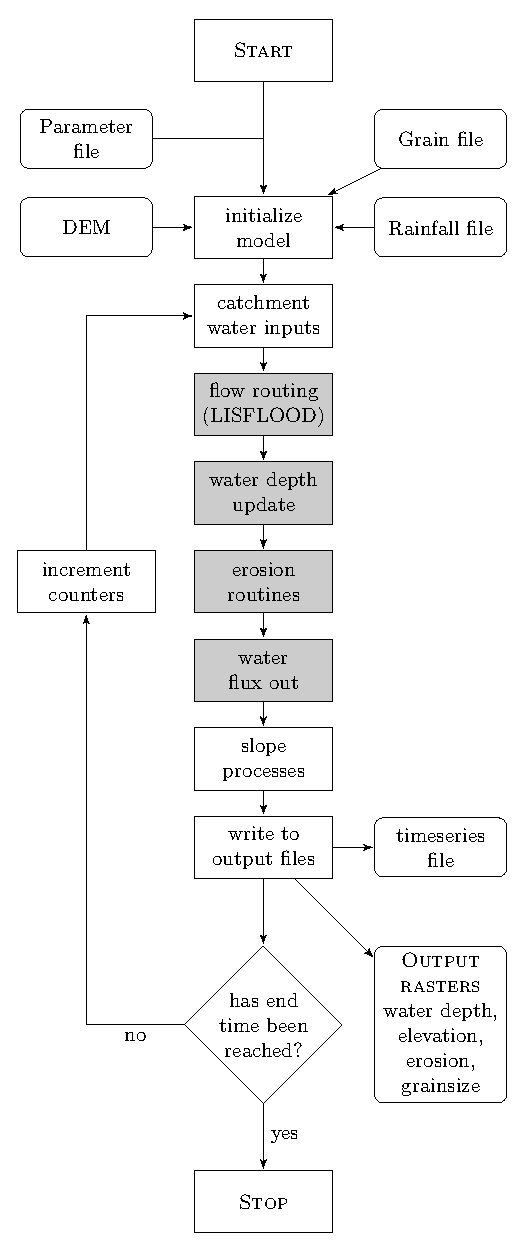
\includegraphics[width=8.3cm]{chp05_figures_scripts/tikz.eps}
\caption{Flow chart showing a simplified outline of the HAIL-CAESAR program flow. Grey shaded boxes indicate sections of the code parallelised with OpenMP. Rounded rectangles indicate output and input files.}
\label{fig_flowchart}
\end{figure}
%\paragraph*{Fully distributed hydrology}
%
%\paragraph*{Interoperability with netCDF data}

\subsection{Process representation}

\subsubsection{Catchment hydrology}

Runoff from rainfall inputs to the catchment is generated using an adaptation of the TOPMODEL hydrological model \citep{beven1979physically}. The TOPMODEL approach first calculates a combined surface and subsurface discharge for the cells within a `wetted' zone of the catchment \citep{coulthard2002cellular}. The wetted cells approach has the advantage of reducing the number of cells that must be scanned every model iteration, lowering computational cost of the model run. When local rainfall rate in a given grid cell is greater than zero, the total runoff, \(Q_{tot}\), for a grid cell is given by: 

\begin{equation}
Q_{tot} = \frac{m}{T} \log \left( \frac{(r-j_t) + \exp \left(\frac{rT}{m} \right)}{r} \right)
\end{equation}
where \(m\) is a parameter that controls the rise and fall of the soil moisture store, \(j_t\), \(T\) is the time step in seconds, and \(r\) the rainfall rate in metres per hour. The soil moisture store, \(j_t\), is given by the formula:

\begin{equation}
j_t = \frac{r}  { \left(  \frac{r-j_{t-1}}{j_{t-1}  } \exp \left( \left( \frac{(0-r)T}{m}\right) +1 \right) \right)}
\end{equation}

\noindent
When rainfall rate is zero during the current iteration, the total runoff, \(Q_{tot}\), is given by the equation:

\begin{equation}
Q_{tot} =  \frac{m}{T} log \left( 1 + \left( \frac{j_t  T}{m} \right) \right)
\end{equation}

\noindent
with the soil moisture store, \(j_t\), given by:

\begin{equation}
j_t = \frac{j_{t-1}}{1 + \left( \frac{j_{t-1}T}{m} \right) }
\end{equation}

\noindent
Total runoff, \(Q_{tot}\), is apportioned between surface and subsurface discharge by a user-set threshold for discharge, \(Q_{min}\). When the volume of water for a given cell exceeds this threshold, it is treated as surface runoff and routed according to the flow routing algorithm described in the following section.

%

\subsubsection{Surface flow routing}
Surface water and channel flow is an important driver of catchment scale erosional processes. The amount and velocity of water flow is a variable in both the sediment transport and bedrock erosion laws. The surface water flow equations are based on a simplified form of the shallow water flow equations, a simplification first derived by \citet{bates2010simple} and later incorporated into the CAESAR-Lisflood landscape evolution model by \citet{Coulthard2013}. The flow between cells is calculated by:

\begin{equation}
Q = \frac{q - g h_{flow} \Delta T \frac{\Delta (h+z) }{\Delta x}}{1 + g h_{flow} \Delta t n^2 |q| / h_{flow}^{10/3}} \Delta x
\end{equation}


\subsubsection{Sediment transport and erosion}
\label{trans_model}

Transport of loose sediment is governed by the \citet{wilcock2003surface} sediment transport model. The Wilcock and Crowe model represents transport of mixed sand/gravel fractions based on the surface sediment composition. The rate of sediment transport, \(q_i\), is given as:

\begin{equation}
q_i = \frac{F_i {U_*}^3 {W_i}^*}{(s -1) g}
\end{equation}

\noindent
where \(F_i\) is the fractional volume of sediment, for a given sediment fraction, \(i\), \(U^*\) is the shear velocity, \(s\) is the ratio of sediment to water density. \({W_i}^*\) is a function relating fractional transport rate to total transport rate \citep[see][for a full derivation of this equation]{wilcock2003surface}. The usage of this sediment transport model is extrapolated here to account for finer particles such as silts \citep{van2007embedding}, as well as the sand-gravel mixture it was originally designed for.

\subsubsection{Bedrock incision}
\label{bedrock_model}
A simple model of bedrock incision based on the excess shear stress model \citep{tucker2001child,tucker2004drainage} is implemented in the numerical model. The rate of bedrock incision is determined by the amount of shear stress acting on the bedrock, above a threshold level of stress required to initiate substrate removal \citep[e.g.,][]{Snyder2003}. When bedrock material is removed, it is distributed amongst the sediment fractions according to the fractional proportions set by the user. The rate of bedrock erosion according to the excess shear stress model is given by:

\begin{equation}
\varepsilon = k_e(\tau_b - \tau_c)^{P_b}
\end{equation}

\noindent
where \(k_e\) is the bedrock erodibility coefficient, \(\tau_b\) is the basal shear stress on the channel bed, \(\tau_c\), is the critical shear stress threshold, \(P_b\) is the shear stress exponent \citep{howard1983channel,whipple1999dynamics}.

\subsection{Parallelisation implementation}
The HAIL-CAESAR code is parallelised using a shared-memory parallelisation model. In brief, the shared-memory technique works by distributing the processing load to multiple processing units that all have access to the same memory address space. The HAIL-CAESAR code uses the OpenMP application programming interface (API), which is widely supported on a range of software platforms and computing architectures \citep{dagum1998openmp}. Shared-memory parallel codes such as the one described in this thesis are suitable for any computing system where the physical processors have access to the same memory space. A wide range of systems can avail of shared-memory parallel codes, from multi-core desktop computers, through high-end multi-processor, multi-core workstations, to individual compute nodes on high performance computing services (HPC). The code presented has been tested on a wide range of architectures including desktop computers,  small-scale cluster computing facilities, and national scale HPC services.

The main functions in the program that are parallelisable, and most computationally expensive, are the water routing algorithm (\textit{flow\_route}), the erosion routines (\textit{erode}), the water depth update function (\textit{depth\_update}), and the catchment wetted-area scanning function (\textit{scan\_area}). These were identified by profiling the serial version of the code using the \textit{gprof} profiling tool \citep{graham1982gprof}, and the results are shown in Tables \ref{profile_speed_up_hydro} and \ref{profile_speed_up_erode}. Initially, it may appear that using a wetted-cells approach with the \textit{scan\_area} function would be a counter-intuitive way to reduce computation time, as the \textit{scan\_area} function is computationally expensive itself. However, preliminary experimentation with removing the \textit{scan\_area} function (and scanning all cells in the catchment every iteration) showed that in fact the computational expense of calling this function was far outweighed by the large reduction in cells that had to be scanned every iteration. In practice this is likely due to the fact that catchments are rarely inundated totally, even during flood events, as only the floodplains maintain a significant depth of water. The number of wetted cells is therefore likely to be much smaller than the total number of grid cells in the model domain for the majority of cases, and the wetted cell scanning function (\textit{scan\_area}) overall reduces computation time.

\begin{table}
\caption{Summary of most expensive program functions, using a test case of a 48 hour flood simulation, with the model run in \textbf{hydrology-only mode}. The test case is based on the flooding that took place in the Boscastle (River Valency) catchment in August 2004, in Cornwall, UK \citep{golding2005boscastle}.}
\begin{tabular}{cl}
%\multicolumn{2}{c}{\textbf{Profiling results of 48 hour simulation in hydrological mode}} \\

\textbf{Time} (percentage of total) & \textbf{Function name} \\
\hline
77.71                                     & flow\_route \\
17.63                                     & depth\_update \\
3.58                                       & scan\_area \\
1.02                                       & catchment\_waterinputs \\
0.03                                       & water\_flux\_out \\
\hline \\
\end{tabular} 
\label{profile_speed_up_hydro}
\end{table}

\begin{table}
\caption{Summary of most expensive program functions, \textbf{with erosion processes enabled}, using a test case of a 48 hour flood simulation. The test case is based on the flooding that took place in the Boscastle (River Valency) catchment in August 2004, in Cornwall, UK \citep{golding2005boscastle}.}
\begin{tabular}{cl}
%\multicolumn{2}{c}{\textbf{Profiling results of 48 hour simulation in erosion-enabled mode}} \\

\textbf{Time} (percentage of total) & \textbf{Function name} \\
\hline 
37.96                                    & erode \\
25.68                                     & flow\_route \\
15.90                                       & scan\_area \\
11.47                                      & depth\_update \\
3.75                                    & (matrix library functions) \\
1.84                                       & d50 \\
1.63                                       & slide\_GS \\
0.59                                      & sort\_active \\
0.46                                      & catchment\_waterinputs \\
0.20                                     & sand\_fraction \\
\hline \\
\end{tabular} 
\label{profile_speed_up_erode}
\end{table}


\paragraph*{flow\_route}
The \textit{flow\_route} function is the core water-routing algorithm based on the \citet{bates2010simple} algorithm. The \textit{flow\_route} function accounts for c. 26\% of compute time in a typical erosion-enabled simulation, and 78\% of compute time in a flow-only simulation.  As one of the most compute-intensive sections of code when the catchment is in flood, the parallelisation of this section achieved significant overall code speed up for a variety of data inputs. The flow routing algorithm is only performed on those cells in the model domain that have accumulated a water depth, i.e. it is not performed in `dry' cells. This means that only a small subset of cells are accessed during the flow routing section of the code, given a typical scenario where there are significant amounts of flow in the channels and floodplain areas, but little or none on the hillslopes. The code and parallelisation of the \textit{flow\_route} function is given in outline form below:

\begin{verbatim}
#pragma omp parallel for
    schedule(runtime)
for (int y=1; y<=jmax; y++)
{
  int inc = 1;
  while (down_scan[y][inc] > 0)
  {
  // Water routing in x direction...
  
  // Water routing in y direction...
  inc++;
}
\end{verbatim}

\paragraph*{depth\_update}
Profiling of the serial code identified the water depth update function as being one of the most compute intensive parts of the code for hydrology-only and erosion-enabled simulations. Updating of water depths is done using the same scanning algorithm as described for \textit{flow\_route}, updating depths in cells where there is water, or in neighbouring cells to water-containing cells. An outline of the implementation is presented below:

\begin{verbatim}
#pragma omp parallel for 
     reduction(max:l_maxdepth)
     schedule(runtime)
for (unsigned y = 1; y<= jmax; y++)
{
  int inc = 1;
  double tempmaxdepth = 0;
  while (down_scan[y][inc] > 0)
  {
    // Update water depths
    // Update suspended sediment 
    //   concentrations
    // Calculate maximum flow depth
    ...
    inc++;
  }
}
\end{verbatim}

\paragraph*{scan\_area}
The \textit{scan\_area} function analyses the catchment to determine which cells contain water or neighbour water-containing cells and sets an index array based on the current wetted area of the catchment. Further functions that involve updating sediment or water transport amounts then use this array as a mask so that only catchment model cells that contain water will be inspected and have their sediment and water totals updated.
\begin{verbatim}
#pragma omp parallel for
for (int j=1; j <= jmax; j++)
{
  int inc = 1;
  for (int i=1; i <= imax; i++)
  {
    // zero down_scan array
    down_scan[j][i] = 0;
    // and work out scanned area. 
    if (water_depth[i][j] > 0
        || water_depth[i][j - 1] > 0
        || water_depth[i][j + 1] > 0
        || water_depth[i - 1][j] > 0
        || water_depth[i - 1][j - 1] > 0
        || water_depth[i - 1][j + 1] > 0
        || water_depth[i + 1][j - 1] > 0
        || water_depth[i + 1][j + 1] > 0
        || water_depth[i + 1][j] > 0
        )
        {
        down_scan[j][inc] = i;
        inc++;
        }
    }
}
\end{verbatim}

\paragraph*{erode}
The most compute-intensive part of the code when run in erosion-enabled mode is the \textit{erode} function. This function performs all sediment entrainment and transport routines. The serial-run test simulation spent c. 38\% of its time in this function, plus an additional 5\% of time in function calls within the main \textit{erode} routine. 

\begin{verbatim}
#pragma omp parallel for 
    reduction(max:tempbedloadmax) 
    schedule(runtime) 
for (unsigned int y = 1; y < jmax; ++y) 
{
  int inc = 1;
  while (down_scan[y][inc] > 0)
  {
    unsigned x = down_scan[y][inc];
     inc++;
     // Calculate sediment entrainment
     ...
   }
}

#pragma omp parallel for
{
  // Sediment transport in x-direction
}

#pragma omp parallel for
{
  // sediment transport in y-direction
}

#pragma omp parallel for
{
  // Calculate sediment transport
  //   from all 4 edges
  // of the model domain
}

\end{verbatim}


\subsection{Potential speed up from parallelisation}

The functions described above, \textit{flow\_route, depth\_update, scan\_area,} and \textit{erode}, account for 98\% and 94\% of the compute-time in hydrology-only and erosion-enabled modes, respectively. The model is profiled using a 48 hour test simulation of a flash flood event in the summer of 2004 in the UK, referred to as the `Boscastle' simulation. (Full details of this flood event are described in Chapter \ref{chapter_events}.) Effective parallelisation of the compute-time dominating functions should result in effective parallel speed-up. The potential speed-up as a result of parallelisation can be estimated using Amdahl's law \citep{amdahl1967validity}. The law gives the predicted speed up on \(N\) processing units based on ideal scaling over multiple cores. Ideal parallel speed-up, \(S\) is given by:

\begin{equation}
S = \frac{1}{(1-P)+(P/N)}
\label{eqn_amdahl}
\end{equation}

\noindent
where \(P\) is the proportion of program time that can be run in parallel. (Note that \(P\) may vary slightly between simulations, based on the input data and certain model parameters supplied to the program.) Profiling the program with the Intel VTune amplifier performance analysis tool suggests that the program spends 94\% of its time in parallel sections of the code during an erosion-enabled simulation and 98\% of compute-time in parallel sections during a hydrology-only simulation. Using Amdahl's law it is possible to calculate theoretical potential speed-up given in Table \ref{Amdahl_table}. At the maximum available processor count of 48 cores, speed ups of up to c.20 times are predicted for a hydrology-only simulation, and up to c.13 times for an erosion-enabled simulation. The limitations of Amdahl's law are that it predicts only idealised speed ups, and does not account for any overheads in parallelisation, such as the creation and synchronisation of threads, nor does it account for performance issues due to the speed of memory access in memory-bound computational problems \citep{hill2008amdahl,sun2010reevaluating}.

\begin{table}
\caption{Idealised potential speed-up according to Amdahl's law (equation \ref{eqn_amdahl}). Value for \(P\) calculated using profiling results from the Boscastle (River Valency) flood test simulation after 48 hours simulated time.}
\begin{tabular}{ccc}
%\multicolumn{3}{c}{\textbf{Idealised parallel speed-up}} \\ 
\textbf{Number of CPUs} & \textbf{Speed-up} (Hydro) & \textbf{Speed-up} (Erosion) \\

 & \(P=0.98\) & \(P=0.94\) \\
\hline 
2 & 1.94 & 1.89  \\ 
4 & 3.67 & 3.39  \\ 
8 & 6.11 &5.63  \\ 
16 & 11.03 & 8.42 \\ 
32 & 16.58 & 11.2 \\ 
48 & 19.92 & 13.4 \\ 
\hline \\
\end{tabular}

\label{Amdahl_table} 
\end{table}



\section{Testing and benchmarking}

Two aspects of model performance are tested in this section. Firstly, tests are carried out to verify that the HAIL-CAESAR model produces comparable scientific results with that of its progenitor, CAESAR-Lisflood. Secondly, benchmarking tests are done to measure any performance gains of HAIL-CAESAR arising from its implementation in C++, parallelisation strategy, and choice of compiler. The HAIL-CAESAR model is tested with two different compilers, to assess any potential differences arising from the choice of compiler. These are the \textit{GCC (GNU compiler collection)} C++ compiler and the \textit{Intel} C++ compiler. The CAESAR-Lisflood model is supplied already compiled with the Microsoft \textit{MSVC} C\# compiler. In all cases, compiler optimisation flags are turned on for the compilation process.

\subsection{Regression testing}

Regression testing is a software development practice used to verify that software that has been modified, interfaced with other software, or re-implemented, still performs as expected when compared to the original implementation \citep{wong1997study}. To verify that HAIL-CAESAR produces comparable results to the original CAESAR-Lisflood model, a set of simulations with the same test data and input parameters for both models is carried out. The catchment hydrological and sediment outputs from a 10-year simulation of the River Swale, North Yorkshire, United Kingdom are compared for consistency between both implementations. The Swaledale test case has been well calibrated in previous studies \citep[e.g.,][]{Coulthard2001} and is supplied with the original CAESAR-Lisflood model as a standard test case. Details of the model testing simulations are shown in Table \ref{versus_CL}. 

Three metrics are used to compare the two models (and choice of compiler in HAIL-CAESAR): water discharge rate from the catchment outlet, hourly sediment output, and cumulative sediment output from the catchment over the course of the simulation. 
Figure \ref{fig_swale_regression_lisflood} shows the differences in water discharge comparing HAIL-CAESAR with the original CAESAR-Lisflood model. (For clarity, only the first 250 days are shown.) The flow routing algorithm performs similarly in both models, with the largest discrepancies seen in the first 100 days. An inset in Figure \ref{fig_swale_regression_lisflood} shows the typical magnitude and timing of differences in the discharge. The timing and magnitude of the largest flood peaks are comparable, and the largest differences in magnitude on the order of 1--10 \(m^3s^{-1}\).
Figure \ref{fig_swale_regression_sediment} shows the sediment flux from the catchment outlet. While there is low-magnitude variation in the sediment flux signal, the main peaks in sediment discharge are at similar times and of similar magnitude in both implementations. Figure \ref{fig_swale_regression_cum_sediment} shows the cumulative sediment output from the catchment. Initially, both implementations show close agreement, until approximately 700 days into the test simulation where the predicted sediment totals begin to diverge. The CAESAR-Lisflood implementation, in this case, predicts an overall lower total sediment discharge over the 10-year period. The HAIL-CAESAR implementation predicts c. 40\% greater total sediment yields after 10 years.

\subsection{Differences in sediment flux and yields between models and compilers}

Several factors may explain the small differences seen between the sediment outputs of the two models (HAIL-CAESAR vs CAESAR-Lisflood) and also in the comparison between the two compilers used to test HAIL-CAESAR. The sediment flux differences are shown in detail for first 250 days of the Swale test simulation in Figure \ref{fig_swale_regression_sediment}.

Firstly, floating point numbers cannot be represented exactly in computer memory, due to a finite amount of memory or `bits' that may be used to store each number. In the case of these tests, a \textit{64-bit} data type is used to store numbers. Many calculations using real numbers will produce a result that cannot be represented in the finite number of bits provided by the system ($10 \div 3$, for example, results in 3.333333..., which cannot be stored precisely in a 64-bit data type, or indeed any finite-length data type). Many results such as this must therefore be rounded to fit back into their finite representation \citep{goldberg1991every}. The rounding error is a characteristic feature of floating-point arithmetic performed by computers. Multiplied over thousands or millions of calculations or iterations of the model, initial error can multiply over time and result in small but noticeable discrepancies within results. 
Secondly, optimizing compilers are free to evaluate expressions in a different order, so long as it can be shown the optimisation would produce the same mathematical result. However, this does not guarantee that two compilers will produce the exact same \textit{numerical} result, since many floating point calculations do not have an exact result that can be represented with finite precision. If different compilers optimise calculations to be done in different orders, rounding errors may creep into the results at different stages of the calculation, resulting in slightly different final results \citep{goldberg1991every,monniaux2008pitfalls}.

Optimisation in compilers can be switched off, and it is possible to force compilers to produce bit-for-bit comparable results, however this results in a significant performance drop in simulation times. Given the relatively small size of the numerical error shown in Figure \ref{fig_swale_regression_sediment} between the two models and the different compilers, it was not felt warranted to reduce performance significantly to produce exactly comparable sediment fluxes over these timescales.

The effect of compiler and software system choice on the results from numerical models has also been observed in atmospheric models, where different optimisation techniques performed by different compilers resulted in small discrepancies between otherwise identical simulations using models compiled with different compilers. \citep{hong2013evaluation}. 

Figure \ref{fig_swale_regression_cum_sediment} shows the cumulative sediment totals over a longer ten-year simulation, which although initially are very close matching across model implementation (HAIL-CAESAR vs CAESAR-Lisflood) and compiler choice for HAIL-CAESAR, a divergence between the HAIL-CAESAR results and the CAESAR-Lisflood results appears around the 750 day mark. The results here would indicate the while HAIL-CAESAR and CAESAR-Lisflood produce comparable results for simulations $<$ 750 days, at longer timescales the differences begin to diverge, producing up to  40\% difference after 10 years of simulated sediment output. This again is likely at least partly due to compiler differences producing inexact numerical results. \citet{hong2013evaluation} also find that software system differences produce greater error over longer simulation times, with atmospheric model runs diverging after several days given identical starting conditions but different compiler optimisations. It is believed that a similar effect is evident here. 
Since the scope of this thesis is to investigate small-scale events at short timescales on the order of days, the diverging results at longer timescales were not deemed to be of great concern for the purpose of this study. Good agreement was found between the two models at much shorter timescales, which is sufficient for this study. However, future work on the HAIL-CAESAR model would ideally investigate these discrepancies further.

A detailed analysis of the differences between the C\# compiler used for CAESAR-Lisflood and the Intel and GCC compilers used for HAIL-CAESAR is beyond the scope of this study, but compiler difference remains the most likely source of numerical error based on previously reported study \citep{hong2013evaluation} and established knowledge regarding numerical error in using floating-point arithmetic \citep{goldberg1991every,monniaux2008pitfalls}.

\begin{sidewaysfigure*}[t]
\includegraphics[width=25cm]{chp05_figures_scripts/lisflood_regerssion_new_colours13.png}
\caption{Water discharge rates over first 250 days of simulation. Outputs from the Swale 10 year at 50m resolution test case, showing results from the original CAESAR-Lisflood model and HAIL-CAESAR model compiled under two different compilers: Intel and GCC. The inset highlights the typical magnitude of difference in water discharge where the hydrographs diverge.}
\label{fig_swale_regression_lisflood}
\end{sidewaysfigure*}

\begin{sidewaysfigure*}[t]
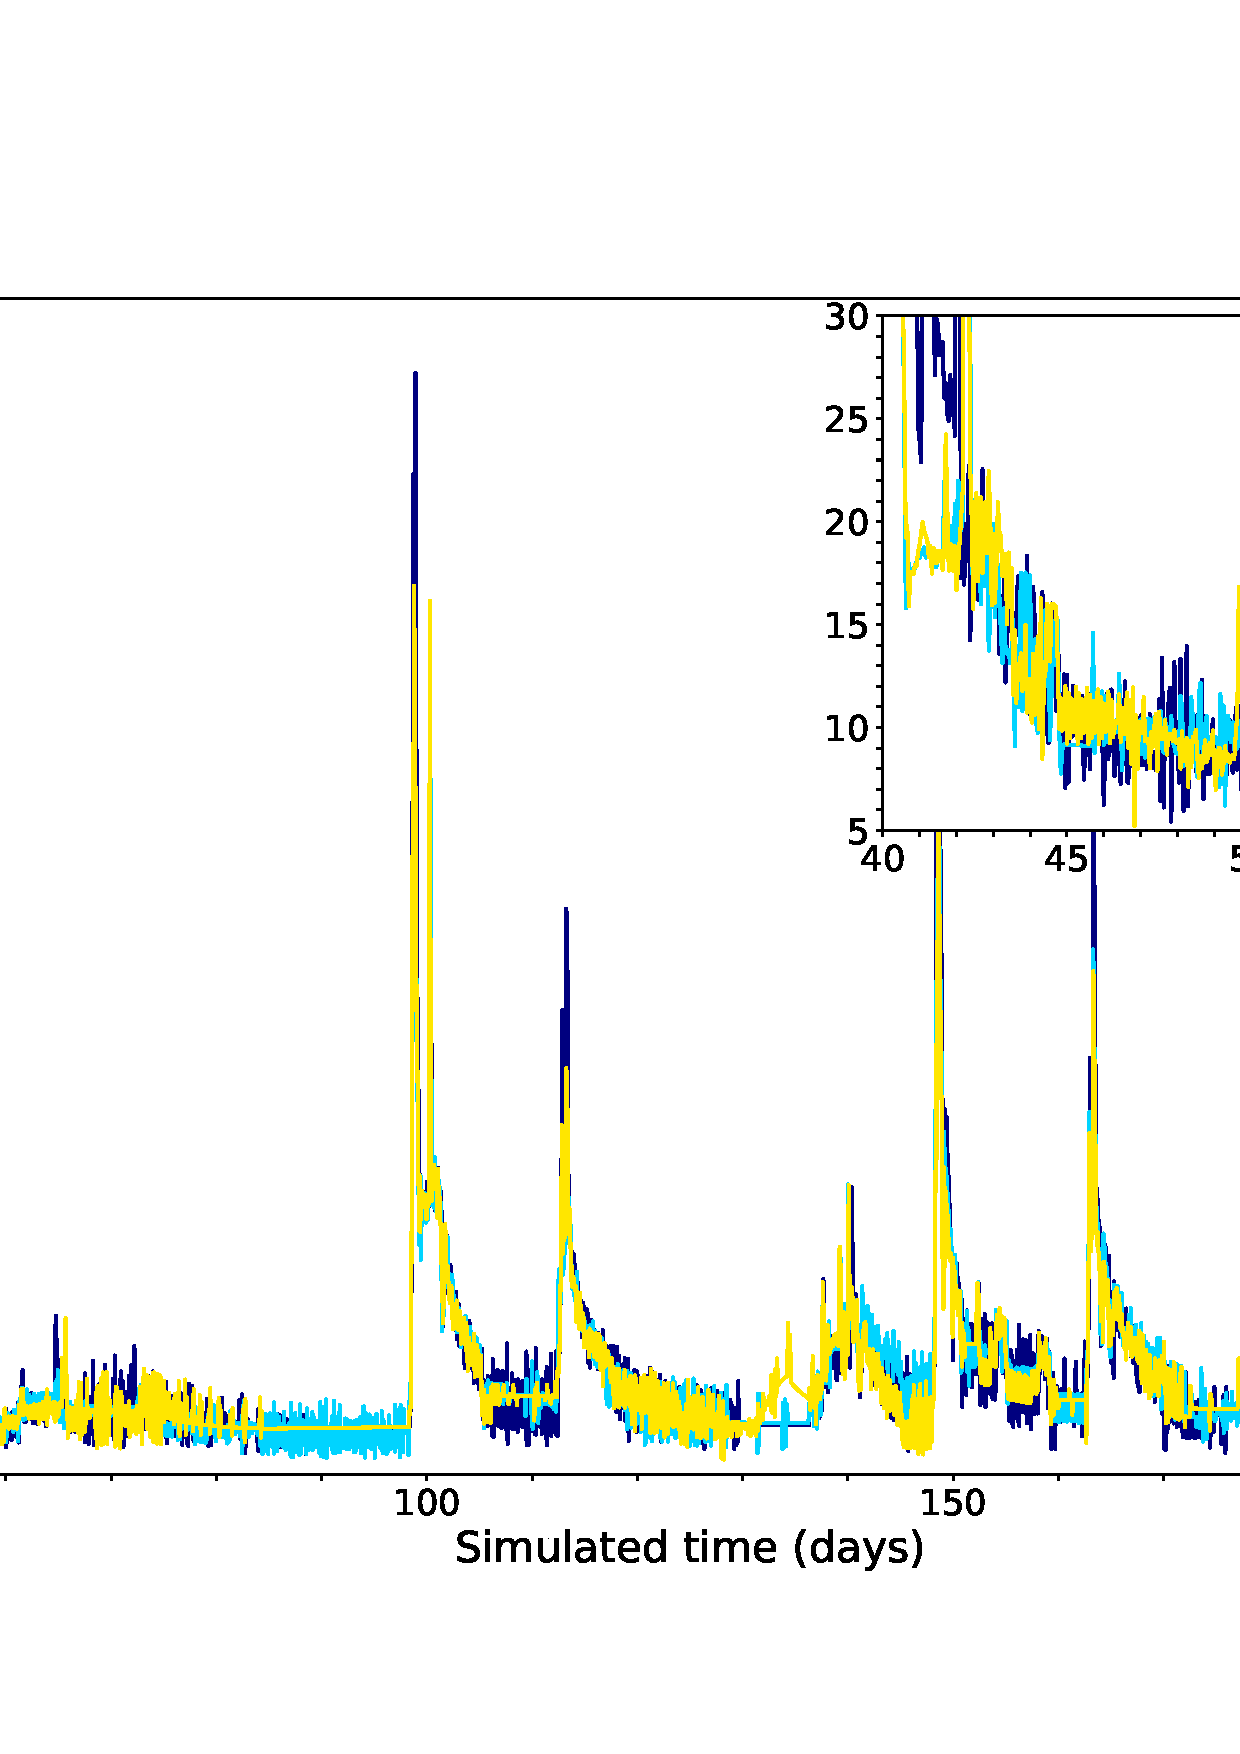
\includegraphics[width=25cm]{chp05_figures_scripts/sed_tot_regression_alpha.png}
\caption{Catchment sediment flux over first 250 days of simulation. Outputs from the Swale 10 year at 50 m resolution DEM test case, showing results from the original CAESAR-Lisflood model and HAIL-CAESAR model compiled under two different compilers: Intel and GCC. The inset is to highlight the typical magnitude in sediment flux difference where the outputs diverge.}
\label{fig_swale_regression_sediment}
\end{sidewaysfigure*}

\begin{figure}[t]
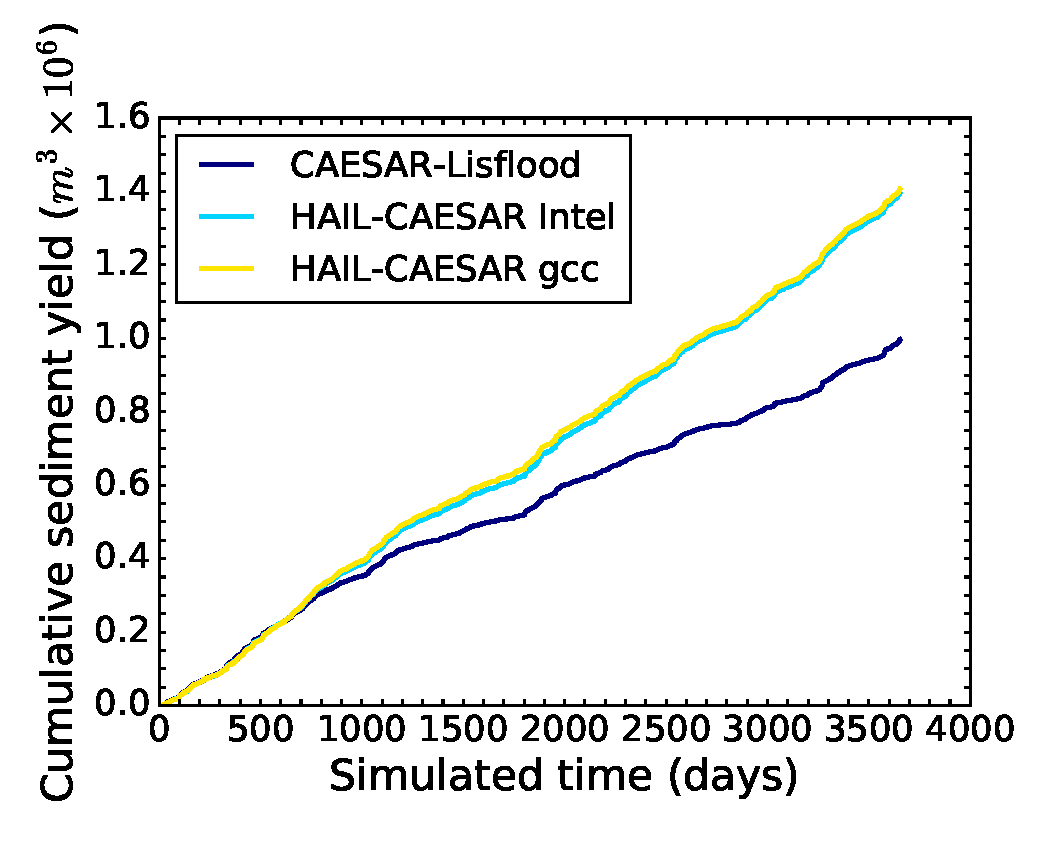
\includegraphics[width=15cm]{chp05_figures_scripts/cum_sed_tot_regression.eps}
\caption{Cumulative catchment sediment flux over full duration of simulation. Outputs from the Swale 10 year at 50 m DEM resolution test case, showing results from the original CAESAR-Lisflood model and HAIL-CAESAR model compiled under two different compilers: Intel and GCC.}
\label{fig_swale_regression_cum_sediment}
\end{figure}

\subsection{Performance comparison with CAESAR-Lisflood}

Though the code base of HAIL-CAESAR and CAESAR-Lisflood differ somewhat, due to differences in implementation detail between the C\# and C++ languages, as well as the parallelisation libraries used, the underlying algorithms remain broadly the same. The two models were compared on similar hardware to assess any gains in speed-up from porting the CAESAR-Lisflood model to a C++ implementation using the OpenMP parallelisation libraries.

The hardware used for this test study was a workstation computer with an Intel i7 8-core processor and 32GiB of memory. The CAESAR-Lisflood test simulations were run on a Windows operating system, as per the requirements of the software; the HAIL-CAESAR model test simulations were run on a Linux operating system on the same machine. The input parameters and input DEM were kept the same for all benchmarking simulations. The details of the test case configurations are shown in Table \ref{versus_CL}.

Using the HAIL-CAESAR implementation, a speed up of c.41\% was seen using the open-source GNU C++ compiler (gcc) and a speed-up of 48\% using the Intel C++ compiler. As the core algorithms remain the same in both versions of the code, the speed up likely comes from the fewer overheads in the command-line based HAIL-CAESAR model, and potentially through better compiler optimisations available with the C++ compilers. Further speed up may come from the fact that the CAESAR-Lisflood model is executed through a \textit{just-in-time} compiler, translating pre-compiled bytecode into machine code at runtime \citep{aycock2003brief}. In contrast, HAIL-CAESAR runs using a compiled binary executable file, with machine code generated at compile time. The HAIL-CAESAR approach avoids the potential overheads of invoking the dynamic compilation stage in C\#/.NET programs.

\begin{table*}


\resizebox{\textwidth}{!}
{%
\begin{tabular}{cccc}
%\multicolumn{4}{c}{} \\
Model Version & \textbf{CAESAR-Lisflood 1.9b} & \multicolumn{2}{c}{\textbf{HAIL-CAESAR v1.0}} \\
\hline \\
Runtime (hrs:mins) & 7:00 & 4:09 & 3:39 \\
Programming Language & C\# & C++ & C++ \\
Compiler & MSVC 14.0 & GCC 6.2 & Intel v17.0 \\
Optimisation flags & -optimize & -O3, -march=native & -O3, -march=native \\
Parallel library & C\# native parallel library & OpenMP 4.5 & OpenMP 4.0 \\
Processor & \multicolumn{3}{c}{Intel i7-3770 8 core @ 3.4GHz, 32GiB memory} \\
\hline \\
\end{tabular} 
}
\caption{Initial performance and compilation comparison with CAESAR-Lisflood, using the River Swale test case, 50m DEM, 10 year simulation} 
\label{versus_CL}
\end{table*}

\subsection{HPC profiling and speed-up}

\subsection{Performance scaling on HPC compute nodes}
The primary aim in developing this software was to have a code that ran on Unix-based high performance computing systems and could be re-compiled for a variety of different platforms and computer architectures. This section demonstrates the scaling potential and optimal hardware configurations using a single compute node on a typical HPC system. Test simulations are run on the ARCHER supercomputer. Each compute node consists of a two Intel Ivybridge Xeon processors, each with 12 cores per physical processor. Simultaneous multi-threading allows each core on the processor to effectively act as if it were two separate processing units, giving a total of 48 possible threads/cores per compute node. A single compute node consists of two NUMA\footnote{Non-uniform memory access}-regions each with access to 16GiB of memory, a total of 32GiB per compute node. 

\subsection{Strong scaling}
Strong scaling describes how the performance increase of the code scales as more processors are used to solve a problem of fixed size. We test two typical use case scenarios for the HAIL-CAESAR model. The first case is an extension of the standard test case using the Swale data. The use of the model in this case is typical of longer duration landscape evolution simulations, with periods of predominantly low hydrological flows interspersed with brief (relative to the simulation time) storm events. The second case uses the HAIL-CAESAR model to simulate a single storm event at higher spatial resolutions, over a much shorter timescale. Two contrasting model applications are chosen to represent the range of timescales the model can be applied to, from short term single storm events to annual and decadal simulations. The simulations are all run with spatially uniform rainfall input.

\begin{table}
\caption{Strong scaling test cases used to benchmark the HAIL-CAESAR model, using Swaledale and Boscastle DEMs.}
\begin{tabular}{ccccc}
\\
\multicolumn{5}{c}{\textbf{Strong scaling benchmarking simulations}} \\
\hline 
Catchment & Swaledale & \multicolumn{3}{c}{Boscastle} \\
Grid cells & 124931 & \multicolumn{2}{c}{720000} & 4500000 \\ 
DEM cell size & 50m & 5m & 5m & 2m \\ 
Simulation time & 8670 hrs & 48 hrs & 72 hrs & 72 hrs \\ 
Catchment Size & 150km$^2$ & {12km$^2$} & {12km$^2$} & {12km$^2$} \\ 
Number of cores & \multicolumn{4}{c}{1, 2, 4, 8, 16, 20, 30, 36, 40, 48} \\ 
\hline \\
\end{tabular} 
\label{strong_scale_table}
\end{table}

\paragraph*{Multi-event simulation, 1 year}
The Swaledale test case is run over a 1 year duration, using an input DEM of 50 m resolution. The model is run in hydrology-only and erosion-enabled modes. The input parameters and input DEM are the same for each simulation, as each simulation is repeated on an increasing number of processors (Table \ref{strong_scale_table}). At the maximum core count of 48 core, results from this simulation show speed up of up to 700\% and 550\%, for erosion-enabled and hydrology-only modes, respectively. The speed-up shown for erosion-enabled simulations does not always increase in concert as core-counts are increased, although the overall trend is one of increasing speed-up. For example, erosion-enabled simulations with 16, 24, and 36 processors showed a slow down when compared to the preceding benchmark tests using 12, 20, and 30 processors, respectively (Figure \ref{fig_strong_scale_multi}). The hydrological-only simulations showed a more consistent speed-up between benchmark tests (Fig. \ref{fig_strong_scale_multi}), though speed-up potential begins to decline at thread counts around 30 threads and higher, where it is observed the gains from increasing the thread count further diminish.

\paragraph*{Single-event simulation, 48--72 hours}

For this benchmark, two sets of strong scaling experiments are done with two different resolution DEMs. For each set of experiments, the input terrain data and parameters remain the same while increasing the number of processors over which the problem is shared. The strong scaling benchmark tests use a model domain with a) 720 000 grid cells, and b) 4 500 000 grid cells, representing a 12km$^2$ river catchment with 5m and 2m resolution DEMs, respectively. At this resolution of DEM, it possible to resolve the larger channel geometries at the grid-scale, without resorting to techniques of `burning in' the DEM with a channel. Sub-grid parameterisation of the channel shape, a feature of some models, is also not required.

Since HAIL-CAESAR features both a flood-inundation-only and sediment erosion mode, two further sets of benchmarks were done for both problem sizes, one with the model running in hydrology-only mode, and another running in the erosion-enabled mode.

The results from the single-event scaling benchmark show the greatest speed-up for the 48 hour Boscastle simulation, with a speed-up of almost 16 times at 48 threads/cores, for the hydrology-only simulation. Erosion-enabled simulations also show food speed-up for this problem size (720 000 grid cells), but the linear speed-up trend is lost above around 30 cores, when speed-up gains begin to tail-off. At the larger problem size of 4 500 000 grid cells, the speed-up gains from increasing core counts is much diminished, though still increases linearly through higher core counts. Speed-up here reaches only about 5 times running on 48 cores, in hydrology-only mode, and 3.5 times in erosion-enabled mode.

\begin{figure}[t]
\includegraphics[width=11cm]{chp05_figures_scripts/strong_scale_four.eps}
\caption{Speed-up achieved relative to serial code on 2, 4, 8, 12, 16, 20, 24, 30, 36, 42, and 48 cores. Four sets of simulations are used representing a range of model uses from short, single event episodes (48--72hr) to 1 year simulations.}
\label{fig_strong_scale_multi}
\end{figure}

\subsection{Weak scaling}

Weak scaling is a parallel performance metric used to assess how the code runtime scales as the amount of work per processor is kept the same, but the total problem size -- in this case, the number of grid cells in the model domain -- is increased \citep{gustafson1988reevaluating}. This mirrors the practice of using larger numbers of processors to tackle model simulations using higher resolution topographic data, or data covering a larger spatial domain. The weak scaling experiments used a set of hydrology-only simulations and a set of erosion-enabled simulations. A series of 72 hour simulations were done using a range of high-resolution topographic datasets, from 0.5 m to 5 m resolution, scaling the number of processors used to maintain the ratio of processors/workload as near as possible. The number of model domain grid cells per core was fixed at approximately 1 500 000. The simulations were repeated for hydrological-mode and erosion-enabled modes, but due to the high memory demands of running very high resolution erosion-enabled simulations, not all simulations could be completed on the available hardware, which has a maximum job runtime of 48 hours.

The simulations in hydrological-only mode show positive weak scaling as the problem size increases in tandem with the number of threads (Figure \ref{fig_weak_scale}). Ideal weak scaling would be expected to show a runtime per number of grid cells/cores remaining approximately constant compared with a single-threaded simulation. The slight increase seen in the weak scaling here is likely due to the overheads experienced with creating and synchronising the extra threads as the problem size is increased.

\begin{sidewaystable*}[t]
\caption{Weak scaling test cases with the Boscastle DEM resampled at increasing resolutions from 0.5m to 5m. The absence of run-time results for certain erosion simulations is due to memory limitations preventing higher resolution simulations from running.}
\resizebox{\textwidth}{!}
{%
\begin{tabular}{ccccccc}

\multicolumn{7}{c}{\textbf{Weak scaling simulations, Boscastle DEM, 72 hour simulation}} \\ 

DEM resolution (m)  &  Grid cells & Ideal no. of threads & No. of threads & Cells per thread & Run time (Hydro) & Run time (Erosion) \\ 
\hline
0.5 & 72 000 000 & 48    & 48 &  1 500 000 & 323.1 & --  \\
0.6 & 49 900 050 & 33.3 & 33 &  1 512 122 & 190.4 & -- \\
0.7 & 36 808 200 & 24.5 & 26 &  1 472 328 & 138.8 & -- \\
1.0 & 18 000 000 & 12    & 12 &  1 500 000 & 84.3 & 355.2 \\
1.5 & 7 960 050   & 5.3   &  5  &   1 592 010 & 49.0 & -- \\
2.0 & 4 500 000   & 3      &  3  &   1 500 000 & 568.9 & 1112.1 \\
5.0 & 720 000      & 0.48 & 1  &    720 000 & 347.306 & 432.3 \\ 
\hline \\
\end{tabular} 
}
\label{weak_scale_table}
\end{sidewaystable*}

\begin{figure}[t]
\includegraphics[width=11cm]{chp05_figures_scripts/weak_scale_bos.eps}
\caption{Weak scaling with the Boscastle DEM at increasing resolution (see Table \ref{weak_scale_table}). Hydrological and erosion-enabled simulations shown. Each simulation uses c.150 000 grid cells per CPU. The absence of results for certain erosion simulations is due to memory limitations preventing higher resolution simulations from running.}
\label{fig_weak_scale}
\end{figure}


%\subsubsection{Compiler influence}
%
%The influence of compiler choice on performance is investigated using three compilers: gcc v5.1, Intel vX, and the Cray compiler vX.X.
%
%\subsubsection{Optimisation options}

\subsection{Thread profiling}

Further profiling of the parallelised version of the code was carried out using the Intel\textregistered \ VTune Amplifier performance analyser. Thread profiling shows where the bottlenecks in the code are, including functions that are compute intensive, but also where inefficiencies occur due to overheads from parallelisation and load imbalance. For clarity, a single example using the Boscastle test case is presented, with a simulated model time of 48 hours, running on 8 cores/threads. It is expected that different simulations and domain sizes would produce slightly different results, but this simulation gives a general idea of the parallel performance of specific functions in the code.

The break down of major function overheads is shown in Figure \ref{fig_thread_profile}. Only four of the key parallel-implemented functions, \textit{erode, flow\_route, scan\_area,} and \textit{depth\_update} are assessed, as other functions collectively amounted to a small proportion of the runtime, or were serial functions. Load imbalance accounts for 22\% of the execution time of these four key functions, due to certain threads sitting idle while waiting for other threads to complete. Load imbalance is particularly apparent in the \textit{erode} and \textit{depth\_update} functions. Overhead time (from the creation and synchronisation of threads) is minimal across all functions. The issue of load imbalance is discussed further in Section \ref{sec_loadbalance}.

\begin{figure}[t]
\includegraphics[width=11cm]{chp05_figures_scripts/fig_thread_profile.eps}
\caption{Thread profiling of the Swale 1 year simulation with 50m DEM. Data from major functions only displayed.}
\label{fig_thread_profile}
\end{figure}

%\subsection{Ensemble simulation potential on HPC clusters}
%
%The growing availability of HPC services has been thus far seldom exploited by the geomorphic and landscape evolution modelling community. This section briefly explores the potential for using such computing services to run ensemble simulations of landscape evolution models, using the HAIL-CAESAR model and Swale test case used in previous sections. The ARCHER HPC service is used for the test simulations. 

\section{Discussion}

%Strong scaling
%weak scaling
%Problem-type and size dependency
%Load-balancing issue
%Scheduling

\subsection{Parallel scaling}
%Strong scaling
%weak scaling
%Problem-type and size dependency
There are three factors that potentially affect the parallel scaling observed in the benchmarking test cases presented. 
\begin{enumerate}
\item The number of grid cells in a model domain, i.e. the total problem size, which is dependent on the resolution of the DEM input data. 
\item The choice of running the simulation as hydrology-only or erosion-enabled model. The erosion option in the model also increases memory demands significantly compared to the hydrology-only mode, as well as computational expense.
\item The hydrological state of the catchment. When the catchment is experiencing flooding due to high rates of rainfall input, the number of cells registered as containing water through the \textit{scan\_area} algorithm increases substantially. The location of the water-containing cells in a catchment also determines the amount of load-imbalance in the model. If water-containing cells are concentrated only in a certain area of the catchment, significant load-imbalance will occur. 
\end{enumerate}

The most favourable speed-up was observed in the Boscastle 48 hour simulation at 5 m DEM resolution (Figure \ref{fig_strong_scale_multi}.) A speed-up of almost 16x was recorded using the maximum number of cores available on the test hardware. Increasing the length and resolution of the Boscastle simulation appeared to negatively affect the speed-up potential of the simulation. Speed-up gains remained approximately linear into higher core counts, with slight tail-off in speed-up gains observed when approaching 48 cores. The longer-term Swale simulation exhibited poorer scaling, with a gradual drop in speed-up gains as the number of threads/cores was increased. 

There is not a clear relationship between number of grid cells in the model domain and speed-up potential. The Swale test case (about 125 000 grid cells), for example, showed almost half as much speed up as the 48 hour Boscastle simulation, despite the latter having 720 000 grid cells in the model domain. 

The enabling of erosional processes in simulations did not significantly affect the scaling potential of the simulations. Most benchmark results showed slightly less favourable speed up at higher core counts for erosion-enabled simulations, but this did not appear to be the controlling factor on scaling. In one case (Swale) the erosion-enabled simulation ran 2x faster than the corresponding hydrology-only simulation. The lack of contrast between erosion-enabled and hydrology-only simulations may be explained by the adpative time stepping feature used in the \textit{erode} function. In erosion-enabled mode, the timestep increases substantially during periods of low water flow and erosion rates, and this may offset the increased computational demands from the \textit{erode} function.

The Boscastle and Swale test cases represent different types of catchment hydrological state. The Boscastle simulations essentially represent a single intense flooding event, where the catchment is in a period of low flow followed by an intense burst of rainfall and erosion for a few hours. The Swale simulation represents a series of storm events, interspersed with `dry' periods, where the model will be able to increase the timestep, but not make heavy use of parallel sections of the code reserved for water routing and erosion routines. 

\subsection{Load balancing issues}
\label{sec_loadbalance}
Parallel computing problems in which the distribution of workload between each thread or processor is uneven are said to suffer from \textit{load-imbalance}. In other words, although the model domain is divided into equally sized chunks for the number of threads and processors available, each thread will not necessarily receive an equal amount of work to do \citep{sakellariou1996quest}. Threads with little amounts of work to do will therefore remain idle while waiting for  heavily-loaded threads complete their assigned work. Numerical simulation of river catchments is inherently load-imbalanced. The load balance problem arises from the nature of catchment processes, where the most rapid rates of geomorphological activity occur in river channels. In river channels, rates of water flow and sediment transport are greatest, relative to the processes operating on hillslopes. The inherent heterogeneity in the nature of catchment processes translates into computational imbalance during model simulations of river catchments. Within the model domain representing a catchment, the grid cells of the domain representing river channel sections will make the greatest computational demand, due to repeated calls to subroutines that calculate or update cell properties. Highly active river channel cells will frequently exceed thresholds set for the calculation of water flows and sediment entrainment, whereas cells representing hillslope areas will be active relatively infrequently.

The mechanism in the model that determines which cells will be updated each iteration is the scanning algorithm described in the \textit{scan\_area} section. The algorithm was originally designed \citep{Coulthard2013} to substantially reduce the number of cells in the model domain that had to be updated each iteration, by isolating the cells that contain water and only performing erosion and sediment transport routines on those `wetted' cells. While the algorithm is effective at reducing compute time this way, it creates a load-imbalance problem for parallel implementations as the location of computationally intensive areas of the model domain cannot be easily predetermined. While threads are assigned equal numbers of iterations, each iteration is not necessarily equally load-balanced in terms of computational expense. In algorithms that perform a global scan of all cells in the model domain, such as the parallel implementation of the flow routing algorithm in \citet{neal2009parallelisation}, load imbalance is minimalised because threads are kept occupied working on every grid cell, rather than focusing on a subset of grid cells with discharge or water depth above a given threshold, as is done in the HAIL-CAESAR model. A global scanning algorithm was initially explored in the implementation of HAIL-CAESAR, allowing the removal of the \textit{scan\_area} function, but the increase in run-time was so substantial it negated any potential improvements in load balance among the OpenMP threads. 

\subsection{Loop scheduling}

The OpenMP application programming interface (API) will automatically partition iterations of a loop between the available number of threads. By default these are assigned statically when a \texttt{parallel for} block is entered, with threads receiving an equal number of loop iterations to carry out. The default behaviour can be overridden, however, by explicitly specifying a different scheduling type for parallel for loops. For load imbalanced problems such as discussed in this thesis, the \textit{dynamic} loop scheduling can improve parallel performance by reducing the amount of idle time that threads spend waiting for busy threads to complete their workload \citep{willebeek1993strategies,olivier2012openmp}. The default behaviour of the dynamic scheduling type is to assign each loop iteration to one thread, and when the thread finishes it is assigned the next iteration that has yet to be executed. Experiments in finding an ideal loop scheduling set-up to reduce load imbalance in HAIL-CAESAR showed mixed results, with no clear indication that using the dynamic scheduling clause improved run-times in all cases. However, in some test cases, dynamic loop scheduling was shown to offer performance improvement. For this reason, the HAIL-CAESAR model provides users with the option to set the loop scheduling type at run time, by specifying the \texttt{OMP\_SCHEDULE} environment variable before running the model. It is recommended that users experiment with using dynamic scheduling for their own simulations as it may offer performance increases over default scheduling.



\section{Conclusions}  %% \conclusions[modified heading if necessary]
An implementation of a hydrodynamic landscape evolution model was developed, based on the CAESAR-Lisflood model \citep{Coulthard2013}. The new C++ implementation of the model is modular, cross-platform, and scalable to multi-core computing systems through the implementation of shared-memory parallelism with the OpenMP API. Minimal code changes were required to the serial version of the code to deliver a parallel compute code. The model exhibits a performance increase of c.40\% compared to the CAESAR-Lisflood implementation in a like-for-like benchmark. The scaling potential of the model is variable, depending on the size of the problem domain and the likely hydrological state of the river catchment being simulated. In most test cases, linear speed up is achieved at moderate core counts of up to 48 cores, on model domain sizes of up to 4.5 million grid cells. Computational load imbalance was a substantial problem in the model. The causes of the load balancing issues in the model are likely due to the spatially-heterogeneous nature of catchment-scale hydrological and erosional processes. Suggestions are made for minimising load imbalance through dynamic loop scheduling, but the success of these scheduling methods is highly dependent on the input data to the model.


%=-=-=-=-=-=-=-=-=-=
% CASE STUDIES AND MODEL SET-UP
%=-=-=-=-=-=-=-=-=-=

\chapter{Model set up and parameterisation of two flash flood events in the UK}
\label{chapter_events}
\chaptermark{Severe storms in Cornwall and northern England}

\section{Background}
Intense rainfall events may be short lived, lasting only a few hours, but have the potential to cause substantial and destructive flooding \citep{lane2008climate,pitt2008pitt}. In the UK, many of these storms occur in the summer \citep{Kendon2014}, and their severity is often the result of a combination of meteorological factors. From a meteorological perspective, flash flooding can be predicted through an ingredients-based method; a systematic assessment of the key components present to cause an intense rainfall event likely to lead to flash flooding \citep{Doswell1996}. In the ingredients-based approach, flash flooding occurs when there is a combination of a high rainfall rate for an extended duration of time (usually on the order of hours). Rainfall totals are in turn related to the length of the rainfall event. Factors that lead to high rainfall intensity during an event include the forced ascent of moist air, usually associated with orographically-forced rainfall events \citep{Barros1994,Houze2012}. The duration of the event is dependent of the speed of movement and the size of the system bringing rainfall; given equal intensity rainfall rates, a large, slow moving rainfall feature will cause much higher rainfall totals in a river catchment that a fast moving, smaller feature. 

Though not essential to the `ingredients-based' method of flash flood prediction, convective-type storms are frequently associated with the type of intense rainfall that leads to flash flooding \citep{doswell1993flash}, including highly-localised flooding in the UK \citep{gray1998mesoscale,Browning2007}. In certain cases, convective rainfall events may appear stationary or `quasi-stationary' \citep{chappell1986quasi,warren2014boscastle}, leading to prolonged intense rainfall over river catchments.

The combination of these ingredients leads to river catchments being subjected to high-intensity rainfall inputs at a rate faster than a river catchment can transport or store water, leading to river flooding when rivers exceed their bankfull\footnote{The water level at which a river is at the top of its banks and any further rise would result in water moving into the flood plain.} capacity, or surface water flooding if rainfall rates are greater than infiltration rates at the surface. Antecedent conditions, such as soil-moisture content, also play a role in a catchment's ability to store water, but in cases of the most extreme rainfall events, even catchments with a high potential to store incoming rainfall or slow water flow towards rivers will be overwhelmed with the rate and volume of water input and flooding becomes inevitable.

This chapter describes two intense rainfall and flash flooding events in the UK summers of 2004 and 2005. The cause and impact of the events are described as a background to them being used as case studies in a series of numerical simulations. The series of numerical simulation experiments are designed to investigate the role of rainfall spatial resolution in hydrological and geomorphological processes during severe storms, as described in Chapter \ref{chapter_intro}. % Extension from the intro chapter?

The two events used as case studies took place in 1) the Ryedale catchment, near the town of Helmsley, North Yorkshire, 2005; and  2) the Valency catchment near the village of Boscastle, Cornwall, 2004. Both catchments experienced intense rainfall leading to extensive and damaging flash flooding \citep{golding2005boscastle,sibley2009analysis}. There were significant economic impacts for both communities, as well as geomorphological changes to the river channels and flood plains observed in the aftermath of the flooding \citep{wallingford2005flooding,wass2008investigation}.

\section{Meteorological setting}
The case studies were chosen as they represented infrequent events in each particular catchment. Because there is no commonly agreed definition of what constitutes an extreme or infrequent event \citep[e.g.][]{wilby2008climate,fowler2010detecting,jones2014objective,}, for the purpose of this study, flood events likely omly to occur approximately once in several hundred years were chosen. (The return period for the 3 hour rainfall event is given in Table \ref{table_met_setting}.) Peak river discharges for each of the case study flood events exceeded the 99th percentile for their respective catchments \citep{hannaford2004development,NRFA}.  An overview map of the catchment locations is given in Figure \ref{fig_location_map}, marked by the location of their main settlements. Table \ref{table_met_setting} summarises the key features of each catchment and its associated storm.

\begin{figure}[htb]
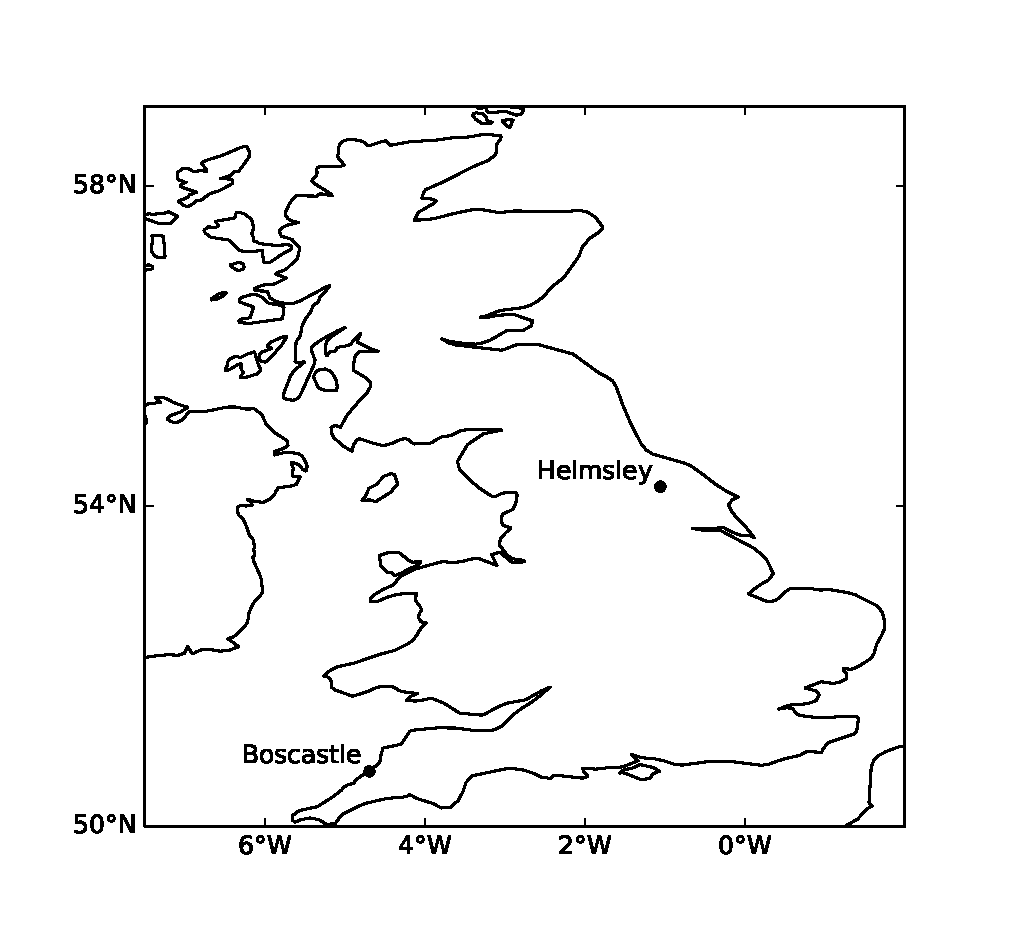
\includegraphics[width=11cm]{chp_events_figures_scripts/figure_location_map.eps}
\caption{Location of the two case study catchments in Britain, marked by the main settlement within each catchment.}
\label{fig_location_map}
\end{figure}

\linespread{1.5}
\begin{table}
\resizebox{\textwidth}{!}
{%
\begin{tabular}{l c c} \hline

Catchment Name 			& \textbf{Ryedale} &  \textbf{Valency} \\ \hline
Main settlement        & Helmsley             & Boscastle \\
Catchment Area   			& 270km$^2$ 				& 18km$^2$ \\ 
Catchment Type         & Upland, Moor/Peaty & Upland, Pasture \\ 
Storm Date	 		            & 2005-06-19 	& 2004-08-16 \\ 
Peak Rainfall	 (mm hr \(^{-1}\))  & 125  & c.400 \\
%Peak Discharge	 	 & & \\ 
Meteorological Setting	 	& Split-front, convective system & Quasi-stationary convective system \\ 
3hr Rainfall Return Period 	 & 330yr \citep{wass2008investigation}	& 1300yr \citep{burt2005cloudburst} \\ \hline
\end{tabular}
}
\caption{Table showing key characteristics of each storm event.}
\label{table_met_setting}
\end{table}

\subsection{Boscastle, Cornwall storm 2004}
The Boscastle storm took place on 16 August 2004. The storm led to flooding within the River Valency catchment and the village of Boscastle. In the preceding months March--June, the south-west area of Britain had been drier than usual, although during July the Valency catchment area experienced average rainfall conditions \citep{golding2005boscastle}. The estimated soil moisture deficit\footnote{The amount of water needed to bring the soil back to field capacity, i.e. a state where the soil is holding the maximum amount of water possible against gravity. \citep{beven2011rainfall}} in the area, which had previously been lower than average due to the dry antecedent conditions in March--June, decreased during 1--16 August, due to a return to average rainfall conditions in that month. The soil moisture deficit during this period was estimated to have decreased from approximately 80--220mm to 40--180mm \citep{golding2005boscastle}.

On the day of the storm, rainfall accumulations of up to 184mm from the Lesnewth tipping bucket raingauge \citep{golding2005boscastle} were recorded in the upper Valency catchment resulted from prolonged rainfall between 1200--1600 UTC. Rainfall rates were thought to have reached almost 400 mm hr\(^{-1}\) \citep{golding2005boscastle}, after correcting for under-reporting from rain gauges in the vicinity of the catchment \citep{burt2005cloudburst}. The rainfall accumulations from the 1km gridded composite radar product in the Valency catchment are shown in Figure \ref{fig_boscastle_rain_totals}. Note that the highest rainfall accumulations from the radar data shown in Figure \ref{fig_boscastle_rain_totals} are 115mm, lower than the raingauge totals reported in \citet{golding2005boscastle}, likely due to under reporting by precipitation radar. 

%The meteorological conditions that enabled such prolonged heavy rainfall were a combination of large-scale synoptic conditions moving in from the Atlantic, with moist lower atmospheric layers readily forming convective cloud. Repeated initiation of convection along the north Cornish coast lead to what appeared to be relative stationary convective cells over the Valency catchment. Later authors refer to this type of convective storm as a `Boscastle-type' or quasi-stationary convective storm \citep{warren2014boscastle}.

\begin{figure}[htb]
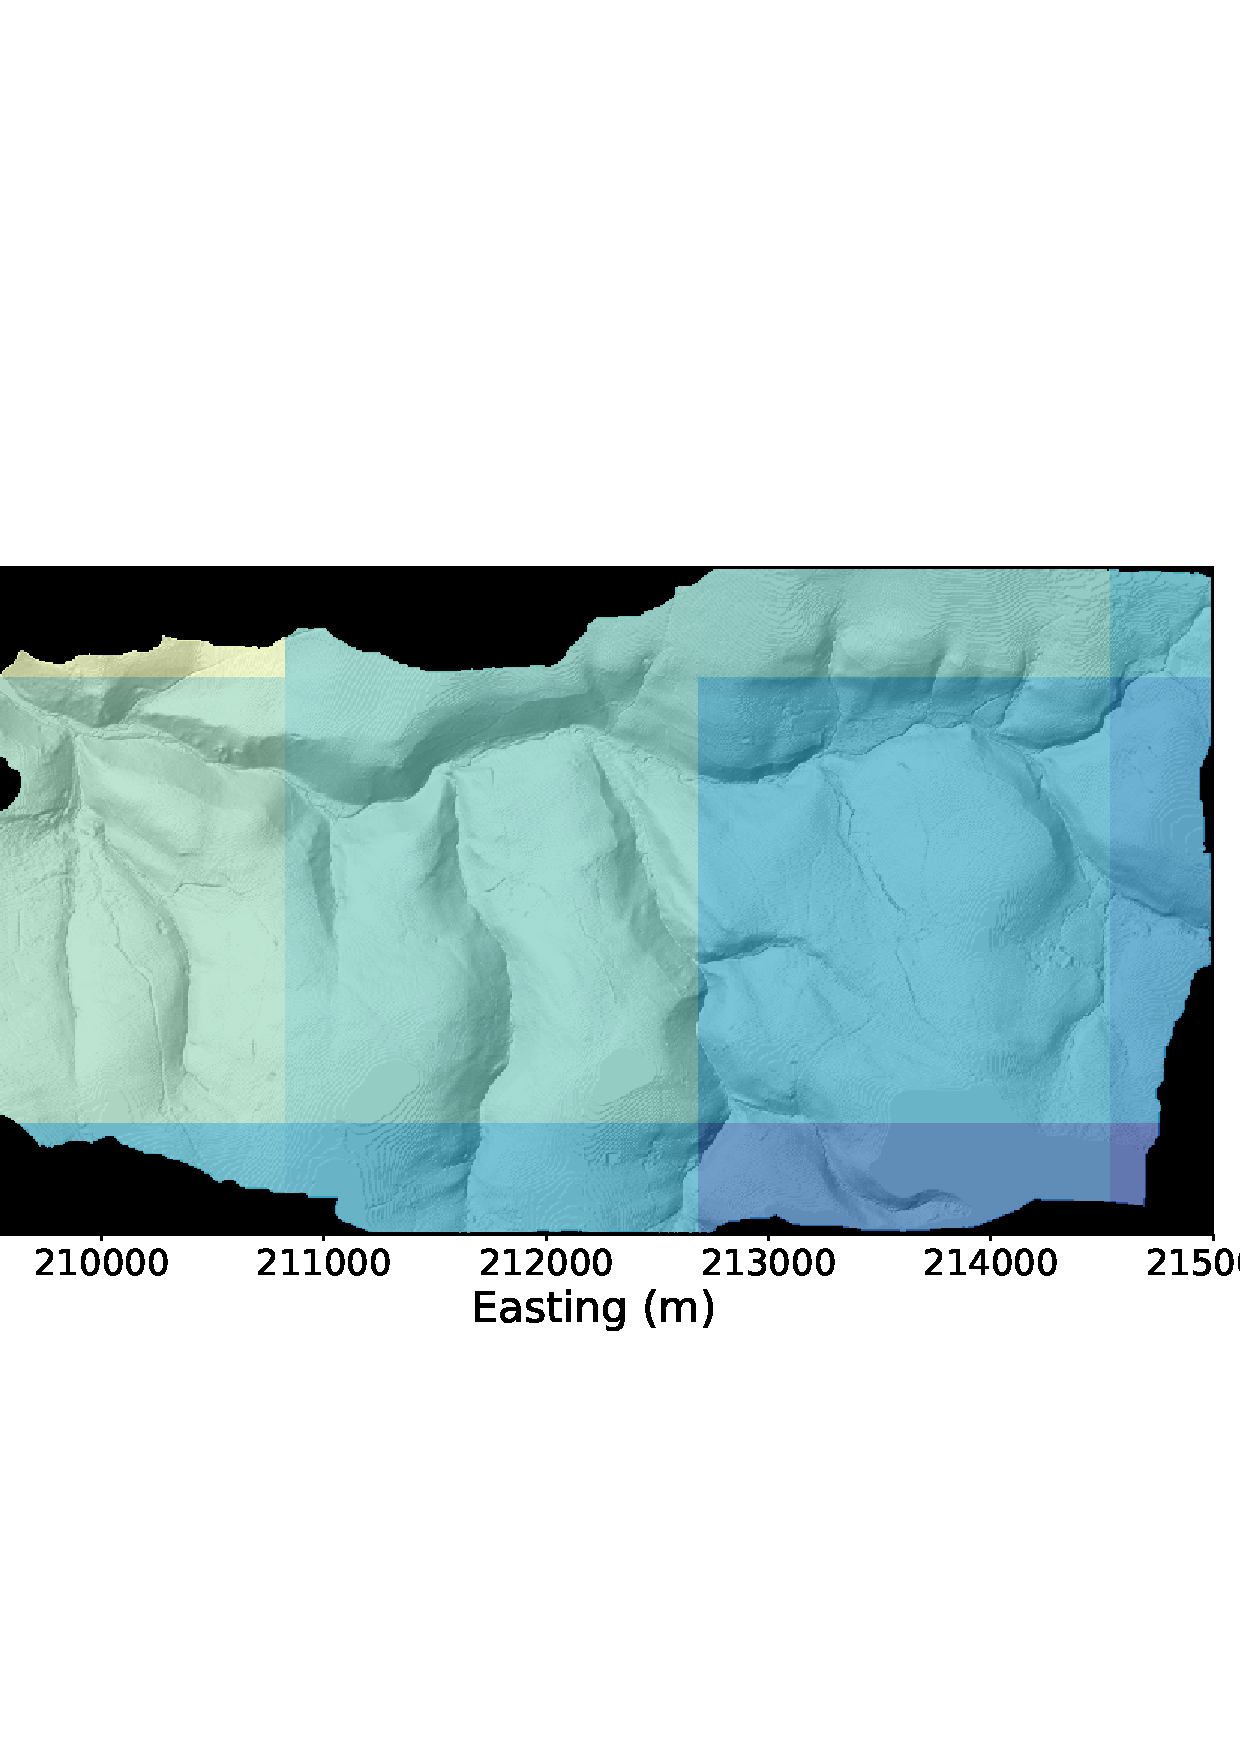
\includegraphics[width=15cm]{chp_events_figures_scripts/figure_boscastle_total_rainfall.png}
\caption{Total accumulated radar rainfall (24 hours) over the Valency (Boscastle) catchment during the 16th August 2004.}
\label{fig_boscastle_rain_totals}
\end{figure}


\subsection{Ryedale, North York Moors storm 2005}
The Ryedale storm occurred on 19 June 2005. Intense rainfall throughout the afternoon led to total accumulated rainfall amounts of up to 89mm in Ryedale between 1400--1800 UTC measured by the Helmsley raingauge. Peak instantaneous rainfall rates were estimated to have been around 32.5mm hr\(^-1\) \citep{sibley2009analysis} to 59.4 mm hr\(^{-1}\) \citep{hopkins2012knowledge}, though one report states they reached as high as 125 mm hr\(^{-1}\) \citep{cinderey2005north}. Figure \ref{fig_ryedale_rain_totals} shows the total accumulate rainfall radar totals from the 1km composite radar product. Most areas of the catchment received total rainfall accumulations similar to the reported raingauge figure (89mm), though up to 131mm is reported in one grid square in the south of the catchment area.

Antecedent conditions before the Ryedale storm of 2005 were dry over a prolonged period over much of the region \citep{sibley2009analysis}, leading to cracking of the surface peat in the higher elevations of the catchment. Soil moisture deficit was estimated to be around 60mm in the catchment, higher than usual due to the drier conditions in the preceding months \citep{wass2008investigation}. With a high soil moisture deficit, thinner soils in the upper reaches of the catchment would have been dry before the intense rainfall.

%The meteorological conditions leading to such heavy rainfall was a combination of a cold, upper-level air mass advecting over a warm moist boundary layer, leading to unstable conditions that enabled a convective thunderstorm to develop in the late afternoon. The conditions let to a particularly high amount of precipitable water present in the atmosphere which was subsequently washed out into the landscape during intense rainfall. 

\begin{figure}[htb]
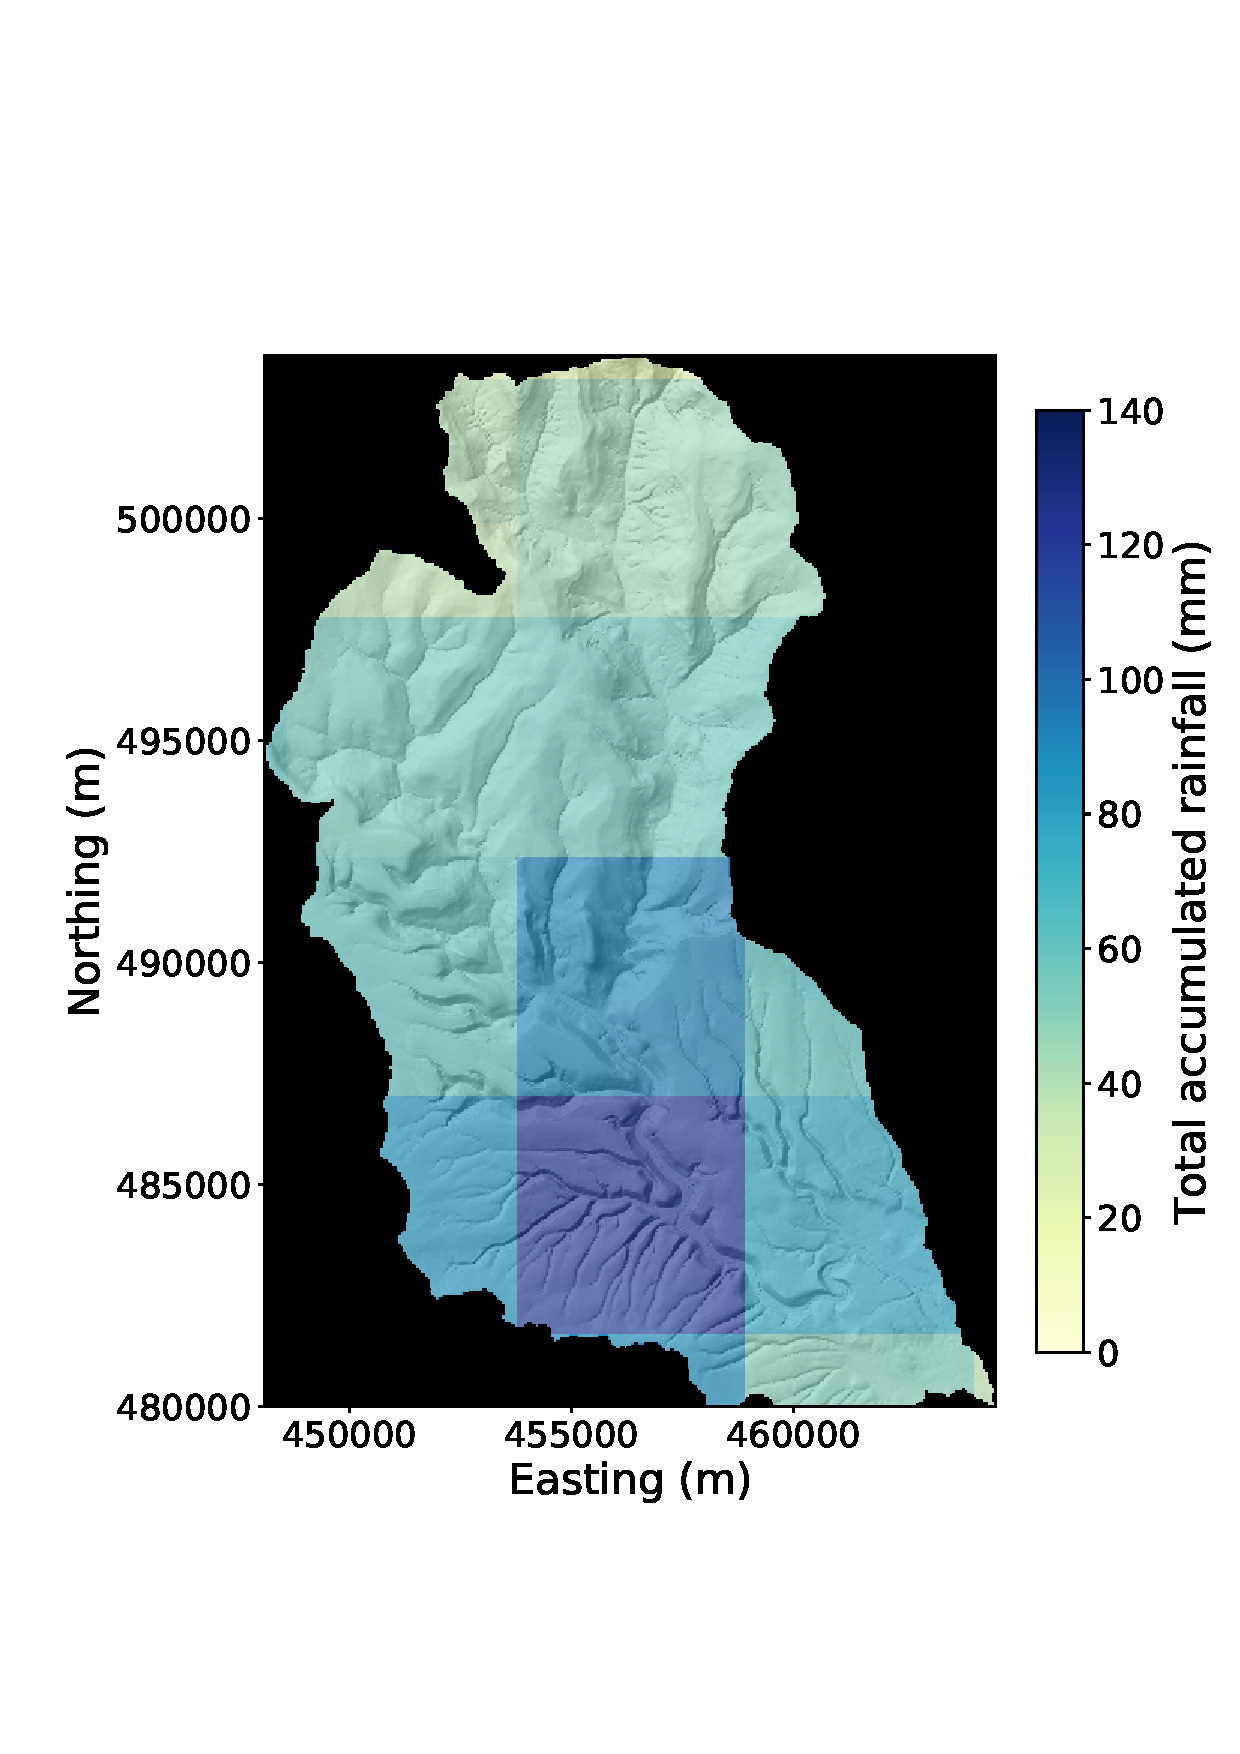
\includegraphics[width=13cm]{chp_events_figures_scripts/figure_ryedale_total_rainfall.png}
\caption{Total accumulated radar rainfall (24 hours) over the Ryedale catchment during the 19th June 2005.}
\label{fig_ryedale_rain_totals}
\end{figure}

\section{Flooding and geomorphic change}

\subsection{Boscastle, Cornwall, 2004}
Flooding was extensive in the area surrounding Boscastle village, with flood levels rapidly exceeding bankfull and flooding several properties to depths of several metres. Water levels in the Valency river and its tributaries began to rise in the early afternoon from approximately 1200 UTC onwards, reaching bankfull around 1430 UTC and peaking at around 1600 UTC, by which point over 70 properties had been flooded, with several destroyed due to the force of the water \citep{wallingford2005flooding}.

The routing of flood waters in the Boscastle flood was complicated due to the role of large debris blockages (`trash barriers') in the river channels. In particular, a large debris blockage formed under the main bridge in the village crossing the Valency, which caused a significant backup of water behind the bridge, and re-routing of water through alternate pathways within the village. A reconstruction of the flood based on eyewitness accounts and water mark levels consequently resulted in different reports of the peak water level in the village depending on where the observations were made \citep{wallingford2005flooding}. 

The geomorphological impacts of the flood event were well documented in the aftermath of the event \citep{wallingford2005flooding}. The Valency river channel and many of its tributaries experienced channel avulsion\footnote{Movement of the original channel to a new position within the flood plain.} in places, as well as significant downcutting in the upper tributary channels of the catchment. In a number of places the channel avulsion was substantial enough to straighten the channel and increase the local gradient of the river, potentially increasing flow velocities and shear stresses acting on the channel bed. There were large amounts of sediment observed in the river flow at the time, ranging in size from fine silts to boulders. There were some areas of sediment deposition observed along the river channel banks and floodplain, and a sizeable area of sediment deposition in Boscastle harbour. However, most stretches of the main river channel and its tributaries showed net erosion in the form of channel widening (up to 3--4 metres) and deepening (of up to 2 metres) \citep{wallingford2005flooding}.

\subsection{Ryedale, North Yorkshire, 2005}
Flooding was widespread in the Ryedale catchment, with river levels reaching up to 3.5m at Hawnby, a smaller settlement upstream of Helmsley. At the peak of the flood, the Hawby gauging station building was completely submerged\citep{wass2008investigation}. In Helmsley, the largest settlement, further downstream, similar river level rises of up to 2m were reported at the peak of the flood in the evening and into the night. 

Geomorphologically, the Ryedale catchment saw relatively rapid change considering the short duration of the storm and subsequent flood on 19 June. In the aftermath of the flood, up to 2--3 metres of channel downcutting and erosion were reported to have take place in the upper reaches of the tributaries of the catchment \citep{hopkins2012knowledge,wass2008investigation} as well as significant amounts of sediment and debris deposition in the lower reaches of the catchment around Helmsley \citep{hopkins2012knowledge}. The storm triggered many landslides on hillslopes within the catchment, including 105 reported shallow landslides in the catchment, as well as two large peat slides in moorland areas covering up to 3.7 ha of mass movement in areal extent \citep{galiatsatos2007assessment,wass2008investigation}. Dry antecedent conditions in the area are believed to have been a main cause of landsliding in the area by weakening the peat moorland within the catchment \citep{sibley2009analysis}. Dry conditions preceeding summer storms can cause shrinkage and cracking in peatlands, leading to greater risk of erosion in heavy downpours \citep{warburton2004hydrological}. 
The economic damage was also substantial for a sparsely populated area. Three bridges were destroyed at a cost of £2.9 million, as well as flooding of 121 properties \citep{wass2008investigation}. Economic loss included agricultural damage such as loss of land and livestock \citep{sibley2009analysis}. Many residents were displaced for months during repair and were reported to have suffered illness and psychological trauma from the event \citep{hopkins2012knowledge}.



\section{Experiment design}
\label{section_experiment_design}

Using the two flash flood events described previously as case studies, an ensemble of simulations was designed to address the questions laid out in Chapter \ref{chapter_intro} and summarised in the following hypotheses:

\begin{enumerate}

\item \label{itm:flood} \textbf{Flood inundation modelling is sensitive to the spatial detail of precipitation inputs.}
  \begin{enumerate} 
  \item \label{itm:hydro} Catchment hydrology is sensitive to the spatial distribution of rainfall inputs over the catchment area. Resolving the spatial details of a precipitation event, such as during a flash flood, allows the timing and magnitude of flood inundation to be better predicted.
  \item Geomorphological change of the river channel and flood plain during a flash flood is substantial enough to alter the patterns of flood inundation. In a model that can account for erosional change during flooding, nuances in flood inundation can be better predicted.
  \end{enumerate}

\item \label{itm:geomorph} \textbf{Erosional processes in river catchments are sensitive to the spatial distribution of rainfall inputs.}
  \begin{enumerate}
  \item Erosion and sediment transport processes are sensitive to thresholds determining erosion initiation and sediment entrainment. If item (\ref{itm:hydro})  holds true, then fluvial erosional processes should exhibit sensitivity to the spatial distribution of rainfall inputs of rainfall as well.
  \item The parameterisation of erosional processes in the model also determines the spatial pattern of erosion and deposition, but does spatial variation in rainfall inputs exert a greater control than the choice of erosion law?
  \end{enumerate}
  
\end{enumerate} 

To test the above hypotheses, simulations of the two case studies were repeated, varying the following conditions:

\begin{itemize}
\item Rainfall spatial resolution: 1km-gridded/uniform
\item Erosion law: transport-limited/detachment-limited
\end{itemize}

The simulations were parameterised with different erosion law schemes and different rainfall input resolutions to assess which factor exerted the greatest control over flood inundation and sediment transport within the catchment. The same set of experiments was carried out for both the Boscastle and Ryedale events, giving a total of 6 different simulations for each catchment outlined in Table \ref{table_ensemble_experiments} -- a total of 12 simulations.


\begin{table}
\begin{tabular}{lll}
\\
\textbf{Experiment name}   & \textbf{Rainfall input} & \textbf{Erosion law}  \\
\hline
UNIFORM\_HYDRO  &  Spatially-averaged  Radar  & (no erosion) \\
UNIFORM\_DLIM      &  Spatially-averaged  Radar & Detachment-limited \\
UNIFORM\_TLIM       &  Spatially-averaged  Radar & Transport-limited \\

GRIDDED\_HYDRO  &  1km Radar Gridded  & (no erosion) \\
GRIDDED\_DLIM      &  1km Radar Gridded  & Detachment-limited \\
GRIDDED\_TLIM       &  1km Radar Gridded   & Transport-limited \\
\hline \\ 
\end{tabular} 
\caption{Outline of the simulations carried out for both the Ryedale and Boscastle case studies.}
\label{table_ensemble_experiments}
\end{table}

\

\subsection{Model initialisation and configuration}
The numerical landscape evolution model, HAIL-CAESAR was used for all simulations. The equations describing the water routing, sediment erosion and transport laws are described fully in Chapter \ref{chapter_HAIL-CAESAR}.

Two erosion laws are used in the set of simulations with erosional processes `switched-on' in the model: a transport-limited law and a detachment-limited law. The transport-limited law represents erosion taking place under flowing water, which is limited by the capacity of the water to move away sediment. It assumes a constant supply of sediment is available, and that \textit{transportation} is the effective limiting factor on how much erosion takes place during water flow over hillslopes and in rivers. The transport-limited law in HAIL-CAESAR is based on the \citet{wilcock2003surface} sediment transport law, which accommodates multiple grain sizes across the sand to gravel particle size range. The equations describing the Wilcock and Crowe model are referred to in Section \ref{trans_model}.

The second type of erosion law used in the simulations is a bedrock incision law based on detachment-limited erosion. A detachment-limited law assumes that erosion is limited by the amount of material that can be \textit{detached} from the bedrock layer, based upon a critical shear stress exerted by water flow being exceeded to detach sediment material. The detachment-limited law is based on the same law used in the CHILD landscape evolution model (Chapter \ref{chapter_landscape_evol}) and the equations describing it are given in Section \ref{bedrock_model}.

The two erosional parameterisations used in these simulations represent two end-members of a spectrum of potential erosion laws that could be used. Upland catchments in the UK, and in these catchments in particular, tend to be a mixture of thin sediment layers and partially exposed bedrock. It was felt that limiting the number of erosion laws used to two end-members would constrain some of the uncertainty in selecting a sediment transport law appropriate for these types of catchment, similar to a landscape evolution modelling approach used by \citet{Attal2008}.
%
%HAIL-CAESAR is a hydrodynamic landscape evolution model that uses a TOPMODEL-based hydrological rainfall-runoff model to generate surface runoff in a river catchment, which is then routed through the landscape according to an adaptation of the LISFLOOD-FP shallow water routing algorithms \citep{bates2010simple}. Fluvial erosion and sediment transport is then derived using the velocities and depths of the calculated surface water within the catchment.

\subsubsection{Input data}
Rainfall input data is taken from the Met Office NIMROD radar rainfall 1km composite dataset \citep{metoffice2003nimrod}. The same 1km rainfall radar product is used to derive the rainfall inputs for the spatially uniform rainfall simulations, by averaging out the gridded rainfall data over the input points of the catchment, thus preserving the total amount of rainfall input in each simulation, and only varying its spatial distribution for the relevant gridded rainfall input simulations.

Topographic data used to initialise the terrain surface for the Boscastle simulation is derived from the Environment Agency (England) 2m LiDAR product. The Boscastle data is resampled to 5m grid spacing to reduce the total number of grid cells and the  computational demands of running a complex hydrodynamic model. Environment Agency LiDAR was not available for the whole Ryedale catchment at the time of the simulation, so the Ryedale terrain is initialised using Ordnance Survey `Terrain 50' data, interpolated to 5m grid spacing to enable like-for-like comparison with the Boscastle terrain grid spacing. Resampling the initial topographic data sources to the same terrain grid spacing of 5m for both sets of simulations is done to minimise the potential effects that variation in grid spacing has on model output and subsequent topographic analysis \citep[e.g][]{chang1991effect,schoorl2000three,haile2005effects,zhang2008effects}

\subsubsection{Simulation duration}

The simulations are set to begin 24 hours before the day of each storm event. The model is allowed to run for a further 24 hours after the event, giving a total simulation time of 72 hours. The timing of the simulations is given in Table \ref{table_start_time_hydrog_sims}.

\begin{table}[htbp]
\begin{tabular}{l c  c}
\textbf{Event}  &   \textbf{Start time} &  \textbf{End time} \\
\hline 
Boscastle          &  2004-08-15 00:00  &  2004-08-17 23:59 \\
Ryedale             &  2005-06-18 00:00  &  2005-06-20 23:59 \\
\hline

\end{tabular}
\caption{Start and end times (UTC) for each 72 hour simulation. The major rainfall event occurs during the second day in each simulation.}
\label{table_start_time_hydrog_sims}
\end{table}

\subsubsection{Rainfall spatial resolution}
In order to assess the sensitivity of hydrogeomorphic processes to the spatial details of precipitation, rainfall spatial inputs were alternated in each simulation between a spatially uniform rainfall input and a 1km gridded rainfall input. Both the spatially uniform and gridded inputs were based on the same original rainfall source data -- the UK Met Office Nimrod 1km-composite radar data product \citep{metoffice2003nimrod}. The uniform rainfall input data were created from averaging out the gridded data in spcae over the model domain. The temporal resolution of the five minute interval data was preserved, giving a time series of spatially averaged rainfall rates for the duration of the each simulation. To reduce the range of variables within the set of ensemble simulations, only the spatial resolution of rainfall was assessed in this study -- other studies had already investigated the effects of the \textit{temporal} resolution of rainfall data on discharge and erosion rates \citep{nicotina2008impact,Coulthard2013,coulthard2016sensitivity}. In all experiments, the temporal resolution of rainfall data was maintained at five minute intervals. To summarise, the two types of rainfall spatial input used were: 

\begin{itemize}
\item Uniform or `lumped' precipitation: Radar-derived rainfall rates across the catchment are spatially-averaged to produce a catchment-wide rainfall rate. In other words, every grid cell in the model domain receives the same rainfall rate at each five minute rainfall data timestep.
\item Gridded rainfall input. The rainfall rate is input from a overlying gridded mesh of raincells, at the same grid spacing as the rainfall radar product (1km).
\end{itemize}

\subsubsection{Erosion-enabled simulations}
A variety of erosion laws exist describing how landscapes erode from fluvial erosion. The choice of erosion law for a given catchment depends on a variety of factors, such as the characteristic substrate material in the catchment -- is it predominantly loose sediment or cohesive, solid bedrock? In reality, many upland landscapes in the UK are often a mixture of these two extremes, incorporating a thin layer of loose sediment on top of solid bedrock. Streams in such landscapes may be termed mixed-channel systems \citep{howard1998long}, and many variants on the fluvial incision laws incorporating the role of sediments have been proposed \citep{Lague2005,sklar2006role}. Catchments also often exhibit a transition from rockier upland headwaters, to more thickly soil-mantled floodplains. In order to address the sensitivity to the choice of erosion model for each event simulation (Chapter \ref{chapter_landscape_evol}), two erosion model end-members are used, with each one representing a different conceptual model of fluvial erosion and sediment transport. These include: i) a purely sediment transport-limited model \citep{wilcock2003surface}, ii) a detachment-limited bedrock erosion model \citep{howard1983channel,stock1999geologic,whipple1999dynamics}. The equations describing the transport-limited and detachment-limited models used in the model are discussed in detail in Chapter \ref{chapter_HAIL-CAESAR}. Further erosion laws were considered, such as a hybrid transport- and detachment-limited erosion model, but it was deemed beyond the scope of this study, which is primarily to investigate the role of rainfall heterogeneity, rather than the wide range of erosion and sediment transport models. In keeping with the primary aim of the study, it was opted to use two simple variants of sediment erosion laws to keep the range of model simulations parsimonious. 

\subsubsection{Flood inundation only simulations}
A set of control simulations (suffixed \textit{HYDRO}, for example in Table \ref{table_ensemble_experiments}) incorporating only rainfall-runoff and surface water routing (with no erosion taking place) were also carried out for comparison against the two erosion end-member simulations. The analysis from these experiments is used to investigate the sensitivity of flood-inundation prediction to geomorphic change during floods, and the results and discussion are presented in Chapter \ref{chapter_flood_model_sensitivity}.

%\paragraph*{Hybrid model}
%The hybrid model assumes a limited-depth sediment layer, overlying a bedrock layer. Figure \ref{hybrid_model} shows a typical cross section through a typical valley in the hybrid model set-up. In the initial model state (before the spin-up period), a channel is 'burnt-in' to the sediment-layer. Whenever bedrock becomes exposed during the hybrid simulation, the simple detachment-limited erosion law is applied. Material removed from the bedrock layer is then apportioned between the various sediment fractions. At all other times, the sediment transport law applies to the sediment layer. 



%\subsubsection{Model spin-up}
%
%The HAIL-CAESAR model (Valters ?\& Coulthard?, 2016/7) initialises the model domain with a uniform distribution of sediment grain sizes across the catchment. This is physically unrealistic, so the model domain is `spun-up' for a simulated time of 1000 days using typical rainfall data for each catchment. This ensures a heterogeneous distribution of sediment throughout the catchment prior to the detailed storm simulations. 

\section{Summary}

Using case studies from two flash flood events in the UK that took place in recent decades, a series of simulations was designed to investigate the effects of rainfall spatial resolution on flood inundation modelling, and sediment erosion and transport. The simulations are designed to answer the questions laid out in Chapter \ref{chapter_intro} and the hypotheses summarised in Section \ref{section_experiment_design}. 

The results and analyses from the simulations are discussed in the subsequent chapters. Chapter \ref{chapter_flood_model_sensitivity} analyses and discusses the effects that rainfall spatial resolution has on flood inundation prediction in the HAIL-CAESAR numerical model, and also looks at the effects that geomorphic change during a flood has on flood dynamics. This addresses Question \ref{itm:flood} laid out in Section \ref{section_experiment_design} above. 

Chapter \ref{chapter_hydrogeomorph} analyses the results of the simulations focusing on sediment erosion and transport, discussing whether the spatial patterns of rainfall control the distribution of erosion and deposition in a catchment. The implications for longer-term landscape evolution modelling are also discussed. Chapter \ref{chapter_hydrogeomorph} addresses Question \ref{itm:geomorph} laid out in Section \ref{section_experiment_design} above. Conclusions and links between rainfall inputs, hydrological, and geomorphological processes are discussed in Chapter \ref{chapter_conclusion}.


%=-=-=-=-=-=-=-=-=-=
% RESULTS AND INTERPRETATION
%=-=-=-=-=-=-=-=-=-=

% Chapter 6 describes a case study test of using the model with hi res rainfall
% radar data
\chapter{Sensitivity of a flood-inundation model to rainfall distribution and erosional parameterisation}
\label{chapter_flood_model_sensitivity}
\chaptermark{Flood inundation model sensitivity}
%\begin{refsection}


%\begin{abstract}
%Landscapes evolve and take their shape from the cumulative effect of `geomorphically effective' events. In temperate climates, these are rainfall-driven events of sufficient magnitude to trigger threshold-dependent erosional processes. This chapter investigates the sensitivity of two end-member erosional models to the spatial resolution of rainfall input to a catchment using three historic severe rainfall events in Northern England and Cornwall.
%
%It is demonstrated that the erosional model chosen exerts first-order control of the total amount of landscape change and sediment flux. However, both end member models show sensitivity to the spatial resolution of rainfall input data during individual, formative rainfall events. 
%
%\end{abstract}
\section{Introduction}

Flooding from intense rainfall poses great risk to communities living in proximity to rivers and has the potential to cause loss of life and substantial economic damage in affected areas \citep{pitt2008pitt}. Reliable prediction and advanced warning of flooding requires an understanding of the hydrological processes that operate within a river catchment, in order that operational flood forecasting models may be better parameterised and developed to mitigate against the impact of future events. The interaction of environmental processes within the river catchment system is sensitive to a number of external and internal forcings, including but not limited to precipitation input \citep{nicotina2008impact}, catchment vegetation cover \citep{darby1999effect,andreassian2004waters,bradshaw2007global}, preconditioning of the catchment water table and soil moisture store by antecedent conditions \citep{berthet2009crucial}, urbanisation \citep{hollis1975effect}, debris mobilisation and blockage in river channels \citep{gippel1995environmental,jeffries2003influence}, as well as channel morphological change during flood events \citep{wong2015sensitivity}. 

%Spatial resolution
The question of whether spatial detail in rainfall inputs to a river catchment affects the hydrological response is unresolved, with a number of different studies putting forward seemingly conflicting conclusions. Early studies using deterministic modelling of river catchments and synthetic rainfall fields \citep{wilson1979influence} suggested that detailed space-time representations of rainfall were needed in distributed hydrological models. However, no allusion was made to the possible effects of varying catchment scales. In terms of predicting peak discharge in a catchment \citep{krajewski1991monte}, a small catchment (7.5km\(^2\)), was found to be sensitive to the temporal resolution of rainfall input data, but less so to the spatial distribution of rainfall inputs.  
The role of catchment size is likely to play a part in determining sensitivity to rainfall distribution, with several studies suggesting catchment size can dampen the effect of rainfall spatial variability \citep{segond2007simulation,nicotina2008impact}. The idea of catchment-size dependence has been developed further \citep{gabellani2007propagation}, suggesting that sensitivity to rainfall spatial heterogeneity depends on the characteristic size of the rainfall feature and the catchment size. Systematic investigation of the role of catchment size and morphology have suggested that is specifically the ratio between characteristic hillslope length of the catchment and the rainfall feature that determine sensitivity to spatial heterogeneity \citep{nicotina2008impact}. In cases where the rainfall feature is much greater in size than the typical hillslope length, the effects of rainfall heterogenity on runoff and hydrological response are muted. 

%Morphology change
Understanding how flood dynamics interact with channel and floodplain morphological change is of growing concern for flood modelling \citep{fewtrell2011geometric}. Morphological change during flood events has been shown to be a potential control in the extent of flooding during intense rainfall \citep{wong2015sensitivity}, particularly when river channels undergo geomorphically rapid change during repeated rainfall events of high magnitude \citep{slater2016extent}. Within the context of a single flood, bedload sediment may become highly mobile, and the forces acting on the boundaries of the river channel are sufficient to alter channel geometry in long profile, cross-section, and channel pattern \citep{wong2015sensitivity,kleinhans2013splitting}. As a counterargument, it has ben put forward that during large flood events the floodplain and river channel effectively act as one channel unit, dampening any effects brought about by changes to river channel morphology \citep{bates2005numerical}. The implications of sediment transport and erosion within river catchments has been highlighted as an important factor in flood inundation modelling \citep{lane2007interactions,lane2008reconceptualising,neuhold2009incorporating}, and should form part of an effective flood modelling strategy \citep{wong2015sensitivity} in catchments thought to be sensitive to morphological change during large floods.

% Bring two together.
Flood inundation prediction studies rarely consider both morphological change during flooding or spatial heterogeneity in rainfall inputs to the catchment. Given the reported importance of rainfall resolution on predicting increased sediment yields and channel incision over decades \citep{coulthard2016sensitivity}, can the same observation be made at the time scale of a single event, and does this in turn control the dynamics of a given flash flood event? Though there are differing conclusiions as to importance of rainfall heterogeneity and channel morphological change in flood inundation modelling, there is at least agreement that both have the potential to alter the outcome of flood prediction, under certain conditions. More investigation is needed into which of these uncertainties plays the greater role in determining flood inundation patterns during intense rainfall events and the analysis presented in this chapter attempts to address this by comparing flood inundation model predictions under different rainfall spatial resolution scenarios and erosion law parameterisations. 

%Climate impact etc.
%Growing consensus indicates that intense rainfall events are becoming more frequent in the UK \citep{kendon2014heavier}.

The following questions are explored through the use of numerical modelling experiments set out in Chapter \ref{chapter_events}, Table \ref{table_ensemble_experiments}

\begin{enumerate}
\item Are predicted flood inundation extents during a storm sensitive to the spatial resolution of rainfall inputs to the catchment?
\item Are fluvial erosion and sediment transport controls on predicted flood inundation extents during a single severe storm?
\item Does geomorphic change of the floodplain and channel during a storm event significant enough to affect flood inundation predictions?
\end{enumerate}

%%%%%%%%%%%%%%%%
%\section{Experiment Design \& Method}
%%%%%%%%%%%%%%%%

%\subsection{Rainfall-runoff and flow routing}
%From rainfall input, runoff is calculated using an adaptation of the Beven and Kirby (1979) TOPMODEL. Total surface and subsurface discharge is given by:
%
%\begin{equation}
%Q_{tot} = \frac{m}{T}\log \left( \frac{(r - j_t) + j_t \exp \left( \frac{rT}{m} \right) }{r} \right)
%\end{equation}
%
%where \(T\) is the time step in seconds, \(r\) is the rainfall rate, \(j_t\) is a function that describes soil moisture store, and \(m\) is a parameter that controls the rise and fall of this soil moisture store in \(j_t\). These adapted TOPMODEL equations are given fully in Coulthard (2002), equations (1) and (2).
%
%The amount of water partitioned between surface and subsurface flow is determined by a simple infiltration threshold, given by:
%
%\begin{equation}
%I_t = KS(Dx)^2
%\end{equation}
%
%where \(K\) is hydraulic conductivity, \(S\) is the slope, and \(Dx\) is the width of the grid cell or horizontal grid spacing. The infiltration threshold is subtracted from \(Q_{tot}\) to give the portion of water routed over the surface.
%
%Surface water and channel flow is an important driver in catchment scale erosional processes. The amount and velocity of water flow is a variable in both the sediment transport and bedrock erosion laws. The water flow equations are based on a simplified form of the shallow water flow equations, a simplification first derived by Bates (2010) and incorporated into the landscape evolution model by Coulthard et al (2013). The flow between cells is calculated by:
%
%\begin{equation}
%Q = \frac{q - g h_{flow} \Delta T \frac{\Delta (h+z) }{\Delta x}}{1 + g h_{flow} \Delta t n^2 |q| / h_{flow}^{10/3}} \Delta x
%\end{equation}
%
%where \(q\) is the water flux between cells from the previous iteration, \(g\) is acceleration due to gravity, \(h_{flow}\) is the maximum depth of flow between cells (m), \(t\) is time (s), \(h\) is depth of water, \(z\) is elevation, \(x\) is the grid well width, and \(n\) is Manning's roughness coefficient. The full implementation details are given in Coulthard (2013), and the derivation from the shallow water equations is given in Bates (2010).
%
%\subsection{Sediment transport}
%Transport of loose sediment within the model is governed by the \citet{Wilcock2003} sediment transport model. The Wilcock and Crowe model represents transport of mixed sand/gravel fractions based on the surface sediment composition. The rate of sediment transport, \(q_i\), is given as:
%
%\begin{equation}
%q_i = \frac{F_i {U_*}^3 {W_i}^*}{(s -1) g}
%\end{equation}
%
%where \(F_i\) is the fractional volume of sediment, for a given sediment fraction, \(i\), \(U^*\) is the shear velocity, \(s\) is the ratio of sediment to water density. \({W_i}^*\) is a function relating fractional transport rate to total transport rate (see \citet{Wilcock2003} for a full derivation of this equation). The usage of this sediment transport model is extrapolated here to account for finer particles such as silts \citep{Vandewiel2007}, as well as the sand-gravel mixture it was originally designed for.
%
%\subsection{Bedrock incision}
%\label{bedrock_model}
%A simple model of bedrock incision based on the excess shear stress model (Citations) is implemented in the numerical model. The rate of bedrock incision is determined by the amount of shear stress acting on the bedrock, above a threshold level of stress required to initiate substrate removal (e.g. \citet{Snyder2003}. When bedrock material is removed, it is distributed amongst the sediment fractions according to the fractional proportions set by the user. The rate of bedrock erosion according to the excess shear stress model is given by:
%
%\begin{equation}
%\varepsilon = k_e(\tau_b - \tau_c)^{P_b}
%\end{equation}
%
%where \(k_e\) is the bedrock erodibility coefficient, \(\tau_b\) is the basal shear stress on the channel bed, \(\tau_c\), is the critical shear stress threshold, \(P_b\) is the shear stress exponent. (Cite Howard or Whipple?)

%%%%%%%%%%%%%%%%%%%%%%%%%%%%%
%\subsection{Study area}
%%%%%%%%%%%%%%%%%%%%%%%%%%%%%%
%\subsubsection{Overview}

\section{Sensitivity analysis}
There are numerous user defined parameters in the HAIL-CAESAR model, and in landscape evolution models in general, that have a wide range of potential values. Parameter selection in environmental modelling comes with a degree of uncertainty, and resulting outputs from models can be highly sensitive to the user's choice of input parameters for a given simulation \citep{Pelletier2012}. Initial testing of the HAIL-CAESAR model, and studies using the CAESAR-Lisflood model that it is based upon show it is particularly sensitive to the TOPMODEL \textit{m} parameter, a parameter that controls the rise and fall of the soil moisture store, and hence how a river catchment responds to rainfall input \citep{beven1979physically}. 

To assess the sensitivity of the model to the choice of TOPMODEL-\textit{m} parameter, a series of simulations were carried out with a range of \textit{m} values for both test cases. Simulations of each flood event were carried out with the \textit{m} values shown in table \ref{table-m-sens}.

\begin{table}
\begin{tabular}{lc}
\textbf{Catchment} & \textbf{TOPMODEL \(m\) parameter} \\
\hline
Boscastle   &                                            \\
Ryedale     & 0.03, 0.04, 0.05, 0.06, 0.07, 0.08, 0.09, 0.1, 0.15, 0.2  \\
\hline
\\ 
\end{tabular}
\caption{TOPMODEL \(m\) parameter values used to run sensitivity simulations for each catchment.}
\label{table-m-sens}
\end{table}

%%%%%%%%%%%%%%%%%
\section{Results}
%%%%%%%%%%%%%%%%%

\subsection{TOPMODEL sensitivity}

The model exhibited a strong sensitivity to the choice of the TOPMODEL \( m\) parameter. In the results presented in figure \ref{fig_topmodel_m_ryedale} peak river discharge ranged from XX at an \(m\) value of 0.003 to XX with an \(m\) value of 0.008. The measured peak discharge reported for the 2005 storm at the Ness gauging station was 105 cumecs. In the sensitivity simulations, a value of \(m = 0.005\) produced a flood peak most closely matching the observed value, peaking at XX cumecs (Note the time as well.). 

There were differences between the hydrographs of the observed and simulated discharges in terms of peak discharge timing and recession limb shape. The observed hydrograph showed a sharp rise at around 50 hours after the start of the simulation period. Lower \(m\) values (m \textless 0.005) resulted in a prediction of the flood peak being too early compared to the observed timing, with values \textgreater \ 0.005 predicting the flood peak timing too late. Most of the simulations failed to capture the extended duration of peak discharge, which lasted approximately 5--6 hours, before receding back to low flow levels. The simulation with \(m = 0.006\) came closest to predicting this hydrograph shape, but failed to predict the magnitude of water discharge correctly, underestimating the peak flow by almost 50\%. 

For Ryedale simulations, it was decided to use an \(m\) value of 0.005, providing the closest possible match to the flood peak discharge, though not the true shape of the hydrograph and the receeding limb. As the catchment simulations include a representation of erosion and sediment transport processes, which are often threshold dependent, it was felt necessary to match the discharge peak more closely over choosing to match the hydrograph shape precisely.

\begin{figure}[t]
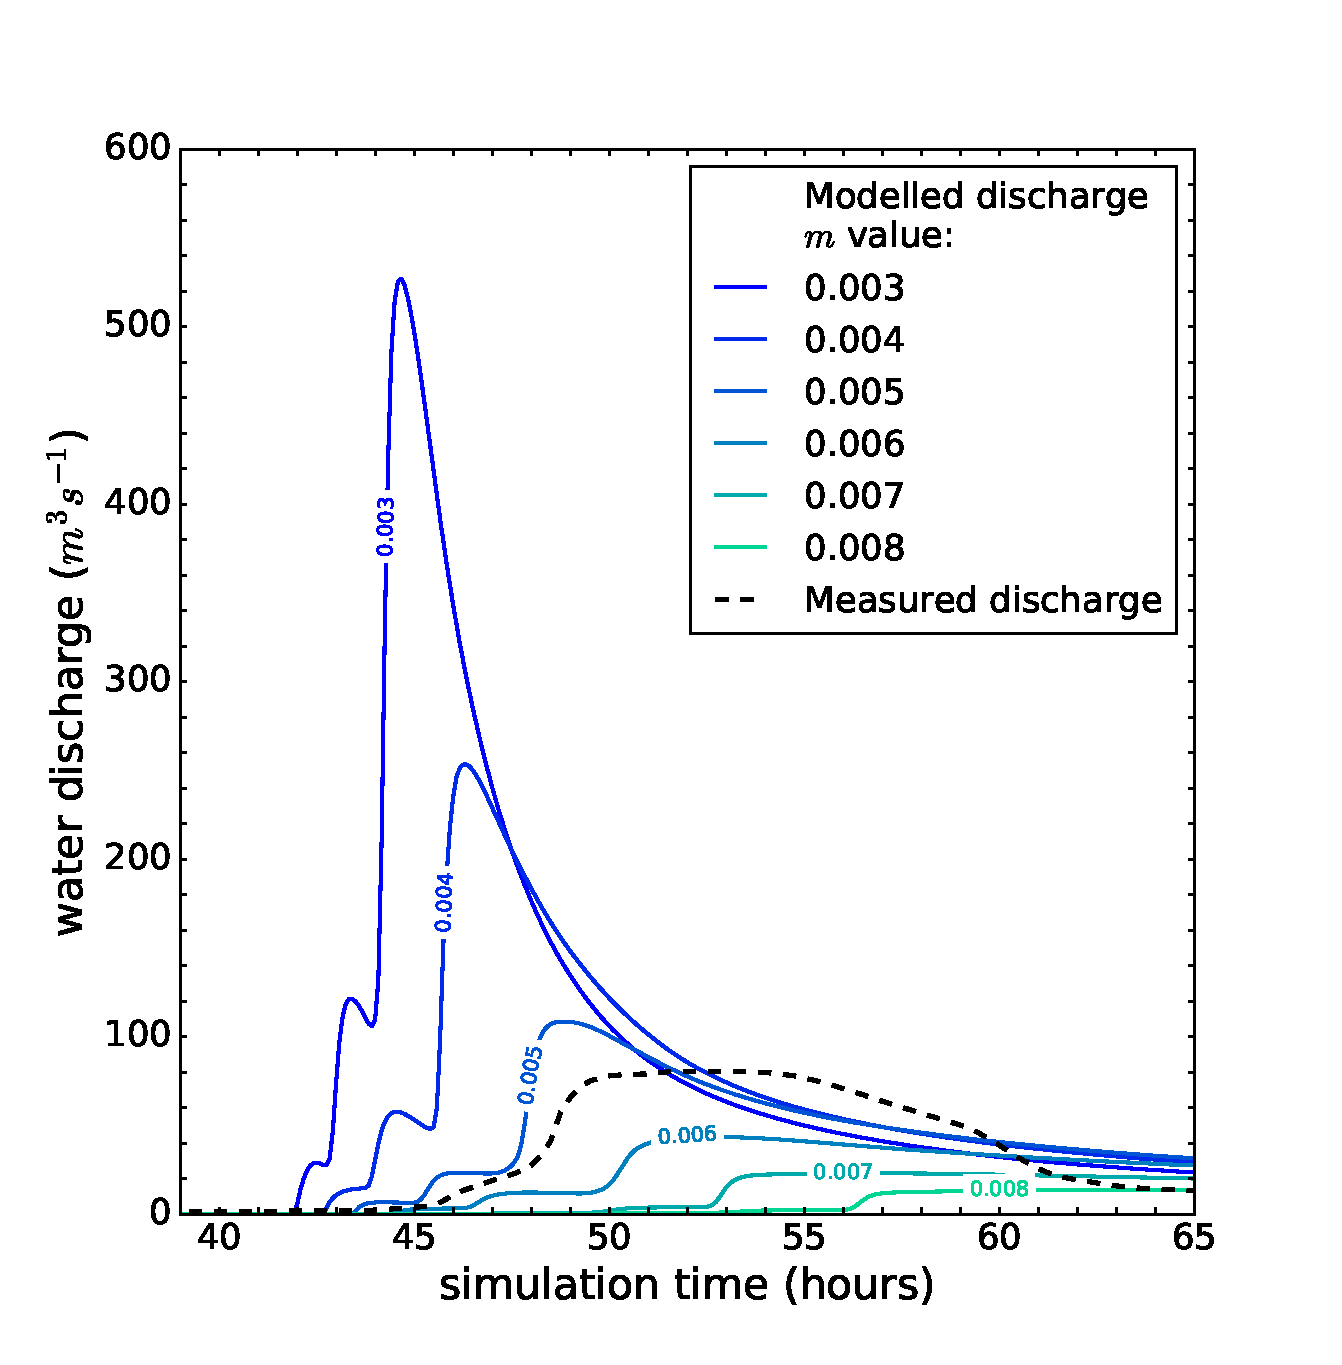
\includegraphics[width=11cm]{chp06_figures_scripts/figure_ryedale_M_sens.eps}
\caption{Discharge at Ryedale catchment outlet for varying values of the TOPMODEL \(m\) parameter. The measured discharge at the catchment gauging station is overlain in dashed line. The results from the simulations with \(m\) \textgreater \ 0.008 are omitted for clarity due to the low peak discharges they produced.}
\label{fig_topmodel_m_ryedale}
\end{figure}

\subsection{Catchment hydrology}

%Comparisons with the actual hydrographs from the gauged basins?

At the catchment scale, hydrological response was sensitive to both the rainfall resolution and the choice of erosional model. For both catchments, higher resolution rainfall input data resulted in a greater maximum river discharge. In the Ryedale experiments, simulations using the gridded rainfall input experienced a flashier hydrological response, reaching peak discharge several hours before the uniform rainfall input cases. This was not observed in any of the Boscastle simulations, with all simulations reaching peak discharge within 30 minutes of each other.

The choice of erosion model also influenced the hydrological response. When catchment erosion was modelled using a transport-limited case, peak discharges were higher in all cases, but the timing of hydrograph peaks remained similar for each case. The difference in peak discharges were minimal when comparing the detachment-limited cases to the hydrological-only models.

\begin{figure}[t]
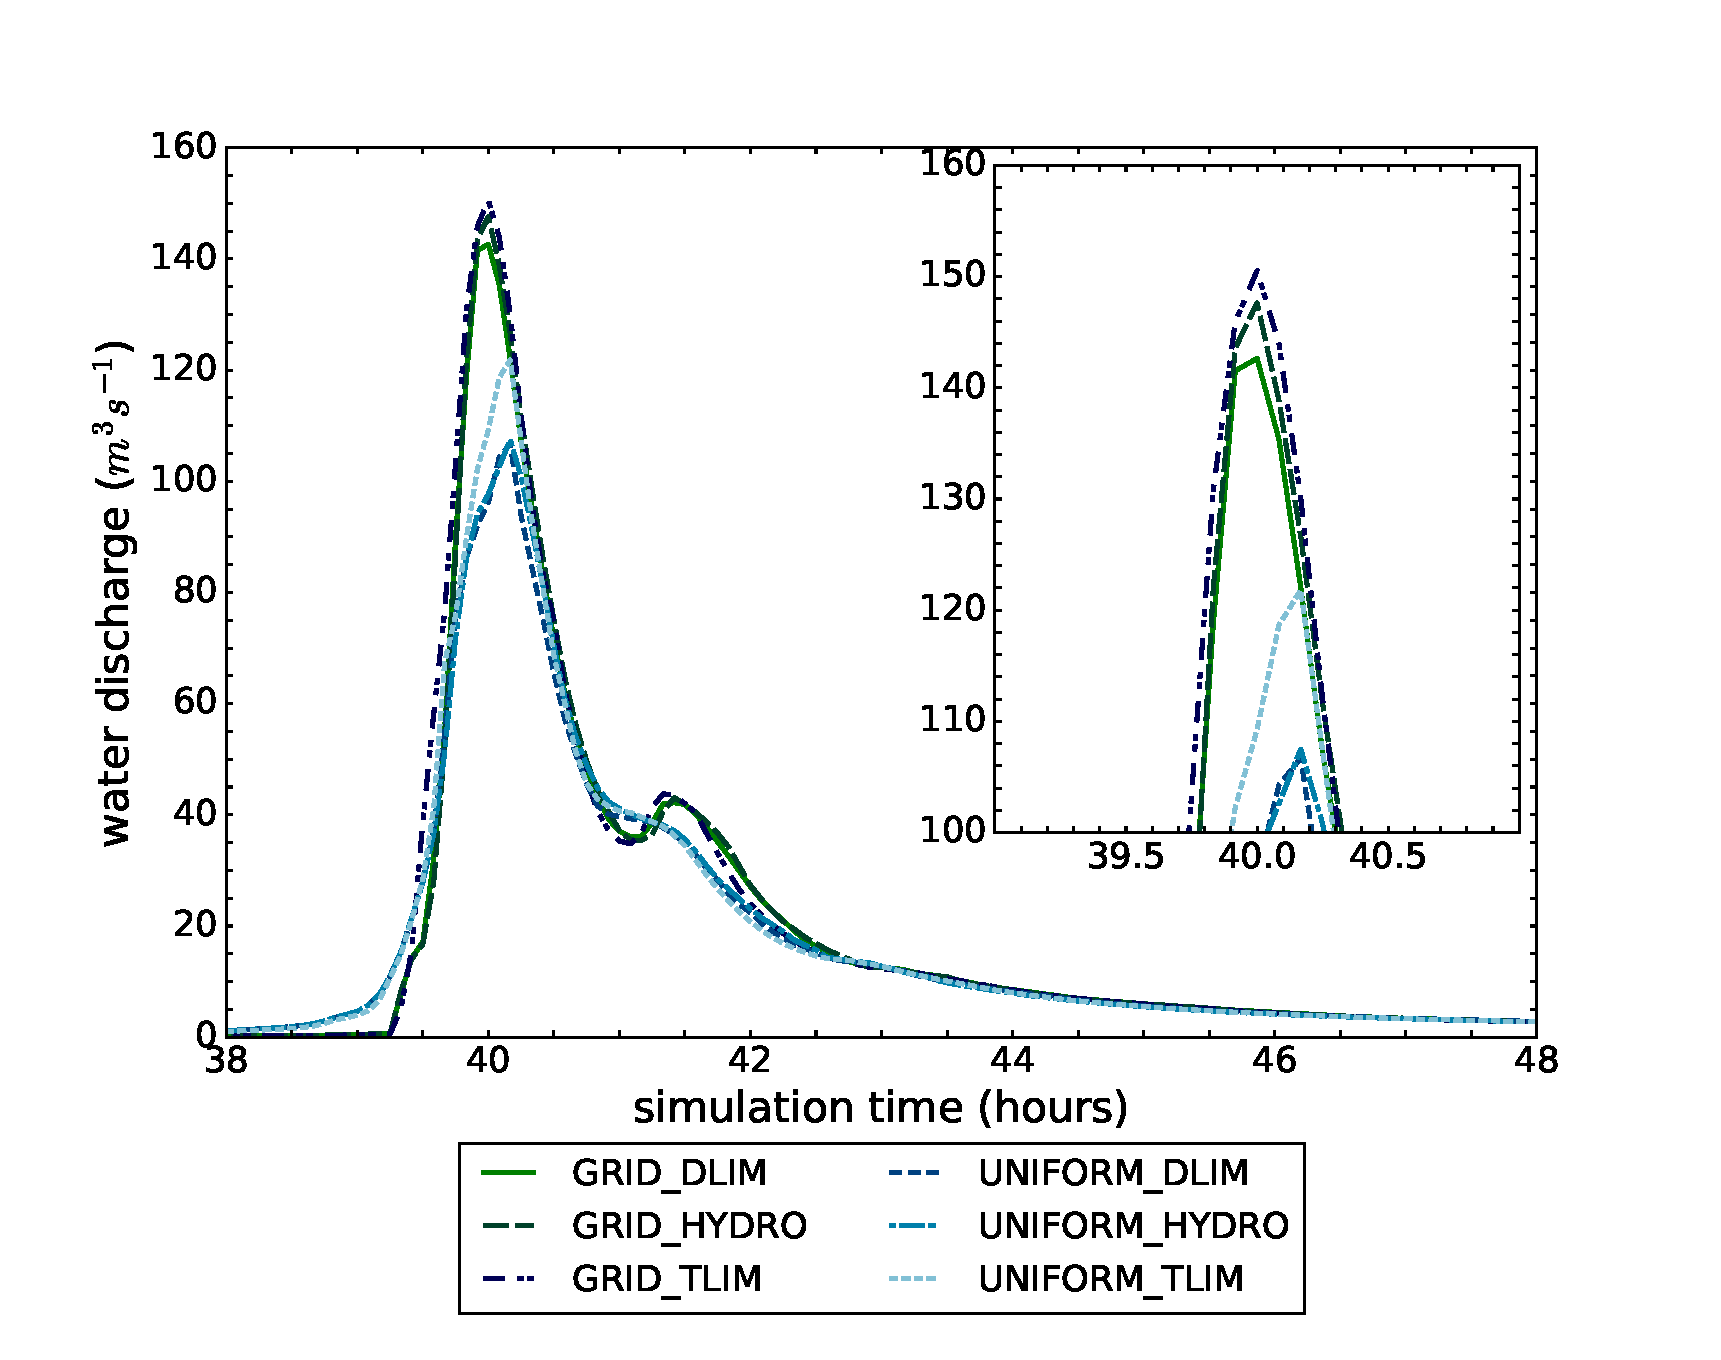
\includegraphics[width=14cm]{chp06_figures_scripts/figure_boscastle_hydrograph_ensemble.eps}
\caption{Boscastle hydrographs (discharge over time at catchment outlet) for each simulation of the 2004 Boscastle event listed in Table \ref{table_ensemble_experiments}. Inset shows detail of main flood peaks around hour 40 of the simulation.}
\label{fig_boscastle_hydrograph_ensemble}
\end{figure}

\begin{figure}[t]
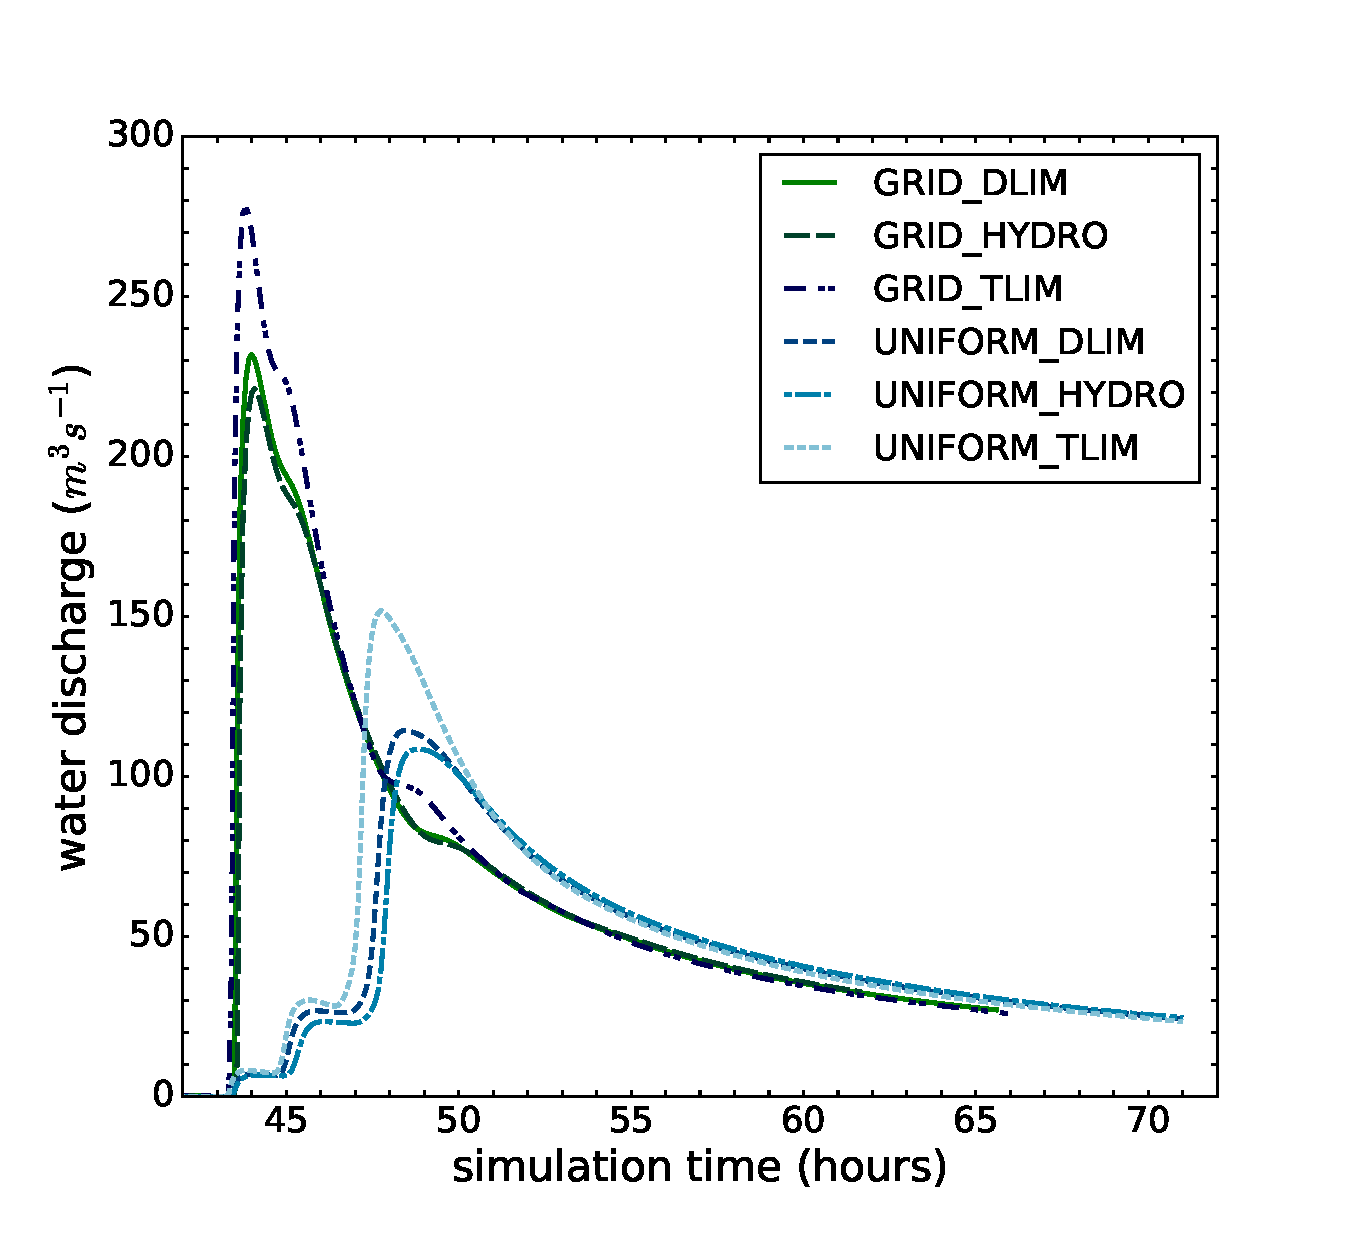
\includegraphics[width=14cm]{chp06_figures_scripts/figure_ryedale_hydrograph_ensemble.eps}
\caption{Ryedale hydrographs (discharge over time at catchment outlet) for each simulation of the 2005 Ryedale event listed in Table \ref{table_ensemble_experiments}.}
\label{fig_ryedale_hydrograph_ensemble}
\end{figure}



\subsection{Spatial variation in flood inundation}
\subsubsection{Boscastle}
The Boscastle catchment simulations showed minimal variation in flood inundation extent. Simulations with gridded rainfall input did not result in substantially different predictions of floodwater inundation compared to those with uniform rainfall input. Both sets of simulations reflected the general extent of reported flood water extents \citep{wallingford2005flooding}. Simulations that allowed erosion to take place (GRID\_TLIM and UNIFORM\_TLIM) showed a slight difference in the variation of floodwater depths in the floodplain area, particularly in the vicinity of Boscastle village, where Figure \ref{fig_boscastle_2dplan_flood_ensemble} is centred on. In hydrological-only simulations, the deepest water depths were predicted to occur in the confines of the river channel, whereas in erosion-enabled simulation, there appeared to be a `smoothing' effect of water depths between the channel and the adjacent floodplain, suggesting that the channel geometry had altered during the flood event either by infilling from sediment from upstream or collapse of the adjacent river banks. Engineer's reports of the Boscastle flood noted that the river channel in the Boscastle village area had indeed been inundated with debris during the storm, which had potentially contributed to the extent of the flooding within the village.

\subsubsection{Ryedale}
The Ryedale simulations showed greater variation in flood extent between the gridded rainfall and uniform rainfall inputs. The flood extents were greater in the gridded rainfall input simulations, corresponding with the higher peak discharges predicted in these simulations.  The variation in water depths appeared to be less sensitive in comparison to the Boscastle simulations. In the lower reaches of the catchment (Figure \ref{fig_ryedale_2dplan_flood_ensemble}, there appeared to be little indication that flood extents or water depths were sensitive to the erosion parameterisation, in contrast to the Boscastle simulations.



% Plan view erosion diff maps
\begin{sidewaysfigure}[t]
\includegraphics[width=20cm]{chp06_figures_scripts/figure_boscastle_peak_flood_ensemble.png}
\caption{Flood extents in the Boscastle catchment at the time of maximum river discharge for each simulation.}
\label{fig_boscastle_2dplan_flood_ensemble}
\end{sidewaysfigure}

% Plan view erosion diff maps
\begin{sidewaysfigure}[t]
\includegraphics[width=20cm]{chp06_figures_scripts/figure_ryedale_peak_flood_ensemble.png}
\caption{Flood extents in the Ryedale catchment at the time of maximum river discharge for each simulation.}
\label{fig_ryedale_2dplan_flood_ensemble}
\end{sidewaysfigure}



\section{Discussion}

The size of the two catchments appears to be a determining factor in how sensitive hydrogeomorphic processes are to the rainfall data input resolution. The Boscastle catchment at 18 km\(^2\) is approximately an order of magnitude smaller than the Rydedale catchment at 270 km\(^2\). For each simulation using gridded rainfall input, the cell width of the rainfall grid is 1 km. The relative amount of increase in rainfall detail between uniform and gridded simulations is much greater in the larger Ryedale catchment than the Boscastle catchment. By using a 1 km gridded rainfall product as input data, the Ryedale simulation potentially captures 15 times more rainfall heterogeneity compared to the respective Boscastle simulation, by virtue of it simply being a much larger catchment with a greater number of rainfall input cells. Catchment size is known to be a factor in hydrological studies of rainfall resolution, and larger catchments are reported to show greater sensitivity to rainfall resolution \citep[e.g.][]{nicotina2008impact}, in terms of hydrological response.

Increasing the resolution of rainfall input data may not be enough to observe sensitivity in smaller catchments, as rainfall features themselves may not exhibit the necessary heterogeneity in structure to benefit from being resolved at finer scale. Rain cells or bands equal to or greater in size than the catchment over which they rain upon, may well be homogeneous enough in spatial extent and rainfall rate that a `uniform' approximation of their rainfall rate is sufficiently precise enough to represent the rainfall rate at all points in the catchment. As seen in the Boscastle catchment simulations, using a detailed rainfall input data source did not notably alter the outcome of the hydrological predictions (Figures \ref{fig_boscastle_2dplan_flood_ensemble}, \ref{fig_ryedale_2dplan_flood_ensemble}). In the Ryedale catchment simulations, the hydrological predictions were notably different based on the choice of rainfall input data resolution, affecting both the time and magnitude of the resulting flood peak. 

Talk about size of convective cell features. What is typical storm cell size and heterogeneity (decay from centre?).


%%%%%%%%%%%%%%%%%%%%%
\section{Conclusions}  %% \conclusions[modified heading if necessary]
%%%%%%%%%%%%%%%%%%%%%
Catchment hydrological response on the short term scale -- such as during the course of single storm event -- is also sensitive the spatial input pattern of rainfall, with the simulations carried out in this study also supporting similar work of \citep{nicotina2008impact} AND OTHERS.

%\printbibliography
%\end{refsection}


% Chapter 7 describes a framework for integrating NWP model data with the 
% HAIL-CAEASAR model and a test study showing this.
\chapter{Hydrometeorological controls on landscape erosion and evolution}
\label{chapter_hydrogeomorph}
\chaptermark{Hydrometeorological controls on landscape erosion}

\section{Introduction}

Landscape evolution is punctuated by intense erosive episodes driven by flood events triggered by intense rainfall \citep{Wolman1960,newson1980geomorphological,Costa1995}. Understanding the role rainfall plays in erosional processes is of importance to both long-term landscape evolution studies \citep[e.g.][]{rinaldo1995geomorphological,tucker1997drainage,Tucker2000}, which have long sought effective ways of parameterising rainfall patterns within models \citep[e.g][]{Eagleson1978}.  Catchment sensitivity to rainfall variability is also important in the context of environmental prediction, such as predicting the likely geomorphological impacts of intense rainfall and flash flood events \citep[e.g.][]{lane2007interactions,deluis2010rainfall,milan2012geomorphic}. Given the possibility of changing hydro-meteorological conditions that may accompany climate change \citep{Kendon2014}, longer-term prediction of catchment sediment yields and erosion patterns has also seen an increased research effort in recent years \citep{coulthard2000modelling,Coulthard2012,hancock2017sediment}, The drive to understand how landscapes respond to climatic conditions is aided greatly through the use of numerical landscape evolution models \citep{Tucker2010}, which allow a wide range of scenarios to be tested, and quantify the sensitivity of particular processes to climatic boundary conditions, including rainfall distribution.

Investigation into infrequent but geomorphologically formative flash flooding events has seen a resurgence by recent work such as \citet{Huang2006}, looking at the long-term implications of different geomorphically effective event discharges on fluvial incision. Other studies have sought to quantify the amount of bedrock erosion during individual large flood events \citep[e.g.][]{gupta2007catastrophic,lamb2010rapid,baynes2015erosion}, in an effort to better understand the role that low frequency, but high magnitude events have on landscape evolution. Still, our understanding of catchment-scale landscape evolution is far from complete -- the role that rainfall plays in individual events appears to be highly variable from case-to-case. The behaviour of streams and rivers within catchments can vary in response to the same magnitude of flood event -- some streams may erode during high flows, whereas others may deposit during high flows \citep{turowski2013large}. During small--medium flows \citet{turowski2013large} also report that the dynamics of erosion are is reversed, with some rivers acting as agents of deposition during floods, rather than being primarily erosional, depending on the preconditioning of the catchment by previous events. Further studies have reported that rapid gorge formation can be driven primarily by small to moderate sized floods \citep{anton2015exceptional}, rather than rainfall events of much larger magnitude.

Temporal variability in rainfall patterns is shown to control the evolution of landscapes over geological timescales, with the ability to influence the geomorphology of drainage basins and geometry of channel networks \citep{Tucker2000,Solyom2004}. The influence of spatial variability in rainfall patterns has also been shown to affect the outcome of long-term topographic evolution, creating distinct topographic signatures in landscapes subject to orogoraphic rainfall gradients \citep{solyom2007importance,han2014modeling,han2015measuring}. Sediment yields and morphological change have also been shown to be sensitive to the resolution of rainfall inputs over decadal to millenial timescales \citep{coulthard2016sensitivity}. However, no study has yet looked at the sensitivity of erosion to rainfall spatial patterns during single storm events -- the goal of this chapter is to investigate the potential sensitivity of catchment-scale erosional processes to spatially distributed rainfall inputs.

% A clear relationship between rainfall intensity, flood magnitude, and erosional dynamics is not always observed in case studies (Anton 2012), suggesting that the links between precipitation, hydrological response, and sediment transport are not yet fully understood.
%
%The behaviour of certain catchment processes also exhibits non-linearity in response to external forcings \citep{coulthard1998non,coulthard2007cellular}, which suggests why case studies do not always exhibit a clear scaling relationship between event magnitude and catchment response. T  Catchment-scale erosional dynamics are complex, and except in the simplest cases depend on other forcings other than the magnitude of single flood events alone.  The understanding of hydrogeomorphic processes during single storm events is not only important for the long-term evolution of landscapes, 

% More detail
\subsection{Theory}
The assumption of uniform rainfall over a river catchment is argued to hold true for small catchments \citep{Solyom2004,Tucker2010}, but even over small areas, mesoscale rainfall features, such as localised convective storm cells, can result in spatially and temporally uneven input of precipitation into the catchment \citep{Peleg2014}. In the case of intense convective precipitation, individual storm cells can be as small as 10km$^2$ in areal extent  \citep{weisman1986characteristics,vonhardenberg2003shape}. Over larger catchments, or those with steep topographic gradients, precipitation is likely to vary spatially, due to orographic enhancement of rainfall \citep{Roe2003,han2015measuring}. As such, rainfall-runoff generation, local river and tributary discharge, and erosion rates may vary considerably within individual drainage basins. 

As discussed in Chapter \ref{chapter_landscape_evol}, current numerical models of landscape evolution usually omit a realistic distribution of rainfall input in favour of uniform, homogenised precipitation across the landscape. When precipitation is `lumped', either spatially or temporally in a catchment, local minima and maxima of precipitation are lost or smoothed-out. With discharge being a function of rainfall rate, this smoothing should therefore be expected to propagate through to local discharges and erosion rates. The uncertainty in erosion rates is potentially exacerbated by the non-linearity and threshold dependence of erosive processes \citep{coulthard1998non,phillips2003sources}. The variability of precipitation is considered to be as important as total precipitation amount in determining erosional effectiveness \citep{Tucker2000,Tucker2010}. As many geomorphic processes are threshold dependent \citep{schumm1979geomorphic}, such as fluvial incision into bedrock \citep{sklar2001sediment,snyder2003importance}, there is potential for the spatial distribution of rainfall to control local erosion rates within a catchment. 
%Non-linearity in geomorphic process laws \citep{coulthard1998non,phillips2003sources,coulthard2007cellular} should dictate that catchments are also geomorphically sensitive to the spatial distribution of rainfall. 

Rainfall resolution has been demonstrated to exert a control over sediment yields over decadal and millennial timescales \citep{coulthard2016sensitivity}. In a numerical modelling study of the River Swale catchment, UK, \citet{coulthard2016sensitivity} show that local distribution of erosion differed and catchment-wide sediment yields were predicted to increase by up to 100\% as rainfall data resolution was increased. The study looked at the effects of rainfall input data grid-spacing as well the temporal resolution of rainfall data, showing both to have a control over sediment erosion within the catchment. The results were based on landscape evolution model simulations over a period of 30 years, rather than individual storm events.

In numerical models of landscape evolution, resolving the precise temporal and spatial details of rain storms and the hydrological response is often computationally prohibitive, especially over long timescales, and as such modellers have taken to using simpler parameterisiations of storm characteristics, such as using simple stochastic models to generate rainfall inputs and rainfall timeseries \citep{Eagleson1978,Tucker2001}. In Chapter \ref{chapter_HAIL-CAESAR}, an existing landscape-evolution model was redeveloped to address some of the computational issues and make it suitable for deployment on a high-performance computing service, enabling more effective use of higher resolution digital topography data to initialise the terrain surface (Chapter \ref{chapter_events}) and finer-resolution rainfall input data to drive the model.

\subsection{Objectives}
The aim of this chapter is to assess how erosional processes are sensitive to the details of precipitation across a catchment during individual storms. The focus in this study is to quantify the sensitivity of erosional processes to the spatial distribution of rainfall during flood events, using the case studies outlined in Chapter \ref{chapter_events}.

The following questions are explored through the use of numerical modelling simulations:

\begin{enumerate}
\item Are fluvial erosion and sediment transport processes sensitive to the details of precipitation distribution at the catchment scale during single storm events?
\item Does the choice of erosional model operating within the catchment influence sensitivity to rainfall patterns? 
\item What are the implications of this for longer term landscape evolution? 
\end{enumerate}

%The hypothesis for this chapter can be summarised (as in Chapter \ref{chapter_events}, Section \ref{section_experiment_design}) as follows:
%
%\begin{enumerate}
%\item \label{itm:geomorph} \textbf{Erosional processes in river catchments are sensitive to the spatial distribution of rainfall inputs.}
%  \begin{enumerate}
%  \item Erosion and sediment transport processes are sensitive to thresholds determining erosion initiation and sediment entrainment.   holds true, then fluvial erosional processes should exhibit sensitivity to the spatial distribution of rainfall inputs of rainfall as well.
%  \item The parameterisation of erosional processes in the model also determines the spatial pattern of erosion and deposition, but does spatial variation in rainfall inputs exert a greater control than the choice of erosion law?
%  \end{enumerate}
%\end{enumerate}

To build upon the work done in previous studies \citep[e.g.][]{han2016measuring, coulthard2016sensitivity}, this chapter focuses on the sensitivity of sediment yield and erosion distribution to rainfall heterogeneity at timescales not previously investigated -- single severe rain storms. 
%Landscape response is investigated using a numerical landscape evolution model that incorporates a dynamic water-routing component \citep{bates2010simple} and a range of fluvial erosion and sediment transport laws \citep{howard1983channel,wilcock2003surface,whipple1999dynamics}. 
Results from series of numerical simulations set out in Chapter \ref{chapter_events} are presented to assess how sensitive real landscapes are to the catchment-scale details of precipitation during intense rainfall events. The simulations are each based on selected severe storms in the UK occurring in the past decade, which left significant flooding, damage, and geomorphological change in their wake (Chapter \ref{chapter_events}).

%\section{Experiment design}
%
%\begin{table}
%\begin{tabular}{lll}
%\\
%\textbf{Experiment name}   & \textbf{Rainfall input} & \textbf{Erosion law}  \\
%\hline
%UNIFORM\_DLIM      &  Spatially-averaged Radar   & Detachment-limited \\
%UNIFORM\_TLIM       &  Spatially-averaged Radar  & Transport-limited \\
%
%GRIDDED\_DLIM      &  1km Radar Gridded  & Detachment-limited \\
%GRIDDED\_TLIM       &  1km Radar Gridded  & Transport-limited \\
%\hline \\ 
%\end{tabular} 
%\caption{Summary of the subset of model simulations carried out for both the Ryedale and Boscastle case studies, simulating erosional processes within the catchment.}
%\label{table_ensemble_experiments_erosion}
%\end{table}

\section{Results}

Sediment flux predictions are presented at a catchment-wide scale, measured from the outlet of each catchment (Figures \ref{fig_boscastle_sedigraph_ensemble}, \ref{fig_ryedale_sedigraph_ensemble}). The spatial distribution of sediment deposition is presented in the form of 1D longitudinal profiles along the main channel (Figures \ref{fig_boscastle_swath_tlim}, \ref{fig_ryedale_swath_tlim}), as well as 2D planform maps of erosion and deposition distribution (Figures \ref{fig_boscastle_erodediff_grid_tlim}, \ref{fig_boscastle_erodediff_uniform_tlim}, \ref{fig_boscastle_2dplan_erosion_ensemble}, \ref{fig_boscastle_2dplan_erosion_ensemble_SE}, \ref{fig_ryedale_erodediff_lower_grid_tlim}, \ref{fig_ryedale_erodediff_lower_uniform_tlim}, \ref{fig_ryedale_2dplan_erosion_ensemble})

\subsection{Catchment sediment flux}
% General description of all results.
%In contrast to water fluxes (Chapter \ref{chapter_flood_model_sensitivity}), 
Sediment flux from both catchments was found to be most sensitive to the sediment erosion parameterisation, rather than the spatial detail of rainfall inputs (Figures \ref{fig_boscastle_sedigraph_ensemble}, \ref{fig_ryedale_sedigraph_ensemble}). For both catchments simulated, sediment flux from each catchment was higher in the simulations using the transport-limited erosion law, by up to an order of magnitude. All detachment-limited simulations resulted in a much lower prediction in sediment fluxes.

The influence of rainfall input data spatial resolution played a secondary role in determining sediment yields. In almost simulations, when the same erosion law parameterisation was used, sediment yields were greater with gridded rainfall data input. The only exception was in the Boscastle detachment-limited simulations (\texttt{DLIM}), where sediment output was actually slightly lower with gridded rainfall input to the simulation (Figure \ref{fig_boscastle_sedigraph_ensemble}).

The patterns of peak sediment discharge also mirrored that of water discharge ( see Chapter \ref{chapter_flood_model_sensitivity}), with sediment flux peaking earlier in the simulations with higher resolution rainfall inputs. 

\begin{figure}[t]
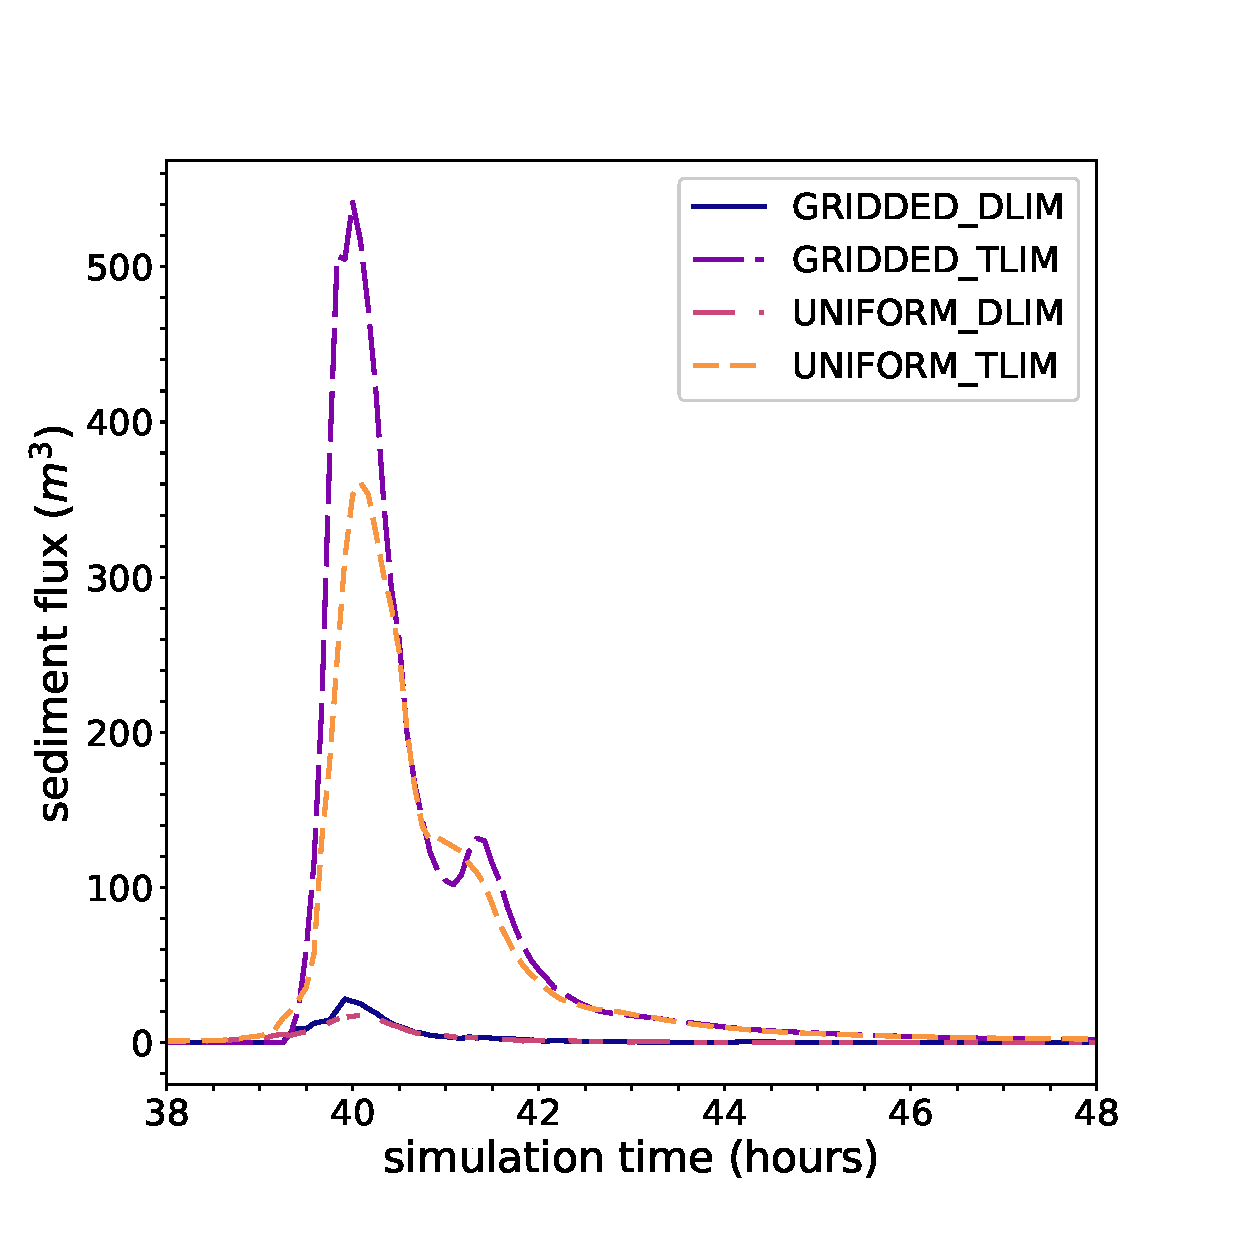
\includegraphics[width=14cm]{chp06_figures_scripts/figure_boscastle_sedigraph_ensemble.eps}
\caption{Boscastle sediment flux (total sediment volume output per hour at catchment outlet for each erosion-enabled simulation of the 2004 Boscastle event listed in Table \ref{table_ensemble_experiments}.}
\label{fig_boscastle_sedigraph_ensemble}
\end{figure}

\begin{figure}[t]
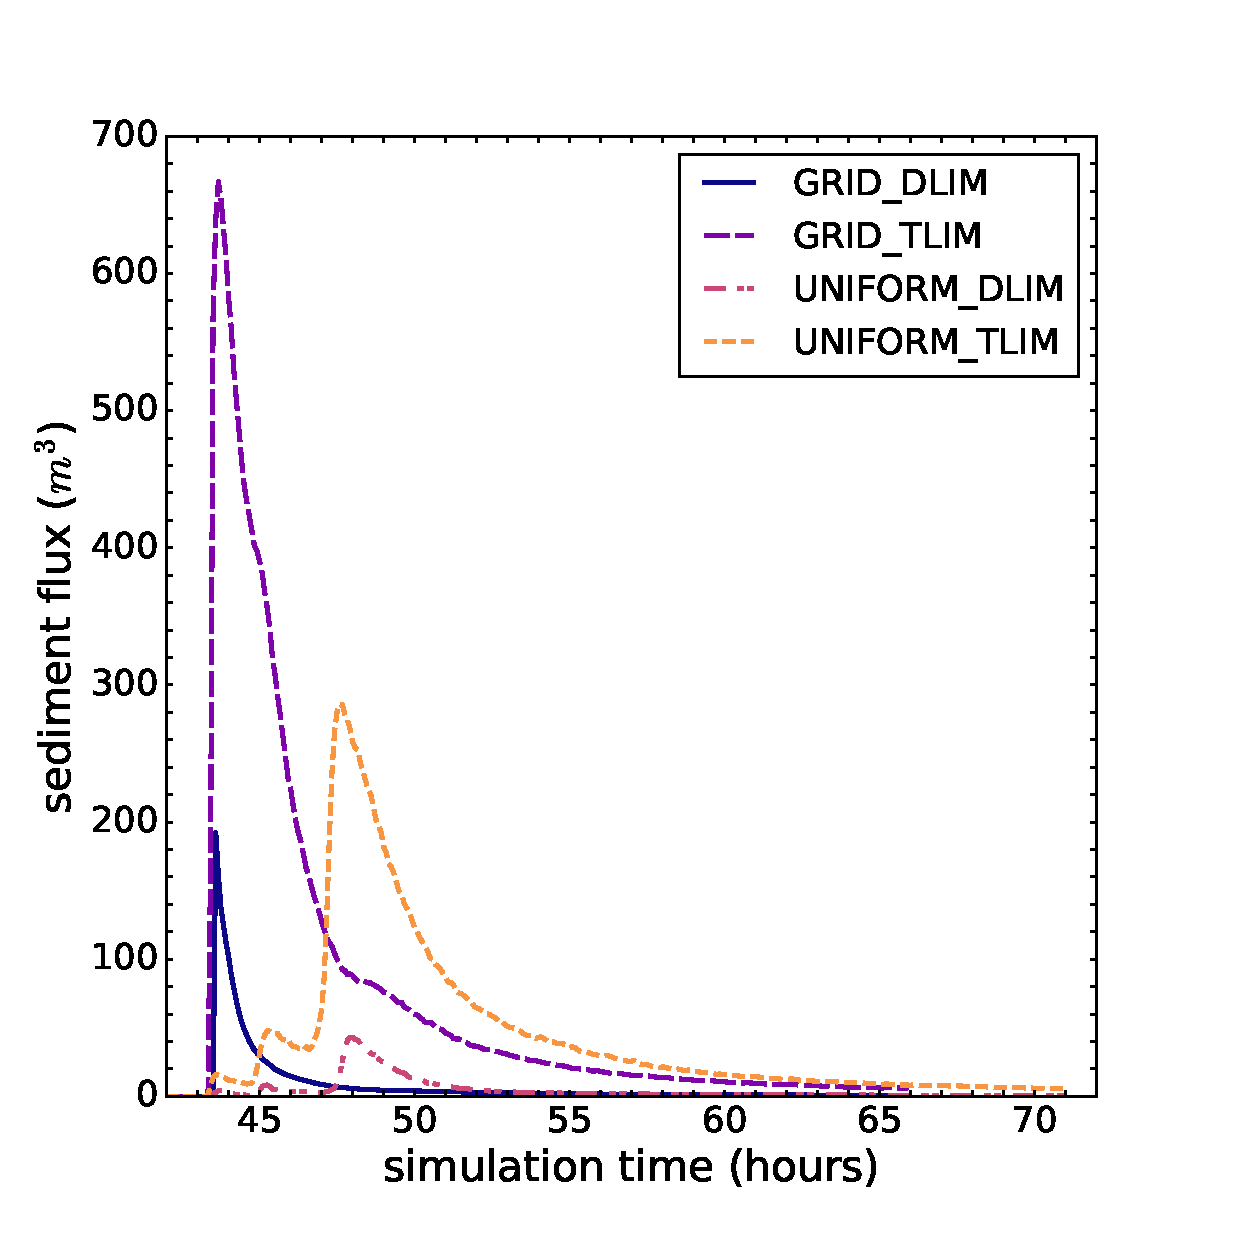
\includegraphics[width=14cm]{chp06_figures_scripts/figure_ryedale_sedigraph_ensemble.eps}
\caption{Ryedale sediment flux (Total sediment volume output per hour at catchment outlet) for each erosion-enabled simulation of the 2005 Ryedale event listed in Table \ref{table_ensemble_experiments}.}
\label{fig_ryedale_sedigraph_ensemble}
\end{figure}

% Describe planform variations in erosion and deposition
\subsection{Spatial variations in sediment and bedrock erosion}
The main spatial variation seen in sediment erosion is seen within river channels. The amount of erosion in each simulation was highly sensitive to parameterisation choice of the sediment erosion and transport law, with the choice of rainfall input data (gridded vs uniform) being only a secondary controlling factor on the spatial distribution of erosion, all other factors being equal. This behaviour was seen on all simulations, shown in Figures \ref{fig_boscastle_2dplan_erosion_ensemble} and \ref{fig_ryedale_2dplan_erosion_ensemble}. 

To highlight the variation in erosion along the river channel, longitudinal profiles showing the average change in elevation after the storm are shown in Figures \ref{fig_boscastle_swath_tlim} and \ref{fig_ryedale_swath_tlim}. The longitudinal profile shows the variation in erosion along the main channel within each catchment, averaged along a 10m wide swath centred on the midpoint of the channel. The swath profiling technique is adapted from \citep{hergarten2014extracting}. To reduce the number of points plotted along the swath profile, erosion is also averaged longitudinally, using bins spaced every 200m in the Ryedale catchment and every 50m in the Valency catchment.

% Swath profiles
% Boscastle TLIM
\begin{figure}[htb]
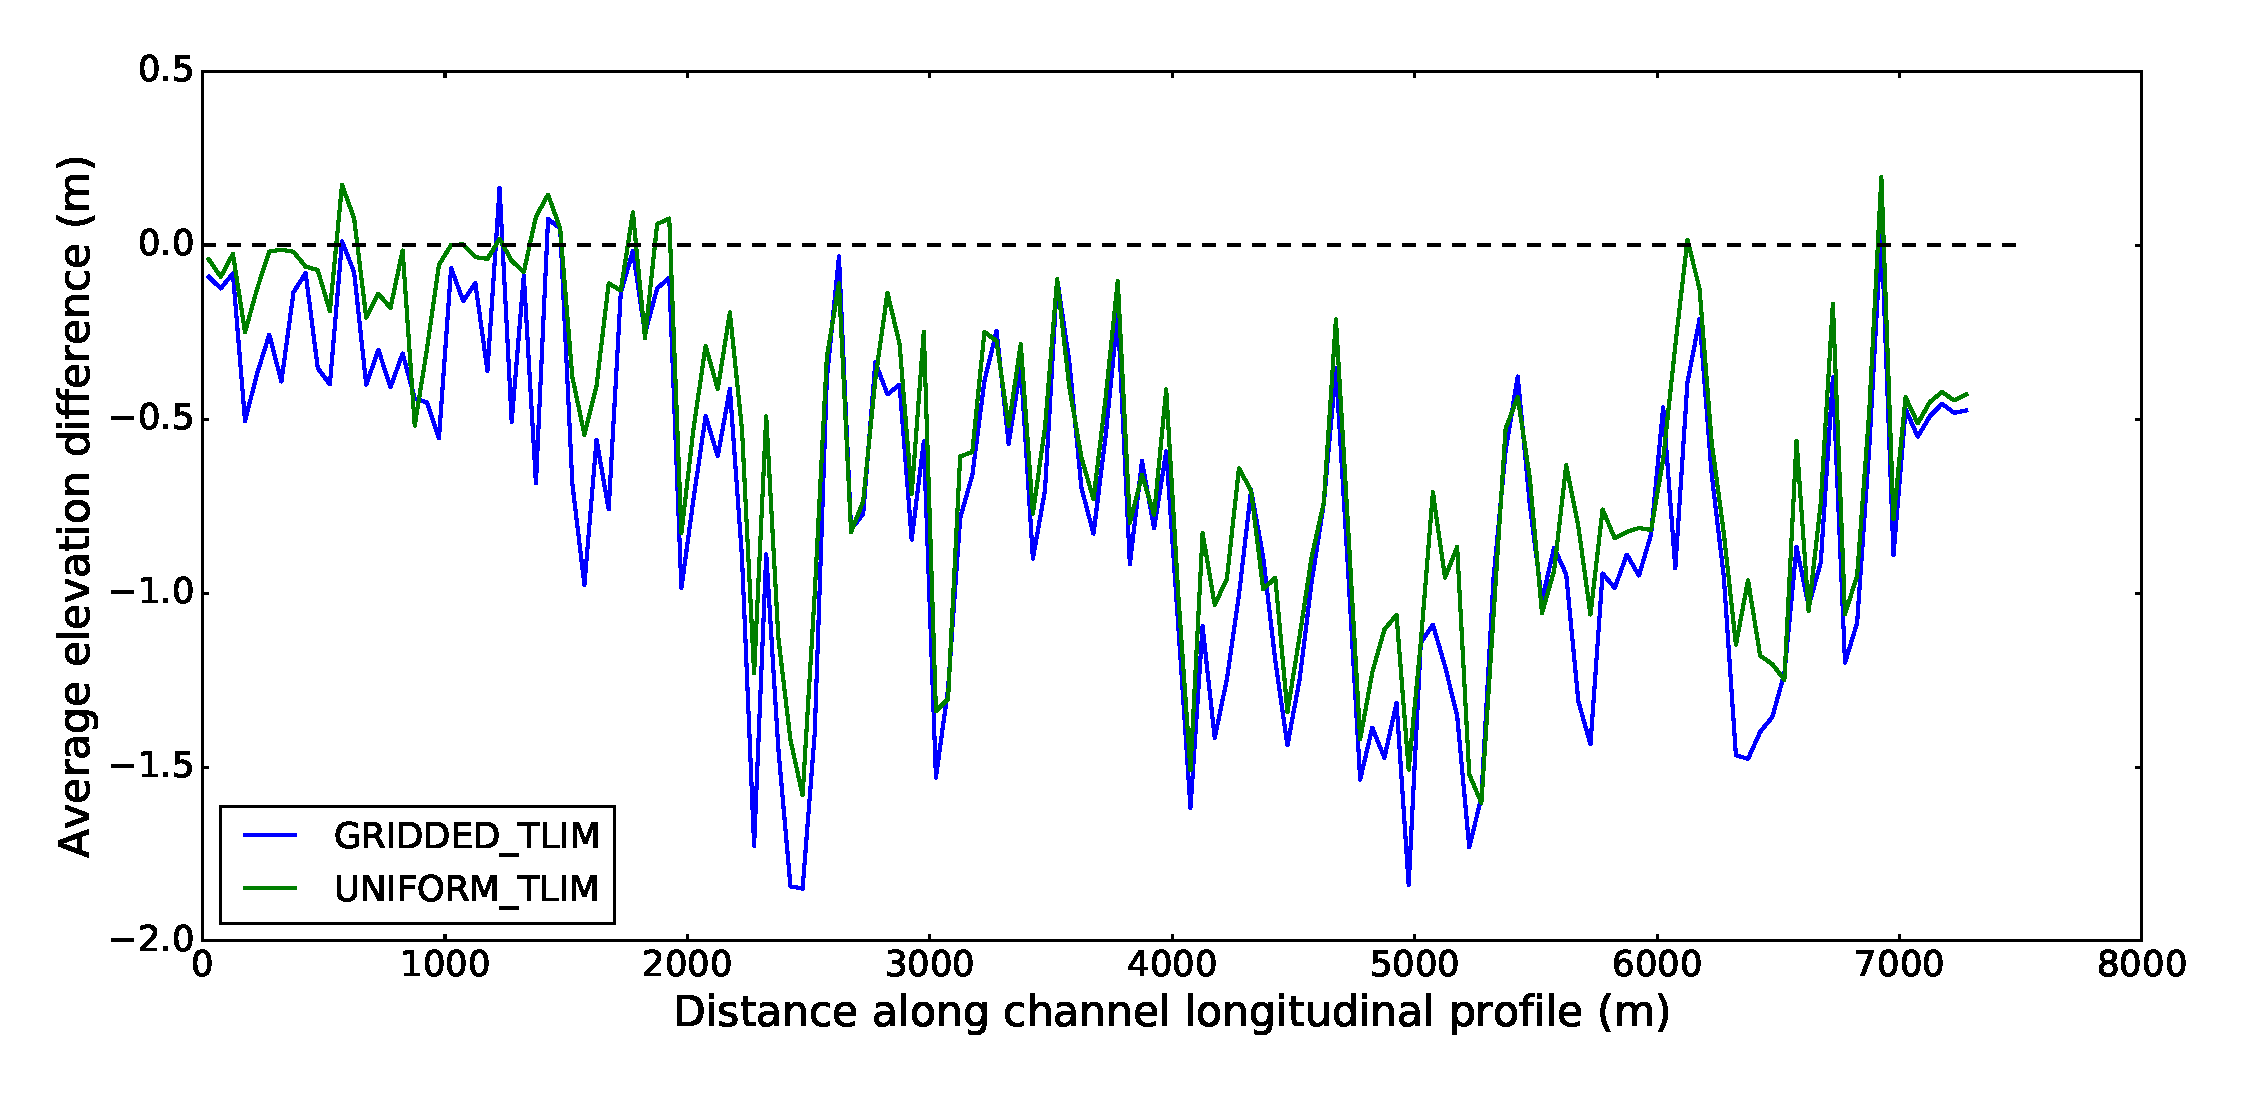
\includegraphics[width=14cm]{chp06_figures_scripts/fig_swath_profile_boscastle_erode_tlim.eps}
\caption{Channel averaged elevation difference along the main river channel in the Valency catchment. Simulation using the transport limited erosion parametrisation. Longitudinal profile is averaged over bins spaced every 50m. Transverse averaging (across the channel) is done over a 10m wide section centred on the channel midpoint. Results from the GRIDDED\_TLIM simulation shown in blue and the UNIFORM\_TLIM simulation shown in green.}
\label{fig_boscastle_swath_tlim}
\end{figure}

% Ryedale TLIM
\begin{figure}[htb]
\includegraphics[width=14cm]{chp06_figures_scripts/fig_swath_profile_ryedale_erode_tlim.eps}
\caption{Channel averaged elevation difference along the main river channel in the Valency catchment. Simulation using the transport limited erosion parametrisation. Longitudinal profile is averaged over bins spaced every 50m. Transverse averaging (across the channel) is done over a 10m wide section centred on the channel midpoint. Results from the GRIDDED\_TLIM simulation shown in blue and the UNIFORM\_TLIM simulation shown in green.}
\label{fig_ryedale_swath_tlim}
\end{figure}

Swath profiling of the Valency river channel (Boscastle) shows overall a net incision in the channel area, under transport-limited erosion parameterisation, with only small sections of the channel showing net sediment deposition (elevation increase) on average. Most incision is predicted to occur in the mid to upper reaches of the channel, with relatively little incision in the lowest reach of the catchment. The difference between gridded and uniform rainfall inputs shows a minimal difference along the main profile, though there is a slight tendency for the incision seen in the gridded rainfall input simulation to be higher in most places than the simulation using uniform input, with the difference in incision amounts of the order of tens of centimetres at most.

The swath profiling of the Rye river channel within the Ryedale catchment shows a large variation in incision and deposition rates within the catchment, though there is still an overall tendency for net incision. The magnitude of both incision and deposition is higher in the mid to upper reaches of the Rye river channel, similar to the pattern observed in the Valency river. The differences in average elevation changes are not as clearly distinguishable between the gridded and uniform rainfall input parameterisations, magnitudes of erosional and depositional peaks are slightly higher in the lower reaches of the river channel, but in the mid to upper reaches the differences are more varied. 
 
% OTHER SWATH PROFILES? DLIM, WIDER SWATH HALF WIDTH PERHAPS FOR RYEDALE?????
%
%

% Plan view erosion diff maps
\begin{sidewaysfigure}[t]
\includegraphics[width=25cm]{chp06_figures_scripts/figure_boscastle_erosion_diff_ensemble.png}
\caption{Boscastle. River Valency main channel in vicinity of Boscastle village. Net difference in elevation after 72 hours simulation, showing the gridded and uniform rainfall simulations, for each of the two erosion law end-members (transport-limited and detachment-limited). Elevation change smaller than \(\pm\) 0.2m in magnitude is not shown for clarity. Boscastle harbour is located in the upper left corner of each figure.}
\label{fig_boscastle_2dplan_erosion_ensemble}
\end{sidewaysfigure}

\begin{sidewaysfigure}[t]
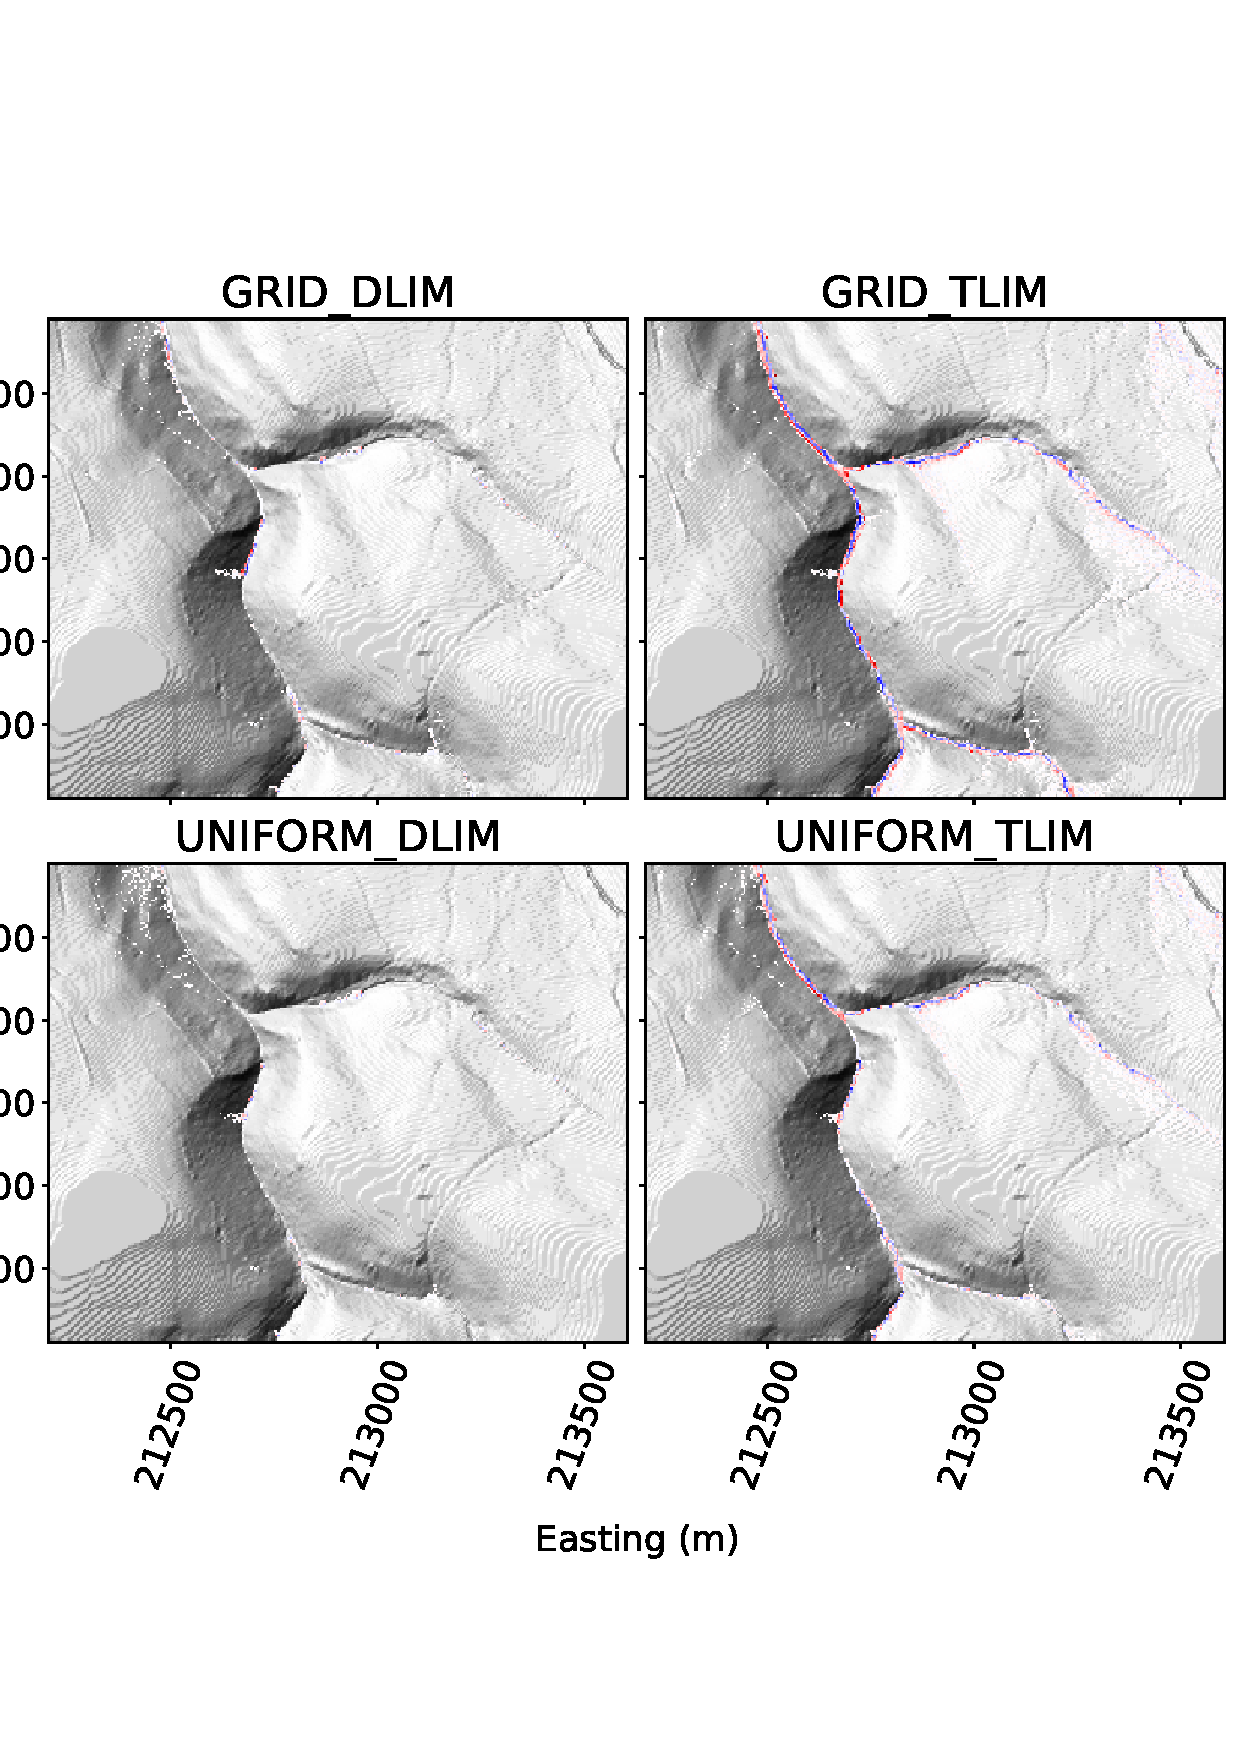
\includegraphics[width=18cm]{chp06_figures_scripts/figure_boscastle_erosion_diff_ensemble_SE.png}
\caption{Boscastle. South-east section of catchment showing the Lesnewth Stream tributary channel. Net difference in elevation after 72 hours simulation, showing the gridded and uniform rainfall simulations, for each of the two erosion law end-members (transport-limited and detachment-limited). Elevation change smaller than \(\pm\) 0.2m in magnitude is not shown for clarity. }
\label{fig_boscastle_2dplan_erosion_ensemble_SE}
\end{sidewaysfigure}

% Plan view erosion diff maps
\begin{sidewaysfigure}[t]
\includegraphics[width=25cm]{chp06_figures_scripts/figure_ryedale_erosion_diff_ensemble.png}
\caption{Ryedale. South-east section of Ryedale catchment showing the area around the village of Helmsley. Net difference in elevation after 72 hours simulation, showing the gridded and uniform rainfall simulations, for each of the two erosion law end-members (transport-limited and detachment-limited). Elevation change smaller than \(\pm\) 0.2m in magnitude is not shown for clarity. }
\label{fig_ryedale_2dplan_erosion_ensemble}
\end{sidewaysfigure}

% Full extent erosion maps
\begin{sidewaysfigure}[t]
\includegraphics[width=25cm]{chp06_figures_scripts/boscastle_erodediff_grid_tlim.png}
\caption{Boscastle. Map of extent of catchment change in elevation greater than 0.02m. Change in elevation shown after 72 hours of model simulation using gridded rainfall and the transport limited erosion law. Output from the gridded rainfall input, transport-limited erosion simulatio(GRID\_TLIM). Logarithmic scale for erosion.}
\label{fig_boscastle_erodediff_grid_tlim}
\end{sidewaysfigure}

\begin{sidewaysfigure}[t]
\includegraphics[width=25cm]{chp06_figures_scripts/boscastle_erodediff_uniform_tlim.png}
\caption{Boscastle. Map of extent of catchment change in elevation greater than 0.02m. Change in elevation shown after 72 hours of model simulation using uniform rainfall and the transport limited erosion law. Output from the uniform rainfall, transport-limited simulation (UNIFORM\_TLIM). Logarithmic scale for erosion.}
\label{fig_boscastle_erodediff_uniform_tlim}
\end{sidewaysfigure}

% RYEDALE lower reaches
\begin{figure}[htb]
\includegraphics[width=16cm]{chp06_figures_scripts/fig_ryedale_lower_erodediff_grid_tlim.png}
\caption{Ryedale. Map of extent of catchment change in elevation greater than 0.02m. Change in elevation shown after 72 hours of model simulation using gridded rainfall and the transport limited erosion law. Output from the gridded rainfall input, transport-limited erosion simulation (GRIDDED\_TLIM). Logarithmic scale for erosion.}
\label{fig_ryedale_erodediff_lower_grid_tlim}
\end{figure}

\begin{figure}[htb]
\includegraphics[width=16cm]{chp06_figures_scripts/fig_ryedale_lower_erodediff_uniform_tlim.png}
\caption{Ryedale. Map of extent of catchment change in elevation greater than 0.02m. Change in elevation shown after 72 hours of model simulation using uniform rainfall and the transport limited erosion law. Output from the uniform rainfall, transport-limited simulation (UNIFORM\_TLIM). Logarithmic scale for erosion.}
\label{fig_ryedale_erodediff_lower_uniform_tlim}
\end{figure}

\section{Discussion}

% Broader context of results
The relationship between the spatial distribution of rainfall and the erosional response of a river catchment has yet to be thoroughly explored. This analysis has sought to better understand how erosional processes are sensitive to the spatial detail of precipitation in the context of flash flood events from intense rainfall. Improving our understanding of the relationship between rainfall patterns and erosional processes will has two beneficiaries: 1) The short term environmental forecasting community will be able to better assess control that  rainfall distribution has on sediment dynamics and erosion patterns. In the absence of spatially variable input data for environmental prediction, modellers will at least be able to quantify the potential uncertainty involved in sediment flux predictions in the absence of such data. 2) Within the context of longer term landscape evolution, this study contributes to understanding the importance of individual storm events in driving landscape change over geological timescales. Current parameterisation of rainfall heterogeneity in long term landscape evolution modelling is simplistic at best, and this results of this study can be used to guide rainfall parameterisation in landscape evolution model development. 

% Critical analysis of major findings.
The findings in this study are based on simulating historic flash flood events using a cellular automaton  numerical model, the HAIL-CAESAR model (Chapter \ref{chapter_HAIL-CAESAR}). As such, the conclusions drawn from these experiments will be influenced by the individual characteristics of each catchment, though they were selected to be representative of typical upland catchments in the UK. It is expected that simulation of different catchments and events may produce somewhat different outcomes, but the overall findings should be applicable to other modelling situations. 

\subsection{Sensitivity to erosion law and rainfall heterogeneity} 
One key finding from the experiments, exhibited in both case studies, is that erosion law choice in the model is a more dominant control on sediment flux rather, rather than the spatial detail of precipitation. The erosion-enabled simulations in these experiments represented two end-members of sediment transport and erosion laws (As in Table \ref{table_ensemble_experiments}), transport-limited and detachment-limited. The transport-limited law simulations predict much greater sediment flux and erosion than their detachment-limited counterparts. In terms of sediment flux and erosion, the role of rainfall input data spatial resolution played only a secondary role in determining erosion amounts. The size of the catchment was less important in this respect, with even the smaller Boscastle catchment (18km\(^2\)) showing a marked sensitivity to the choice of erosion law. The sediment flux output from each catchment during the storm showed an order of magnitude difference between detachment and transport-limited erosion parameterisations, given the same rainfall spatial inputs. In contrast, the difference in sediment flux between uniform and gridded rainfall simulations was much smaller in both case study simulations.

Despite this study showing choice of erosion law being the dominant factor in controlling sediment flux, the study does confirm previous reports of increased sediment outputs from simulations using spatially heterogeneous rainfall data to drive simulations. \citet{coulthard2016sensitivity} reported that using finer resolution rainfall data at 5km grid spacing (also derived from meteorological radar) resulted in a doubling of sediment yields from a similar sized upland catchment (415km\(^2\)). The key difference in their findings was that the result was observed after a much longer simulation time of 30 years, using a 10-year rainfall record looped three times over the course of the simulation. While the rainfall data used in \citet{coulthard2016sensitivity} contain maximum rainfall intensities approaching those observed in the Boscastle and Ryedale storms used here, it is not clear whether they were part of prolonged storms over catchment, or were merely brief, localised cloudbursts. In other words, it cannot be determined whether the increase in sediment output observed in the \citet{coulthard2016sensitivity} gridded rainfall simulations is due to a particular storm in the 10 year rainfall record, due to cumulative erosive effects of lower intensity but higher frequency rainfall events, or some combination of both. The work presented in this chapter suggests that rainfall heterogeneity, while it may account for slightly higher sediment yields in individual storms, does not necessarily reproduce the `order of magnitude' differences observed over longer simulations such as in \citet{coulthard2016sensitivity} that may feature multiple storm events. However, this apparent discrepency across timescales may be due to the specific characteristics of these particular storms studied -- other types of storm, different spatial distributions of rainfall, may produce different results.

\subsection{Comparison with observed geomorphic change post-flood}

The resulting geomorphic change from the Boscastle 2004 flood, and to a lesser extent, the Ryedale flood of 2005 were extensively surveyed in the aftermath of the flood. Both sets of simulations lacked a suitably high-resolution DEM representing the state of the catchment before the flood took place, so a detailed before and after assessment of the accuracy of the model predictions are not possible. However, comparison with the reports on the erosion and deposition with each catchment allow us to make an assessment of whether the simulations were in broad agreement with the observations recorded after each flash flood event.

\subsubsection{Boscastle}
The geomorphological changes from the Boscastle flood were extensively mapped and recorded in an Environment Agency commissioned report carried out by \citet{wallingford2005flooding}. The reported amount of downcutting within the main Valency river channel was 1--2 metres in places. The transport-limited simulations predicted  a similar magnitude of downcutting in places, but also tended to overestimate the amount of downcutting, predicting up to 4m in places, which was not confirmed by the \citet{wallingford2005flooding} report. The detachment-limited simulations typically underestimated the amount of erosion and downcutting, particularly in the upper tributaries of the catchment, where little to no erosion was predicted, yet ground surveys post-flood reported substantial erosion within the channels. 

Substantial channel widening of up to 3--4m in places was reported in the HR Wallingford report. The HAIL-CAESAR model does not currently account for lateral channel erosion, and therefore there is no parameterisation of channel avulsion by lateral forces acting on the river bank in these simulations. The model allows a form of channel widening to take place through downcutting by water that has overtopped the channel banks, but this is not the primary mechanism through which channel widening occurs \citep{parker1976cause}. Future enhancements to the HAIL-CAESAR model would be needed to allow lateral channel widening to be investigated in the typical sense, similar to the implementations in \citet{murray1997properties,Coulthard2013}. The simulations presented in this chapter therefore do not reflect the channel widening reported in the post-flood geomorphological survey.

One area in which the gridded rainfall simulations performed better than the uniform rainfall inputs was in the tributaries in the south-east area of the catchment. The ground survey after the Boscastle flood noted significant amounts of erosion to in the tributaries on the south side of the river Valency. The tributary shown in Figure \ref{fig_boscastle_2dplan_erosion_ensemble_SE} was observed as having up to 1--2m of downcutting along its course. The gridded transport limited simulation more accurately predicted this than the corresponding uniform rainfall input simulations. It is notable that the regions of the catchment with the highest rainfall input -- mainly the southern and eastern fringes of the catchment -- fed into the tributaries that experienced the channel downcutting (see Figure \ref{fig_boscastle_rain_totals}). In this particular case it is evidence that high resolution of rainfall input data can better resolve the pattern of erosion on the ground.

Deposition of sediment was noted along most sections of the lower reaches of the Valency floodplain. The transport-limited simulations predicted sediment deposition in the small floodplain areas immediately adjacent to he river channel, but substantially overpredicted the amount of sediment deposition in places, predicting as much as 2--3m of deposition. Ground surveys, while noting deposition of sediment in many places, reported sediment deposition on the order of centimetres, not metres. The overestimation of deposition was present in both the gridded and uniform rainfall simulations, reinforcing the conclusion that uncertainty in the choice and paramterisation of sediment transport law is a stronger controlling factor than the spatial heterogeneity of rainfall.

Large sediment deposits were recorded after the event in the harbour area of Boscastle village \citep{wallingford2005flooding}. Notably, all simulations failed to predict this correctly, in fact predicting net sediment erosion in the harbour area (Figure \ref{fig_boscastle_2dplan_erosion_ensemble}, north-west corner). The discord between observations and model predictions in the harbour area may arise from the poor parameterisation of the interface where the catchment drains out into the sea in this area. The sea and tide in the harbour acting as a natural dampener to water flow velocities in reality, which would be expected to encourage deposition of sediments here.

\subsubsection{Ryedale}

Geomorphic change in the aftermath of the Ryedale was not as extensively surveyed compared to the Boscastle event. However, several studies noted general observations regarding the geomorphic impact of the event \citep{dong2006evaluation,wass2008investigation,hopkins2012knowledge}.
Channel downcutting was substantial, with 2--3m reported in the upper tributaries of the Rye catchment \citep{wass2008investigation,hopkins2012knowledge}. This pattern of channel incision was generally captured in the transport-limited simulations of the Ryedale flood but not in the detachment-limited simulations which tended to under-predict channel incision in the upper reaches of the catchment. Sediment deposition was reported in the lower reaches of the catchment, particularly in the village of Helmsley, but was not mapped extensively, unlike the Boscastle case. The simulations show areas of sediment deposition and erosion on the orders of 0.5--3m around the Helmsley area and the surrounding flood plain. Photographic evidence \citep{dong2006evaluation,hopkins2012knowledge} however, suggests these predictions are somewhat over-estimates of the ammount of incision and deposition in the floodplain area around Helmsley.

The Ryedale storm was noted for its triggering of over 100 shallow landslides within the catchment \citep{galiatsatos2007assessment,dong2006evaluation,
wass2008investigation}. The treatment of landsliding in the HAIL-CAESAR model is simplistic, based on a simple critical slope threshold required to trigger landslides, and as a result the reported landslides went largely unpredicted by all of the simulations. More complex models of landsliding are able to account for the role of soil saturation and pore water pressure in triggering of shallow landslides \citep[e.g.][]{iverson2000landslide,crosta2003distributed}. 

\subsection{Implications for longer-term landscape evolution}
The experiments presented in this chapter have focused on the hydrogeomorphic response to single severe storm events, events which produced floods with return periods of 1 in 330 years (Ryedale) and 1 in 1300 years (Boscastle). The amounts of river channel incision predicted as a result of these storms is comparable to that predicted by studies of landscape evolution on scales of 1000 years, for example a study of a similar upland river basin by \citep{coulthard2016sensitivity} predicted channel incision amounts of 0.5--5m over 1000 years. Ground surveys after both events \citep{wallingford2005flooding,dong2006evaluation} revealed somewhat lower channel incision amounts, though of the same order of magnitude (1--3m). The experiments presented here, using the same sediment transport law in the \citet{coulthard2016sensitivity} study, predict comparable amounts of channel incision during a single storm event. Previous studies of upland catchments in the UK that have experienced similar flash flood events have responded in a similar fashion \citep{johnson2002flooding,milan2012geomorphic}, showing catchment sediment fluxes far higher than typical for similar sized catchments \citep[e.g.][]{johnson2002annual}. If the flood return periods are assumed to be broadly correct, these simulations, along with previously published field studies, support the view that the majority of sediment erosion occurs during infrequent but high magnitude flood events, rather than through gradual processes or more frequent but lower magnitude events.

               
\subsection{Limitations}
The findings in this study are based on the outcomes of numerical simulations and data that are naturally simplifications of real landscapes and real rainfall events. Testing the potential for the HAIL-CAESAR model to forecast erosive episodes during flash flooding is limited due to the lack of pre- and post-event digital terrain models, therefore, only generalised comparisons can be made about the model's predictive ability and the ground surveys of geomrophic change carried out after the events. 

A number of assumptions were made about the catchment, due in part to the complexity and number of environmental processes parameterised in the numerical model. Sediment transport processes are driven by the overland flow of water, and are therefore sensitive to the choice of hydrological and hydraulic parameters. Hydrological parameters such as the TOPMODEL \(m\) parameter, or Manning's \(n\) are difficult to determine without extensive field calibration. In this study, reported values of from previous studies in similar catchments were used as guidance, and in the case of the TOPMODEL \(m\) parameter, sensitivity analysis was done (Chapter \ref{chapter_flood_model_sensitivity}) to determine the most appropriate value.   

Certain types of geomorphic change that were reported in post-event ground studies, such as channel avulsion in the Boscastle flood, and landsliding in the Ryedale event, are only simplistically represented in the numerical model. The full range of catchment erosional processes, such as lateral river bank erosion and mass movement cannot be fully explored in terms of sensitivity to rainfall spatial distribution. Nonetheless, the model captures the essential components of landscape evolution (overland flow and sediment transport by water) and their sensitivity to rainfall spatial distribution within a river catchment.


                       
\section{Conclusion}
The study was designed to test whether erosional processes in river catchments are sensitive to the spatial distribution of rainfall inputs, within the context of an individual severe storm.
These experiments have shown that it is the choice of erosional parameterisation in the model, and not necessarily the resolution of rainfall input data, that has a first-order control on the total sediment yields from a catchment and the magnitude of river channel incision during a simulated event.

Nevertheless, a further conclusion can also be made that rainfall spatial distribution does have an impact on sediment outputs and distribution of erosion in a catchment during an intense rainfall event, but in the cases shown here, it is a secondary control when compared to the choice and parameterisation of the erosion or sediment transport law. Where there is notable rainfall heterogeneity in a storm, spatially distributed rainfall data can be used to more accurately predict local variations in channel incision within the catchment, as was evident in the observed and predicted erosion patterns in the smaller Boscastle catchment.

The study has touched upon whether landscape evolution models may be used for shorter-term forecasting tools to predict the impact of flash floods on the landscape, should predicting areas of channel erosion and deposition. There are still a number of limitations in current landscape erosion models that prevent them being used as tools with detailed predictive power, notably the sensitivity from the choice of sediment transport laws as highlighted above. Using rainfall radar data as input to the model also introduces a further source of potential error (Chapter \ref{chapter_metdata}), which further compounds the uncertainty in the eventual prediction made by using a LEM in such a way to provide forecasts of landscape erosion in a single severe rainfall event. 

The importance of high magnitude, low frequency storm events in being agents of longer term landscape evolution is reinforced by this study. The amounts of channel incision predicted by the model (and confirmed in previously published post-event surveys), shows that a single storm can have as much erosive impact as decades of higher frequency, lower magnitude events. If one were to extrapolate the differences in predictions from uniform and gridded rainfall inputs based on this study, the effect of rainfall spatial detail could not be said be said to play a primary role on longer term landscape evolution. However, cumulatively the small differences observed between uniform and gridded rainfall inputs to the model may become more pronounced over longer-term landscape evolution simulations. It is important to acknowledge that these findings are based in the context of individual events, and other factors and feedbacks may come into play over longer timescales.











%\chapter{Sensitivity of landscape evolution to the details of precipitation patterns using NWP model data}

%\chapter{A spatially-limited storm generation model for long-term landscape evolution modelling}
%\chaptermark{Storm morphology controls on topography}
%
%\section{Intro}
%In landscapes where fluvial processes are the dominant mechanism of sediment erosion and transport, several models of fluvial incision have been proposed that parameterise hydro-meteorological conditions -- the transfer of water from the lower atmosphere to the land surface. Such models include the representation of rainfall input as discrete storm events, e.g. the Poisson pulse model of rainfall input (Tucker and Bras, 2000), models that incorporate the role of limited storm duration relative to runoff-time across the catchment (Solyom and Tucker, 2004), and the nature of orographic precipitation gradients the rainfall-runoff-erosion process (e.g. Anders and Roe, 2006; Han and Gasparini 2015). 
%
%
%\section{Hypothesis (mathematical model)}
%
%\textbf{In short}: Rate of fluvial incision is dependent storm size, depth, and position of storm cell relative to the catchment. This applies to large catchments or small storm cells, where the ratio of storm coverage to total catchment size is less than one. 
%
%\subsection{Catchment hydrology with limited storm cell sizes}
%For large catchments, or for small storm cells, the area of rainfall input, here termed the catchment wetted area, will be less than the total catchment drainage area. (See figure 1). This is denoted by the ratio: \(A_w/A\), where \(A_w\) is the wetted area. 
%
%%\begin{figure}
%%\label{stormcellbasin}
%%%\includegraphics[width=\textwidth]{drawing.png}
%%\caption{Two scenarios in the limited area storm model, both with storm cell areal coverage less than the total basin area. Storm wetted area \(A_{wa} \approx A_{wb}\). a) Storm cell centred far from catchment outlet point, ratio of wetted flow runoff length to max basin length, \(L_w/L\), is near 1. b) Storm cell centred close to outlet point, \(L_w\) is short relative to basin total length. The implications on peak discharge, and thus erosion rates, are discussed within the text.}
%%\end{figure}
%
%Given a catchment with a smaller contributing storm cell, there can be variability in the positioning of the storm relative to the catchment outlet point. This spatial variation in storm cell positioning will influence the storm hydrograph for each storm event. The total storm hydrograph time, \(T_h\) can be given by:
%
%\begin{equation}
%T_h = T_r + T_t
%\end{equation}
%
%Where \(T_r\) is the storm duration time, and \(T_t\) is the total runoff travel time from the most distant wetted point in the catchment to the outlet. The total runoff travel time is given by:
%
%\begin{equation}
%T_t = L_w/U_f
%\end{equation}
%
%where \( L_w \) is the longest wetted flow routing path in the catchment, \(U_f\) is the flow routing velocity, assumed to be approximately spatially constant. 
%
%\subsection{Deriving an approximation for discharge in storm-size limited catchments} 
%Solyom and Tucker (2004) note that similar derivations for peak discharge approximation are needed for environments where storm size is limited relative to catchment area, so I use their equations as a starting point. 
%
%Starting with the simple case of Hortonian (infiltration excess) overland flow, the discharge at a point in the river channel can be given by:
%
%\begin{equation}
%Q = (R - I)A_w
%\end{equation}
%where R is rainfall rate, I is infiltration rate, and \(A_w\) is the upstream wetted drainage area. The total volume of water in a given storm is stated as:
%
%\begin{equation}
%V = (R - I)A_w T_r
%\end{equation}
%
%where \(T_r\) is the storm duration time. As per Solyom and Tucker (2004) the total flood hydrograph volume can be written as:
%
%\begin{equation}
%V = \int_{0}^{T_h} Q(t) dt
%\end{equation}
%
%The hydrograph can be non-dimensionalised by scaling with peak flow, \(Q_p\), and time can be normalised by the total flood hydrograph duration, \(T_h\) (after Willgose, 1989):
%
%\begin{equation}
%Q'(t') = Q(t)/Q_p
%\end{equation}
%where
%\begin{equation}
%t' = t/T_h
%\end{equation}
%
%Then the non-dimensionalised flood-hydrograph volume can be written as such:
%
%\begin{equation}
%V = Q_p T_h \int_{0}^{1} Q'(t') dt'
%\end{equation}
%
%Assuming constant rainfall, \(R\), and infiltration rates, \(I\), peak discharge can be written as a function of runoff rate, storm duration, storm wetted area, and wetted flow route length:
%
%
%%\begin{equation}
%\begin{align}
%\label{peakdischarge}
%Q_p &= \frac{V}{T_h \int_{0}^{1} Q'(t') dt'} \
%    &= \frac{1}{T_h} \frac{(R-I) A_w T_r}{F_{hs}} \
%    &= \frac{(R-I)A_w}{F_{hs}} \frac{T_r}{T_r + L_w/U_f} 
%\end{align}
%%\end{equation}
%
%where \(F_{hs}\) is a hydrograph `shape-factor' equal to the integral in equation (8). \(F_{hs}\) goes to one for steady state run off conditions (i.e. a flat or rectangular hydrograph)
% 
%According to equation \ref{peakdischarge}, peak discharge will vary according to the catchment wetted area to wetted flow runoff length ratio, \(A_w/L_w\), and the ratio of storm duration, \(T_r\), to the total hydrograph duration. Also note that \(A_w\) and \(L_w\) are not independent of each other, and increasing \(A_w\) can increase \(L_w\). (This is not true in the Solyom and Tucker (2004) application of this equation as rainfall is assumed to spatially uniform over the total catchment area.)
%
%\subsection{Assumptions}
%
%\begin{itemize}
%\item Storm cell is stationary (does not track across the basin for the duration of the storm)
%\item Storm cell is a single cell. (i.e. not multiple cells scattered across the basin)
%\item Flow routing velocity is uniform. (Not entirely true assumption, routing time is slower on hillslopes, but the effect can be ignored if drainage density is relatively uniform (Solyom and Tucker (2004)).
%\item Rainfall rate and infiltration rate constant for duration of storm.
%\item Simple infiltration-excess (Hortonian) hydrological state.
%
%\end{itemize}
%It may be possible to modify the model to account for one or more of these assumptions.
%
%
%\subsection{Fluvial erosion}
%(Deriving a similar expression for fluvial incision in a detachment-limited environment here, incorporating the above non-steady discharge approximations for limited storm-area cases) 

%The rate of incision at any given point in a fluvial, bedrock channel is typically given as a function of excess shear stress, that is to say a certain threshold of shear stress exerted by the fluid flow of a river must be exceeded to detach bedrock material (Howard and Kerby, xxxx):

%\begin{equation}
%\epsilon = K_e(\tau - {\tau}_c)^\gamma
%\end{equation}
%
%where shear stress, \({\tau}_c \) and critical shear stress, \( {\tau}_c \), are given by a function of the local discharge \(q\), channel gradient, \(S\) and a shear stress coefficient, \(K_t\).
%
%Traditional models of fluvial incision typically consider discharge at any given point on the landscape as a function of local channel gradient and upstream constributing drainage area, such as the simple stream power law equation for fluvial incision in bedrock channels;
%
%\begin{equation}
%E = 
%\end{equation}


%\chapter{Co-evolution of rainfall patterns and landscapes}
%
%\textit{It would be nice to look at this if there was time (there probably won't be though!) I had a rough framework sketched out and partially implemented for how this would be done using CHILD and WRF together. Maybe one for the future instead.
%}

\chapter{Conclusions}
\label{chapter_conclusion}
\chaptermark{Conclusions}

\section{Review of aims and overview of results}

I set out to investigate the sensitivity of hydrogeomorphic processes to rainfall spatial variability during intense rainfall events. The aims of the thesis presented in Chapter \ref{chapter_intro} consisted of two scientific aims and one technological aim to support them. The scientific aims were to investigate the influence of using spatially variable rainfall input data on a) flood inundation predictions and b) sediment flux and distribution of erosion and deposition; both aims addressed within the context of flash flooding events from intense rainfall. To address these questions, a hydrodynamic landscape evolution model was developed based on an existing model, capable of carrying out ensemble-style simulations on high-performance computing (HPC) services (Chapter \ref{chapter_HAIL-CAESAR}. To build on previous studies that have investigated the role of rainfall spatial resolution in isolation, or with other competing factors, a secondary variable was introduced: the choice of erosional process parameterisation in the model. This study is believed to be the first to investigate the sensitivity of rainfall resolution and erosional process parameterisation in tandem, and to assess which has the greater control on hydrogeomorphic processes in river catchments. It is also one of few studies to investigate the role of these two competing factors within the context of an individual flash flooding event from intense rainfall. 

The two core scientific hypotheses (presented in detail in Chapter \ref{chapter_events}, Section \ref{section_experiment_design}) stated:

\begin{enumerate}
\item Flood inundation modelling is sensitive to the spatial detail of precipitation inputs.
\item Erosional processes in river catchments are sensitive to the spatial distribution of rainfall inputs.
\end{enumerate}

These results from the testing of these hypotheses are discussed in the conclusions made in Chapters \ref{chapter_flood_model_sensitivity} and \ref{chapter_hydrogeomorph} and are summarised in the following sections:

\subsection{Flood-inundation model sensitivity}
Flood inundation model predictions are sensitive to spatial distribution of rainfall inputs, specifically the use of 1km gridded rainfall data, when compared to using uniform avaeraged data as model input. Predicted hydrological discharge is higher using gridded rainfall inputs, though not necessarily more accurate when compared to measured discharges during the respective flood events simulated. In the Boscastle case study, river discharges more closely matched the observed data, whereas in the Ryedale event, uniform rainfall inputs into the model actually produced a better match to observed data. The choice of erosional process parameterisation plays only a secondary role in hydrological response. 

\subsection{Erosion and sediment flux sensitivity}
Fluvial erosional processes in river catchments are somewhat sensitive to the use of spatially variable rainfall input data to the model, though it is only of secondary importance when compared to the sensitivity observed in the use of different erosional process law parametrisations. The difference in sediment outputs were much greater under a transport-limited type erosion law, compared to a detachment-limited one. The effects from using spatially variable rainfall input data on sediment fluxes were less noticeable in comparison, but still had a measurable effect on sediment fluxes. Using spatially variable rainfall data increased sediment yields in both case studies and under both types of erosional parameterisation.

\section{Key themes and synthesis}

It was set out to determine whether hydrogeomorphic processes in river catchments were sensitive to the spatial detail of rainfall input data. Numerical simulations using a hydrodynamic landscape evolution model have indicated that resolving the spatial detail in rainfall structure during severe storms has a demonstrable effect on both hydrological and sediment fluxes. (e.g. Figures \ref{fig_boscastle_hydrograph_ensemble}, \ref{fig_boscastle_sedigraph_ensemble}, \ref{fig_ryedale_hydrograph_ensemble}, \ref{fig_ryedale_sedigraph_ensemble}). Though the magnitude of the sensitivity varied between experiments, there was a general increase in peak discharge and peak sediment flux in simulations with gridded rainfall data used as the rainfall input, compared to simulations that used a single, spatially uniform value for rainfall. Existing studies investigating landscape evolution model sensitivity to rainfall resolution \citep{coulthard2016sensitivity} have noted similar increases in water discharge and sediment yields when using spatially heterogeneous rainfall data. The results from the experiments presented in this chapter are broadly in agreement with the general findings of \citet{coulthard2016sensitivity} although the timescales simulated in this study are on the order of hours, rather than decades. The results presented here suggest that the effect of rainfall resolution sensitivity applies to hydrogeomorphic processes at the single storm event timescale, as well as landscape evolution over periods of decades to hundreds of years.

Opting to use spatially variable rainfall data at 1 km resolution was sufficient to observe sediment flux sensitivity to rainfall variability in a catchment as small as 12 km\(^2\). However, rainfall features equal to or greater in size than the catchment over which they rain upon may well be homogeneous enough in spatial extent and rainfall rate that a `uniform' approximation of their intensity is sufficient to represent the rainfall rate at all points in the catchment. From a hydrological perspective, as seen in the Boscastle catchment simulations, using a spatially variable rainfall input data source did not notably alter the outcome of the hydrological predictions (Figures \ref{fig_boscastle_2dplan_flood_ensemble_town}, \ref{fig_ryedale_2dplan_flood_ensemble_town}). However, in the Ryedale catchment simulations, the hydrological predictions were notably different based on the choice of rainfall input data resolution, affecting both the timing and magnitude of the resulting flood peak. It is possible that hydrological processes are less sensitive to rainfall spatial variability in smaller catchments than erosional processes are, although further systematic study would be necessary to determine exactly what the threshold catchment size might be where rainfall spatial variability becomes an issue in hydrological models.
%
%Talk about size of convective cell features. What is typical storm cell size and heterogeneity (decay from centre?).

\section{Technical advances}
The numerical simulation work in this project has been made possible by the development of a numerical landscape evolution model suitable for deployment on HPC services (Chapter \ref{chapter_HAIL-CAESAR}). The porting and development of landscape erosion and evolution models for HPC has thus far been under-exploited in the geomorphological modelling community. The development and parallelisation of the HAIL-CAESAR model as part of this thesis is an advancement of existing methods in computational modelling for hydro-geomorphology:

Firstly, the model's basis as a redevelopment of an existing model (CAESAR-Lisflood) provides a continuity and familiarity with the existing user base. Core functionality is preserved, which will hopefully encourage an uptake in use of the model amongst existing users of the CAESAR-Lisflood model. The translation of the original model's code, preserving the algorithms as closely as possible in a different programming language, ensures there is comparability between the original and redeveloped version of the model presented here. 

Secondly, in addition to the speed-up in simulation runtimes achieved, the ability to now use HPC facilities to conduct hydrogeomorphological modelling studies allows large-scale sensitivity analyses to be done, with multiple member `ensemble-style' simulations, in a similar fashion to numerical weather prediction model ensembles \citep{sivillo1997ensemble,klein2015variability}. In this study, six-member simulations per case study are are used for the main set of experiments (Table \ref{table_ensemble_experiments}), with ten member simulations used for the parameter sensitivity analysis in Chapter \ref{chapter_flood_model_sensitivity} (Table \ref{table-m-sens}). With sufficient computing resources, much larger ensemble simulations would be possible using the HAIL-CAESAR model.

\section{Future research and applications}
This study has touched upon the potential for using large ensemble-style simulations to assess sensitivity in landscape evolution modelling studies. Since numerical landscape evolution models typically contain a large number of parameters, particularly as they often combine multiple-process sub-models such as erosion, hydrology, hillslope processes, and other surface processes, a thorough exploration of parameter space is usually beyond the scope of many studies. Current applications of landscape erosion and evolution models rarely make use of multiple-member ensemble simulations, whereas this practice is more commonly found in hydrological modelling \citep{cloke2009ensemble,wong2015sensitivity} and numerical weather prediction \citep{sivillo1997ensemble}. Hydrogeomorphic and landscape evolution modelling studies have been late adopters of ensemble simulations, but this thesis as well as other projects \citep[e.g.][]{schaake2007hepex,skinner2017lemsi} highlight the timely applicability of ensemble-style simulations for future hydrogeomorphic research. The HAIL-CAESAR model could be used in this way in future studies to more rigorously assess model sensitivity to user-defined parameters in landscape evolution modelling. Taking advantage of the increase in computing power in recent decades with the HAIL-CAESAR model presented in this thesis would enable a rigorous exploration of model sensitivity to parameter-space, initial model conditions, input data quality, model resolution, and many other sources of potential uncertainty \citep{pelletier2015forecasting}.

Further development of the model would allow it to tackle large catchments at regional to continental scale, or very high resolution studies of smaller river catchments. High resolution topographic data already exists at resolutions of 0.2 to 0.5 m, primarily sourced from LiDAR-dervied topographic data. At this resolution, river channel and other geomorphological features can be resolved in great detail within the model domain. Although the data is readily available now, few modelling studies have yet made use of such high resolution data, partly because of limitations in computational resources and appropriately designed software. Notwithstanding, the HAIL-CAESAR model would require further development to address the scaling issues highlighted in Chapter \ref{chapter_HAIL-CAESAR}, in order to tackle model domains containing tens of millions of grid cells.

Predicting catchment response to intense rainfall events is a pressing societal issue. Current flood forecasting applications tend to focus primarily on the hydrological response of catchments without taking into account geomorphological change during such events. Future development of models in the flood-forecasting community could expand them to be more holistic simulators of catchment processes, including sediment erosion and transport, in addition to their core functionally of predicting flood inundation extents. 

\section{Future development of HAIL-CAESAR}

A number of interested parties have expressed interest in using HAIL-CAESAR for further landscape evolution and hydrological modelling. Future development work is outlined here.

\subsection*{Reach mode}
Development of the model in future would include the development of a `reach-mode' in addition to the `whole-catchment' mode currently implemented in the model. Reach-mode would be a configuration of the model that allows it to simulate localised sections of a river channel and surrounding area. Reach-mode is also feature of the progenitor to the HAIL-CAESAR model, CAESAR-Lisflood, and has applications where detailed simulations are required of particular sections of river channel, but not of the entire catchment. Reach mode (as part of CAESAR-Lisflood) has been employed in a number of studies to date (CITE) and would be a useful addition to the CAESAR modelling community. 

\subsection*{Process representation}
A number of processes in the CAESAR and CAESAR-Lisflood models were omitted in the HAIL-CAESAR development process because of time constraints and applicability to the research questions posed in this thesis. Additional process representation in the HAIL-CAESAR model could be facilitated by the implementation of the following additional subroutines in the model code:

\begin{itemize}
\item \textbf{Lateral channel erosion}. Currently only downcutting erosion and deposition is represented in the model. The lack of lateral erosion mechanisms was highlighted as a possible limitation in the HAIL-CAESAR model's ability to fully predict the amount and distribution in the Boscastle event documented in Chapter \ref{chapter_hydrogeomorph}

\item \textbf{Slope processes}. Slope processes in HAIL-CAESAR as well as CAESAR-Lisflood have very simple representations based on simple threshold gradients to initiate redistribution of slope material between adjacent cells. A number of more physically realistic slope process models exist that could be incorporated into the HAIL-CAESAR model.

\item \textbf{Groundwater}. Interest has been expressed by the developers of the British Geological Survey's CLiDE model in using HAIL-CAESAR as a basis for the development of a coupled groundwater--catchment hydrology and erosion model for use on HPC services. The groundwater components would be based on the algorithms in the existing CLiDE model, another CAESAR-based model with applications in environmental modelling and prediction \citep[e.g.][]{Barkwith2015}.

\item \textbf{MPI parallelisation}. HAIL-CAESAR was parallelised in a way to facilitate the use of multi-member ensemble simulations on shared-memory compute nodes. This method of parallelisation lends itself well to sensitivity analyses as demonstrated in this thesis, and moderately large domains and high-resolution data. However, to fully exploit the highest resolution datasets available, or to conduct regional to continental scale modelling studies, a different parallelisation strategy would have to be employed using what is termed `distributed-memory' parallelism, whereby the model domain is decomposed across multiple computing nodes. The most common approach to this is to use a parallelisation standard known as MPI -- the Message Passing Interface. Initial plans for the implementation of HAIL-CAESAR with the MPI software libraries are currently under development. Such work would require a considerable development effort but there are precedents for purely hydrological models being parallelised in this way before \citep{vivoni2011real}, and many of the techniques could be applied to landscape evolution models such as HAIL-CAESAR.

There has also been an interest expressed in using part of the HAIL-CAESAR model as an educational tool for teaching MPI parallesation, in part due to the cellular automaton modelling framework being a relatively straightforward modelling technique to parallelise over a 2D domain (Edinburgh Parallel Computing Centre -- personal communication).

\end{itemize}



\section{Summary}
This thesis has presented a novel method for simulating hydrological and geomorphological processes at the catchment scale using high-performance computing systems. This method was then applied to investigating the sensitivity of hydrogeomorphic processes to the spatial resolution of rainfall input data and erosional process parameterisation. It was found that while spatial variability in rainfall input data to models can affect the hydrological outputs of numerical models, predictions are not necessarily more accurate in all cases when using spatially variable rainfall input data. In terms of predicting sediment fluxes and erosion distribution, the choice of erosion law had a more pronounced effect on sediment fluxes compared to spatially variable rainfall input data. Notwithstanding, the use of spatially variable rainfall data in hydrodynamic landscape evolution models can in some cases better predict localised distribution of erosion within a river catchment. The findings and methodological developments pose a useful contribution to the future of hydrogeomorphological modelling and its applications in environmental prediction and forecasting.



% If using biblatex package

\printbibliography

% If using natbib package
%\bibliographystyle{apalike}
%\bibliography{literature}

% Comment the following THREE lines if you do NOT have an Appendix
\appendix
%\chapter{Linking high-resolution NWP model output with a landscape evolution model}
\label{appendix_wrf_lem}
\section{Introduction}

An introduction to the need for better forecasting of flash fooding events. Societal impacts etc. References to recent events in the UK. Rapid geomorphological change can accompany such events, leading to unexpected hydrological outcomes as most models assume static terrain surface during flood-inundation prediction.

Weather forecast models allow high resolution simulations to forecast spatial details of precipitations. Potential forecasting capability when coupled to hydrodynamic landscape evolution model. Relate to summer convective events which tend to be much more spatially focused (mesoscale) and can hence rainfall inputs can vary significantly across a catchment. NWP offers greater lead times than radar `nowcasting'. 

Can cite Pitt review (2008).

Need to investigate better linking of environmental models. E.g. NWP to Land Surface Flooding and Erosion models.

This chapter presents a framework for driving a landscape evolution model with output from NWP simulations. The framework is based upon further enhancements made to the HAIL-CAESAR model, described initially in Chapter \ref{chapter_HAIL-CAESAR}. The enhancements are described in the following section and then tested by the application of the model framework to test cases from intense rainfall events in the UK, previously investigate in Chapter \ref{chapter_hydrogeomorph}.

The work investigates whether a one-way coupled model can provide better forecasting ability over a model driven with coarser resolution rainfall radar data.

\section{Modelling framework}


\section{Method}

Two WRF simulations.

\begin{itemize}
\item Boscastle (2004)
\item Ryedale (2005)
\item Both events triggered flash floods, and the flooding was exarcebated by the mobilisation of sediment during the flood, leading to blocked river channels/channels with reduced capacity.
\end{itemize}

Model set up:
\begin{itemize}
\item Four domains, with the innermost domain centred on the river catchment of interest with a horizontal grid spacing of 200m. Outer domains have reolutions of 25km, 5km, and 1km.
\item Initialised with ECMWF data. (ERA-20C).
\end{itemize}

\textbf{Figure: WRF domain set up}

\textbf{Table: WRF parameters for each simulation}

\subsection{Modifications to the CAESAR-Lisflood model}
Description of model modifications to enable ingestion of high resolution rainfall data. I.e. describe the new rainfall runoff generation model. How it differs from the standard sem-distributed model (TOPMODEL) found in CAESAR-Lisflood.

A f\textbf{figure} would probably be useful here to aid the description of the model component. 

\subsection{Landscape evolution model set up}

No need to repeat the general model description in Chapter 5, just refer back. List the parameters for each simulation in a table though.

\subsection{Modelling framework}

\textbf{Figure: flowchart showing the set up of the two models and their integration}. Brief description here.

\section{Results}

\subsection{NWP modelling results}

\textbf{Show a figure of the rainfall outputs over the inner domain and overlain over the river catchment(2 figures, one for each case)}

\subsection{Landscape evolution/hydrology modelling results.}

Similar figures as to previous chapter of flood inundation and erosion spatial distribution. 

\section{Discussion} 

Discus differences with the rainfall radar chapter previously. Does 200m NWP simulations produce any noticable differences with the 1km gridded radar inputs and the uniform rainfall inputs. 


\chapter{Software availability}
\label{appendix_software}

\section{Radar data processing code}
The software for the radar data extraction and re-gridding for use in the HAIL-CAESAR/CAESAR-Lisflood models is available at the online software repository GitHub at: \url{https://github.com/dvalters/nimrod-toolbox/releases/tag/0.2}

\section{HAIL-CAESAR landscape evolution model code}
The HAIL-CAESAR landscape evolution modelling software is available at the online software repository GitHub at: \url{https://github.com/dvalters/HAIL-CAESAR/releases/tag/v0.9}

\section{Figure plotting software}
The code used to plot figures from the model simulation output in this thesis was part of the \textit{LSDMappingTools} package and can be found here: \url{https://github.com/LSDtopotools/LSDMappingTools}. The author contributed to a significant part of the LSDMappingTools software development during the course of the PhD.

%\chapter{Core code for the HAIL-CAESAR model}
%
%%\lstdefinestyle{customcpp}{
%%  belowcaptionskip=1\baselineskip,
%%  breaklines=true,
%%  %xleftmargin=\parindent,
%%  language=C++,
%%  showstringspaces=false,
%%  basicstyle=\footnotesize\ttfamily,
%%  keywordstyle=\bfseries\color{green!40!black},
%%  commentstyle=\itshape\color{purple!40!black},
%%  identifierstyle=\color{blue},
%%  stringstyle=\color{orange},
%% }
%%  
%%\lstinputlisting[language=C++,style=customcpp]{/mnt/SCRATCH/Dev/HAIL-CAESAR/LSDCatchmentModel.cpp}
%
%\chapter{NIMROD-processing code}
%\label{appendix_nimrod_code}
%
%\lstdefinestyle{mypy}{
%  language=Python,
%  backgroundcolor=\color{white}, %%%%%%%
%  basicstyle=\footnotesize\ttfamily,
%  breaklines=true,
%  otherkeywords={self},            
%  keywordstyle=\bfseries\color{blue},
%  emph={MyClass,__init__},          
%  emphstyle=\bfseries\color{purple!40!black},    
%  stringstyle=\color{green!40!black},
%  commentstyle=\color{red},  %%%%%%%%
%  frame=tb,                         
%  showstringspaces=false            
%}
%
%\section{NIMROD data conversion code}
%\lstinputlisting[language=Python,style=mypy]{/mnt/SCRATCH/Dev/nimrod-toolbox/NIMROD_convert.py}
%
%\section{NIMROD rainfall timeseries creation code}
%\lstinputlisting[language=Python,style=mypy]{/mnt/SCRATCH/Dev/nimrod-toolbox/NIMROD_timeseries.py}
%
%\section{Code for creating HAIL-CAESAR hydroindex file}
%\lstinputlisting[language=Python,style=mypy]{/mnt/SCRATCH/Dev/nimrod-toolbox/create_hydroindex.py}
%
%
%\chapter{Swath profiling algorithm and code}
%
%%\chapter{Configuration of the WRF model for the simulation of the North York Moors storm}
%
%%\chapter{Modifications made to the Weather Research and Forecasting model (WRF)}
%
%%\chapter{A one-way coupling framework for the WRF-CHILD model}
%
%\chapter{HPC computing simulations: set-up and compilation}
%
\chapter{Paper reprint}
\label{appendix_paper}

\textbf{Modelling Geomorphic Systems: Landscape Evolution}

\noindent
The content of Chapter \ref{chapter_landscape_evol} was adapted for an article in the British Society for Geomorphology's \textit{Geomorphological Techniques} article series. A reprint is included in this appendix.


\includepdf[pages={-}, pagecommand={}, scale=.9]{Landscape_Evolution_Modelling_Valters.pdf}


%APPENDICES
%
% 1. Code for the hail-caesar model (extracts)
% 2. Code for the NIMROD-processing script
% 3. Code for the long channel swath profiler (flowchart)


% If you need more than one appendix, then just use another \chapter command
%\chapter{Yet Another Appendix}

\end{document}
